\chapter{Learning Network Representations}
\label{sec:ch6}

Network-valued data differs from more traditional representations of data. Networks have a particularly useful topological structure: the manner in which the edges and nodes manifest gives useful information about relationships between the nodes. However, this structure comes with a drawback: the vast majority of machine learning, to date, is designed for tabular structures living in a space of features, where each data point is defined by a vector of scalar feature values. In this way of viewing data, each observation tends to be treated roughly independently (although possible relationships like correlations can still be found under the hood).

Even modern neural networks operate using this type of data. The entire field of \textit{representation learning}, a subfield of deep learning, uses dimensionality reduction techniques to bring data -- often images or text -- into a tabular space of features. Almost all well-known neural network architectures turn data into feature representations under the hood.

In fact, pretty much every other branch of machine learning and data science project data into some space where each datapoint can be viewed as a literal point in space, in which the axes correspond to properties (the features) of that datapoint. Representing data in this way is powerful and so it would be useful for us to be able to fluidly move between graph-space and feature-representation space.

In network-valued data, with $n$ nodes, there are $n!$ possible dependencies that could exist in the data (that is, each node could be dependent on the other nodes, which in turn are dependent on other nodes, so on and so forth, for all of the nodes in the network). To make this a bit more tractable to learn from, in network learning, we tend to serialize the network using one of the types of models which we learned about in Section \ref{sec:ch4:net-rep}. For network learning, the most common approach that we will use is the bag of edges approach in Section \ref{sec:ch4:net-rep:bagofnodes} approach. The idea is to turn each node into a data point living in feature-representation space.

There are a variety of ways we can do this, the most common of which tend to be the various types of spectral embeddings. When we have multiple networks, we will use a combination of the bag of nodes approach in Section \ref{sec:ch4:net-rep:bagofnodes} and the bag of networks approach in Section \ref{sec:ch4:net-rep:bagofnets}. In Figure \ref{fig:ch6:netrep}, one step is "choosing a suitable representation": that is what this chapter is all about.

\begin{figure}[h]
    \centering
    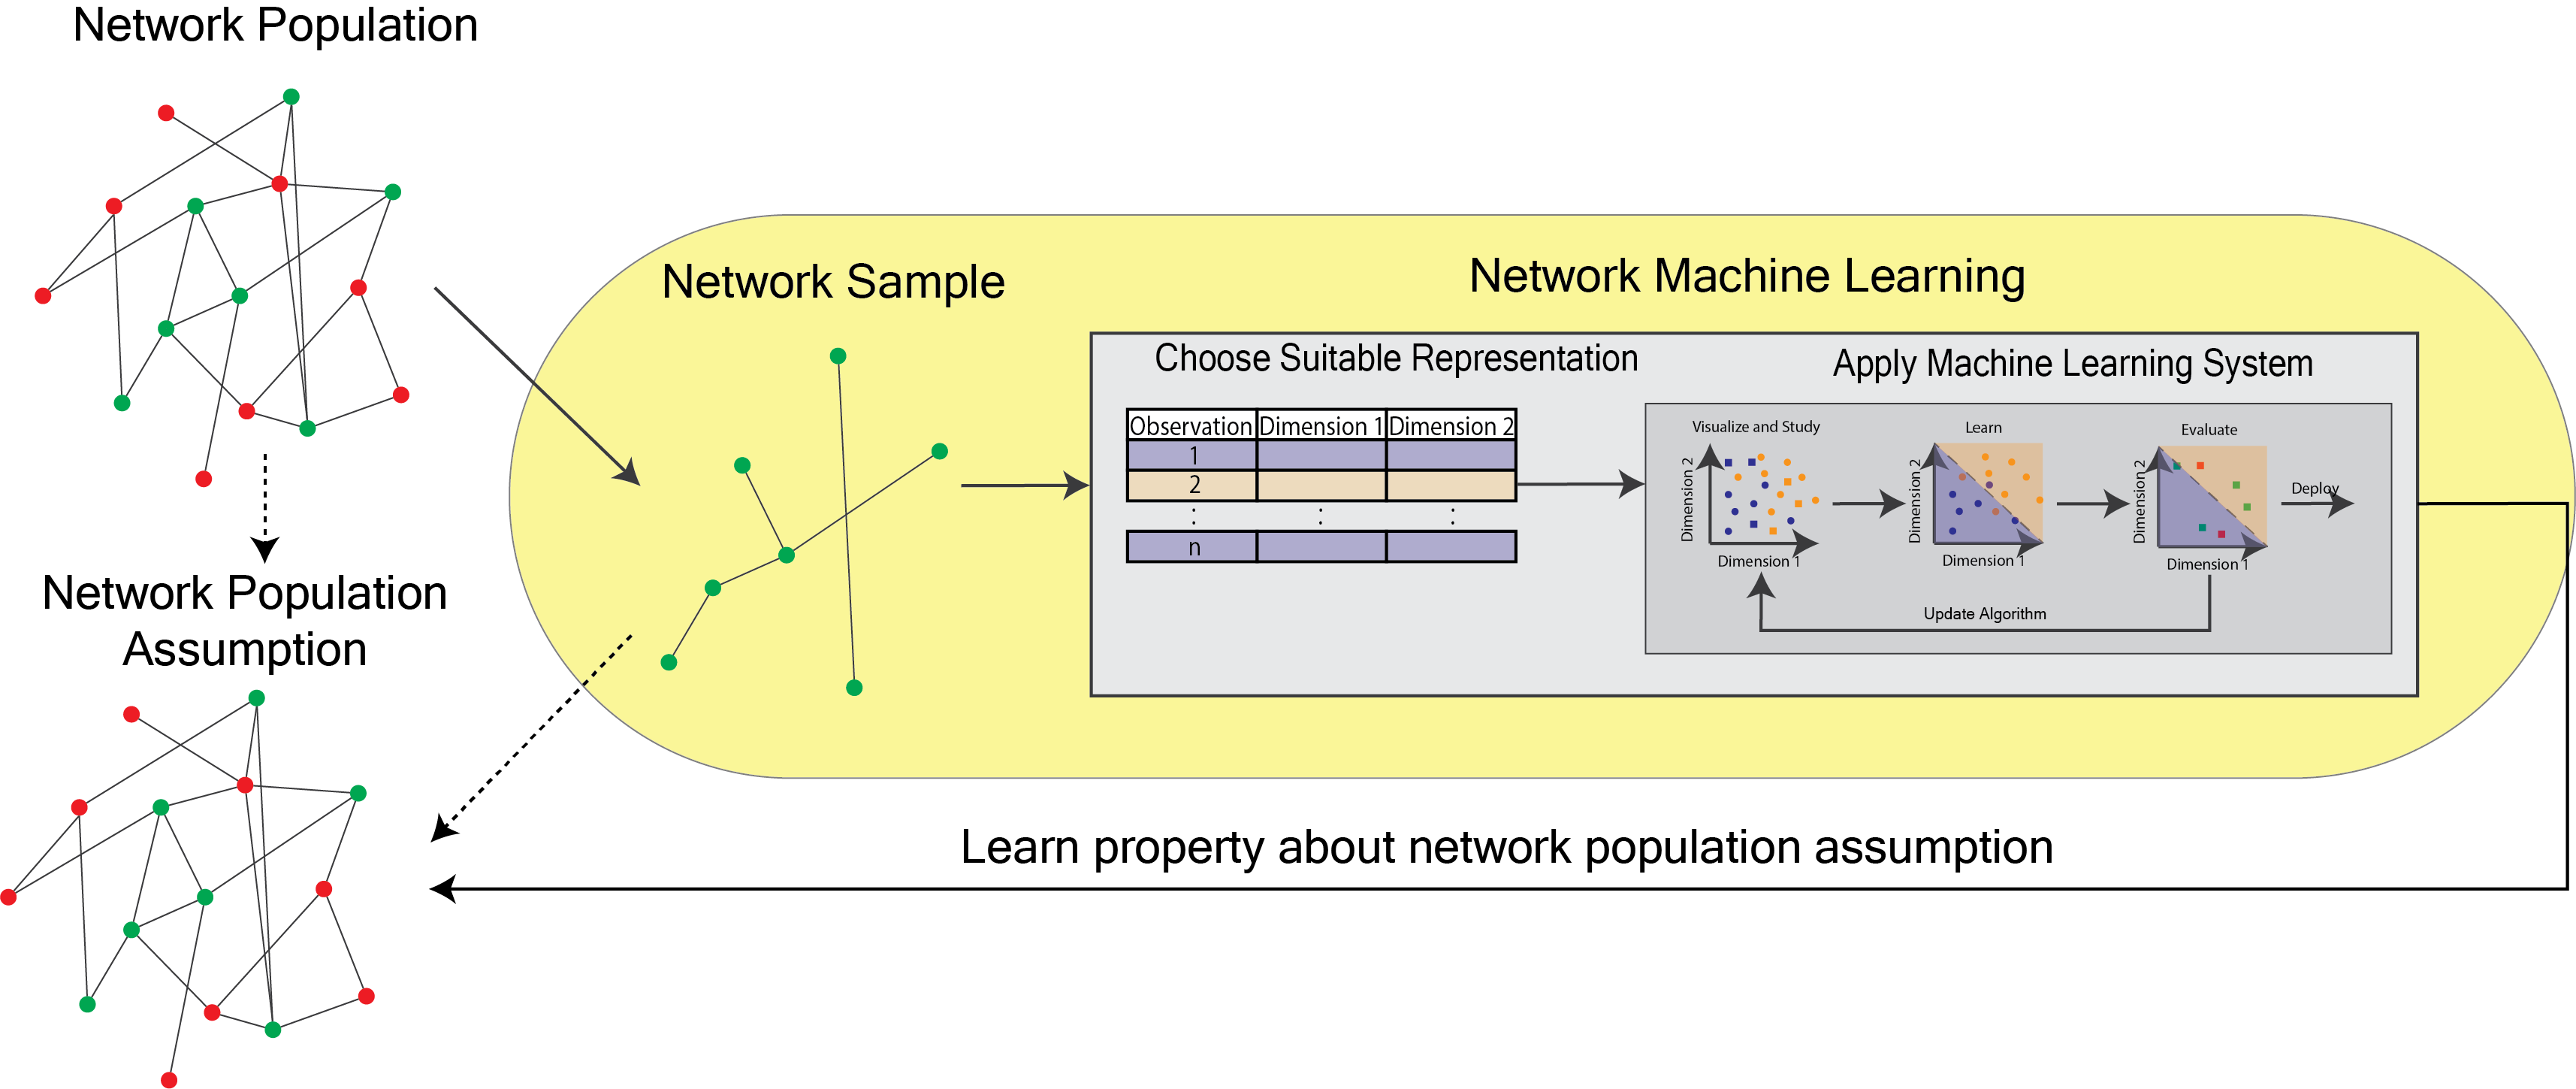
\includegraphics[width=\linewidth]{representations/ch6/Images/network_reps.png}
    \caption[Representation learning schematic]{The statistical learning pipeline. In this chapter, you will learn about how to represent networks you observe in your analysis.}
    \label{fig:ch6:netrep}
\end{figure}

It is important to note that to learn and derive useful insights from these representations, you really don't need to understand anything about the last chapter at {all}, in general. You can take the representations you learn about, apply machine learning systems to them, and then study the networks in isolation. However, these representations tend to make more intuitive sense in the context of Section \ref{sec:ch5}, and further, Section \ref{sec:ch5} provides context and assumptions in which these representations directly motivate many of the applications you will learn in Chapter \ref{sec:ch7} onwards. So, we'd recommend learning this chapter somewhat in tandem with the preceding section: as you learn a new algorithm for finding a representation of a network, go back and think about how that representation is motivated by a statistical model. This will help you understand how the pieces start to fit together as you get to the later chapters in the network machine learning landscape.

Having a complete understanding of the results in this section, and particularly, the justification for {why} we approach network representation problems in the way in which we do requires some mathematical background. For this reason, we have prepared the supplementary section Appendix \ref{app:ch13} for more advanced readers.


\section{Maximum likelihood estimation}
\label{sec:ch6:mle}

In studying network statistics, we often use single network models to represent random networks. These models are defined by certain key variables or parameters that shape the random networks they represent.

Suppose we encounter a real-world network and wish to understand it better. In doing so, we generally need to assume that this network is a specific sample of a random network characterized by certain parameters.

However, there's a catch here. This approach assumes that we already know these defining parameters, but that's not always the case. So, how do we handle this challenge?


\subsection{Erd\"os-R\'enyi (ER)}

Recall that the Erd\"os-R\'enyi (ER) random network has a single parameter: the probability of each edge existing, which we termed $p$. Thanks to the simplicity of the ER random network, we can use a method called Maximum Likelihood Estimation (MLE) to make an educated guess at what 'p' might be. For a deeper understanding of MLE, you can look at Appendix \ref{app:ch13:mle} and check out \cite{Casella2001Jun}.

Let's illustrate this concept with the familiar coin flip example.  Imagine you have a coin, but you don't know the probability of it landing on heads.  However, you're allowed to flip it 100 times and then guess the probability of it landing on heads. Let's say, after 100 flips, it landed on heads 45 times. What would be your guess for the probability of the coin landing on heads?

If you thought it might be $\frac{45}{100}$, or the number of heads you got divided by the total number of coin flips, you'd be right. This guess is the maximum likelihood estimate for a binary random variable.

The same principle applies to the ER random network. The best estimate of the probability of an edge existing in an ER random network is just the ratio of the total number of edges in the network, $m = \sum_{j > i}a_{ij}$, divided by the total number of edges possible in the network, which is $\binom n 2$.

Our result is:
\begin{align*}
    \hat p &= \frac{m}{\binom n 2}.
\end{align*}

The ``hat'' symbol ($\hat \cdot $) just means that $\hat p$ it is an \textit{estimator}: it is a function of the observed data that we use to describe the \textit{estimand}, which is the parameter of the model that we want to learn about. In this case, since we are considering an $ER_n(p)$ model, the only parameter that we want to learn about is $p$.

To bring this back to our coin flip example, this is like you are saying that there is a single coin. You flip the coin once for every possible edge between those pairs of communities, $\binom n 2$. When that coin lands on heads, that particular edge is determined to exist, and when it lands on tails, that edge does not exist. Our best guess, then, is just to count the number of heads you obtained, $m$, and divide by the number of coin flips you made, $\binom n 2$. 

Let's work on an example. You will use a sample of a random network which is ER, with $50$ nodes and an edge probability of $0.3$, similar to what we did in Section \ref{sec:ch5:er}. We begin by simulating and visualizing the appropriate network: 


\begin{lstlisting}[style=python]
from graspologic.simulations import er_np

p = 0.3
A = er_np(n=50, p=p)
\end{lstlisting}

Next, we'll fit the EREstimator model from \texttt{graspologic}, and compare the true probability $p=0.3$ to the estimated probability $\hat p$:
\begin{lstlisting}[style=python]
import numpy as np
from graspologic.models import EREstimator

model = EREstimator(directed=False, loops=False)
model.fit(A)
# obtain the estimate from the fit model
phat = model.p_
\end{lstlisting}

We can see how good the estimator performs by comparing it to the (true) population parameter, $p$:

\begin{lstlisting}[style=python]
print("Difference between phat and p: {:.3f}".format(phat - p))
\end{lstlisting}

Not bad! The estimate of the probability should end up pretty close to the true value. 

\subsection{Stochastic Block Model}

The Stochastic Block Model, like the Erdős-Rényi model, is characterized by a single parameter. However, in this case, the parameter is a block matrix, 'B'. The entries in $B$, $b_{kk'}$, denote the probabilities of edges existing between pairs of communities. 

When you apply the Maximum Likelihood Estimation (MLE) method to this model, you calculate $b_{kk'}$ by dividing $m_{kk'}$ by $n_{kk'}$. Here, $m_{kk'}$ stands for the total number of edges that actually exist between nodes in communities $k$ and $k$, while $n_{kk'}$ represents the total possible number of edges between these communities.

\begin{align*}
    \hat b_{kk'} = \frac{m_{kk'}}{n_{kk'}}.
\end{align*}

Intuitively, the estimate of the block probability $b_{kk'}$ is the ratio of how many edges you see between communities $k$ and $k'$ $m_{kk'}$ and how many edges were possible $n_{kk'}$.

To bring this back to our coin flip example, this is like saying that there is one coin $(k, k')$ for each pair of communities in our network. You flip each coin once for every possible edge between those pairs of communities, $n_{kk'}$. When that coin lands on heads, that edge exists, and when it lands on tails, that edge does not exist. Our best guess is just to count the number of heads we obtained, $m_{kk'}$, and divide by the number of coin flips we made, $n_{kk'}$. 

Remember that in the example we worked through in Section \ref{sec:ch5:sbm}, we had $100$ students, each of whom were in one of two schools (school $1$ and school $2$). If the students were both in school $1$, the probability that they were friends was $0.6$, and if the students were both in school $2$, the probability that they were friends was $0.4$. If the students attended different schools, the probability that they were friends was $0.2$. This gave us a block matrix of:
\begin{align*}
    B &= \begin{bmatrix}
        .6 & .2 \\
        .2 & .4
    \end{bmatrix}
\end{align*}

Which corresponds to a probability matrix $P$ where each entry is:
\begin{align*}
    p_{ij} &= \begin{cases}
    0.8 & i, j \leq 20 \text{ or }i, j \geq 20 \\
    0.2 & \text{otherwise}
    \end{cases}
\end{align*}

We begin by simulating an appropriate SBM:

\begin{lstlisting}[style=python]
from graspologic.simulations import sbm

n = [50, 50]
B = np.array([[0.6, 0.1], 
              [0.1, 0.4]])

A = sbm(n=n, p=B)
z = np.repeat([0, 1], repeats=[n1, n2])
\end{lstlisting}

A network sample is shown in Figure \ref{fig:ch5:sbm}.

Next, let's fit an appropriate SBM, and investigate the estimate of $B$:

\begin{lstlisting}[style=python]
from graspologic.models import SBMEstimator
from graphbook_code import heatmap

model = SBMEstimator(directed=False, loops=False)
model.fit(A, y=z)
Bhat = model.block_p_

# plot the block matrix vs estimate
heatmap(B, title=" $B$ true block matrix", vmin=0, vmax=1)
heatmap(Bhat, title="$\hat B$ estimate of block matrix", vmin=0, vmax=1)
heatmap(np.abs(Bhat - B), title="$|\hat B - B|$", vmin=0, vmax=1)
\end{lstlisting}

We investigate the difference between $B$ and $\hat B$ in Figure \ref{fig:ch6:sbm_est}.

\begin{figure}
    \centering
    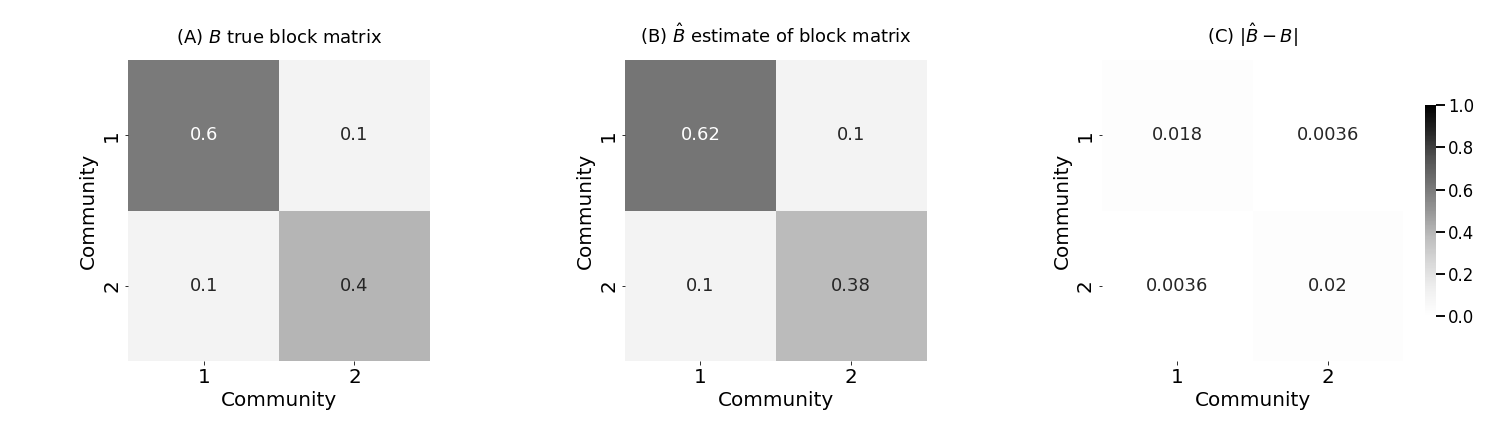
\includegraphics[width=\linewidth]{representations/ch6/Images/sbm_est.png}
    \caption[Estimating block matrix of SBM]{\textbf{(A)} the true block matrix underlying a random network. \textbf{(B)} the estimated block matrix from the network sample. \textbf{(C)} the difference between the estimated and true block matrices.}
    \label{fig:ch6:sbm_est}
\end{figure}

In this section, we've learned about estimating parameters for two types of simple networks. First, we have the $ER_n(p)$ random network. Here, edges are largely unstructured. Second, we have the $SBM_n(\vec z, B)$ network. For this, the network's structure is predetermined by known community assignments and we only need to understand 'B'.

For both types of random network, we can accurately estimate the underlying probability parameters of these models using methods like MLE.

These approaches allow us to make well-informed guesses about the likelihood of different types of connections within these networks.

\newpage
\section{Why do we embed networks?}
\label{sec:ch6:why}

We mentioned at the beginning of the chapter that a major topic of study in network machine learning is \textit{representation learning}, which deals with embedding data into modalities which we can understand as feature representations. We call these feature representations \textit{tabular data} and the way we get to it an \textit{embedding method}.

Tabular data is structured with rows representing observations and columns denoting features. This format simplifies the application of numerous ML algorithms, whether we consider neural networks, decision trees, or tasks such as classification or regression. The underlying assumption here is that each observation (row) is \textit{independent} of others, reducing complex interdependencies and correlations to simpler, feature-based relationships.

However, in network data, this independence assumption crumbles. Each node is explicitly connected to others, resulting in a web of dependencies.

Network embeddings are a way of transforming network data into a form more digestible for traditional ML algorithms. By projecting network data into a vector space (creating a 'feature representation' for each node), we retain crucial information about node relationships while also structuring the data in a way that respects the expectations of these algorithms.

There is a rich bidirectional relationship between networks and this tabular data as well. Just as we can get from networks to tabular data, we can get from tabular data to networks: for instance, for every row in our data matrix, we can define its edge weight with other rows as being some similarity metric, like Euclidean distance. Or we can binarize by taking the K nearest neighbors of a given row as its edges.

Why do we embed networks? It's a way of bridging the gap between the rich, interdependent structure of network data and the independent, feature-oriented world of traditional machine learning. It allows us to tap into the wealth of ML tools and techniques available for tabular data while still capturing the inherent complexity of networks. And it lets us view things differently, opening the door to new ways of understanding our networks.



\begin{floatingbox}[h]\caption{Lobster dataset}
To better understand the concepts of this section, we're going to go outside of network machine learning and try to understand a lobster dataset \cite{Sordalen2020Oct}. In this dataset, $n=2560$ lobsters were collected by a team of university investigators in Norway. For each lobster, the investigators measured the lobster's biological sex, the crusher claw width (CW), and the total length (TL) of the lobster, prior to release of the observed specimens (the features). Our question of interest is whether we can predict the crusher claw width using the lobster's biological sex and total length.
\end{floatingbox}

The key with this example is less the specific techniques that are applied, and more so the big picture of the implications of these problems on network data.

\subsection{Statistical dependence}

To visualize whether we might expect to find a relationship, we use a scatter plot, in Figure \ref{fig:ch5:lobster}. Each point represents the biological sex, claw width CW, and total length TL of a single lobster. There is clearly a positive association, where longer lobsters tend to have larger crusher claws. Further, it would appear that male lobsters tend to have a much more dramatic increase in crusher claw width as total length increases. This data is encoded in a tabular format, where each row indicates the observation for a single lobster, and there are three columns (crusher claw width, total length, and biological sex). 

\begin{figure}[h]
    \centering
    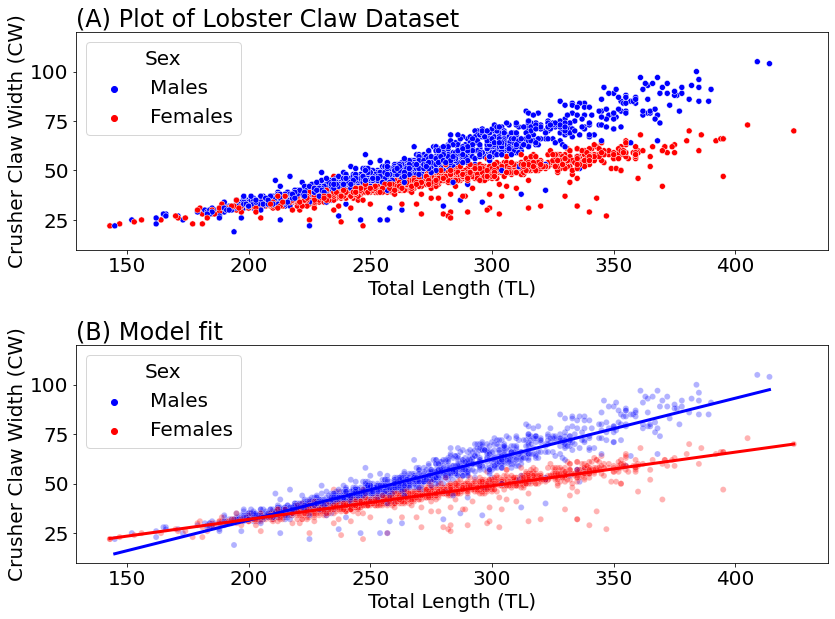
\includegraphics[width=0.7\linewidth]{representations/ch6/Images/lobster.png}
    \caption[Lobster example]{\textbf{(A)} a scatter plot of lobster total length against crusher claw width, separated by biological sex (shape). \textbf{(B)} a linear regression of the crusher claw width onto total length and biological sex, with an interaction term for biological sex and total length. Notice that the lines capture the dependence that we intuitively determined from \textbf{(A)}.}
    \label{fig:ch5:lobster}
\end{figure}


Conceptually, what this graph indicates is that there is likely a dependence in the dataset: crusher claw width appears to be related to both lobster total length (note that the larger lobsters tend to have greater claw widths) and biological sex (as males grow, their claw widths tend to increase faster than female claws).

If you remember back to traditional machine learning, it looks like you could fit a line between the total length and the crusher claw width for each lobster biological sex, and get a pretty good description of the relationship between the three features. A first-pass strategy would be to use a linear regression. In this case, based purely on the information we have gathered from visualizing the data, an appropriate model would regresses the crusher claw width onto the lobster biological sex and total length (we think that biological sex and total length are informative about crusher claw width), and allow for the biological sex to modify the relationship between total length and crusher claw width (males have a steeper increase in crusher claw width with increasing size). 

You can see the results of this regression model that we have described in Figure \ref{fig:ch5:lobster}(B). It appears as though are relatively straightforward linear regression model does a fairly good job of capturing what we can intuitively derive from visualizing the data in Figure \ref{fig:ch5:lobster}(A). In this sense, we were able to explicitly describe a dependence that we expected, model it (using linear regression), and then capture it by fitting a regression model we believed to be appropriate.

As a caveat, it is almost never this easy to study a dependence, but it is often at least {possible} to do. The key that you should pick up on is that the traditional approach to dealing with dependencies when they arise in machine learning is to model them directly (like we did above) or indirectly (using latent models, an approach we did not describe here, but you can learn about in \cite{Hastie2009}). When we have underlying dependencies in the data and want to account for them, our approach is to explicitly describe or isolate the dependence whenever possible. Further, if we are uncertain about dependencies in the model, we can often do a pretty good job of inferring them.



\subsection{Why does this simple example indicate a problem with networks?}

This example, while trivial, gives us a good sense of some of the problems we're going to run into very quickly when we try to analyze network data. 

\subsubsection*{Embedding is a tool to give you a tabular data structure}

All of the machine learning techniques and intuitions that you have probably built up through your education are most likely designed for tabular data formats. Networks are not tabular at all; an observed network is a matrix and not a vector. It is unclear how exactly you can adapt your network to allow you to learn in the tabular setting which other methods have been designed for. A network embedding is the solution to this problem, and is first and foremost a tool. Embedding is the ``bridge'' which provides functionality you need (namely, turning an adjacency matrix into a tabular format) so that you can churn them through all the other machine learning algorithms which have been developed over the years. Embedding a network and then visualizing that embedding is often low-hanging fruit to answer questions you might have about it. 

\subsubsection*{Embedding provides an intuitive bridge when considered using statistical models}

All networks have the exact type of statistical dependence which arose in the lobster data, but on a much larger scale. When studying a dataset with $2$ features there is one possible dependence that can arise: the first feature can be related to the second feature. When studying a dataset with $3$ features like above, there are three possible dependencies that can arise: the first feature being related to the second, the second related to the third, and all three being inter-related. As you build up this logic, the number of possible dependencies with $d$ features winds up being $\frac{d!}{2}$, where $d!$ is the factorial operation $d\cdot (d - 1) \cdot (d - 2) \cdot ... \cdot 1$. When $d$ is small, this is extremely manageable with explicit modelling (like we did above for the lobsters). Even when $d$ is fairly large, it's typically the case that most of these dependencies are negligible.

Unfortunately for networks, dependencies are usually explicitly non-negligible. Remember that the adjacency matrix for a network is a collection of nodes and edges. This data structure has inherent dependencies: each edge depends on a pair of nodes, so our network has {at least} $\frac{n!}{2}$ dependencies to consider when determining how to learn from it. Stated another way, any pair of nodes could be correlated (because of the edges themselves), and further, nodes could be related to one another explicitly (by a specific grouping, such as a community assignment) or implicitly (by the nodes having similarities depending on different aspects of them that aren't immediately apparent at first glance). To give you an indication of the scope of this problem, $\frac{n!}{2}$ is much bigger than $\binom n 2$, which we learned in Figure \ref{fig:ch4:nnets} is already an untenably large number even for modest choices of $n$. When $n$ is just $15$, this means there are about $10^{12}$ possible dependencies that may exist in the network.

\paragraph*{Explicitly delineating the dependence structure}

Sometimes, we can take the easy way out with network data, like we might do with tabular data: we can simply ignore a lot of the dependencies that might exist. If we think that the nodes of our network are totally unrelated, we can learn from our network by using strategies appropriate for $ER_n(p)$ random networks. Remember that the $ER_n(p)$ random network made the assumption that all pairs of nodes had an equal connection probability (namely, $p$) which did not depend on any aspect of the individual nodes themselves. 

If we are given some sort of a grouping between the nodes, such as a community assignment vector, we can learn from the network using strategies appropriate for $SBM_n(\vec z, B)$ random networks and their related cousins. Remember than the $SBM_n(\vec z, B)$ random network model made the assumption that, once you know the community assignment of a node (given by $\vec z$), the edge probability was simply the appropriate entry of the block matrix. These approaches make excellent first-passes, and can be combined with other techniques we will see arise in Part \ref{p:app}.

\paragraph*{If we can't explicitly delineate dependencies, what are we left with?}

The problem with networks that you might come across in your work is that they often won't fit into the scope of questions that you can ask with techniques that fall into this landscape where we can explicitly delineate out dependence structures immediately. 

You might have a network where you don't know a good grouping of the nodes ahead of time, or you might want to learn appropriate groupings of nodes directly from your data. You might think that there are dependencies that go beyond just a grouping of the nodes, or you might think that grouping your nodes together is inappropriate entirely. In this sense, there are a variety of ways in which prescriptive applications of SBMs with known community assignment vectors and ERs are not entirely appropriate.

 When things get more complicated is where the opportunity and excitement of network machine learning comes into play. In the next few sections, we'll start to learn a few embedding techniques.

\newpage
\section{Adjacency spectral embedding}
\label{sec:ch6:ase}

\begin{floatingbox}[h]\caption{Give $SBM_n(\vec z, B)$ random networks and linear algebra a revisit}
In this section, we're going to revisit the $SBM_n(\vec z, B)$ random networks. The intuition that you gained in \ref{sec:ch5:psd_block} will be critical for the embedding approach that we learn here, so give it another read-through if you feel unfamiliar. 

The key algorithms in this section are known as the {eigendecomposition} and the {singular value decomposition}. For a refresher on eigendecomposition, check \cite{Axler}. For singular value decomposition, read lectures 4 and 5 in \cite{Trefethen1997}.
\end{floatingbox}

Let's imagine that we have a probability matrix $P$ for a simple independent-edge random network which is positive semi-definite. Remember that for a positive semi-definite real matrix, the square-root matrix exists and is real, which we explored in Section \ref{sec:ch5:psd_block}. Since the network is simple, it's undirected, and so $P$ is symmetric.

If we let $X = \sqrt{P}$ be the square-root matrix for $P$, so that $P = X X^\top$, $P$ is the probability matrix corresponding to an $RDPG_n(X)$ random network. For our purposes, we will assume that the network has $n$ nodes, and $X$ has a latent dimensionality of $d$ which is less than the number of nodes, and that none of the columns are redundant (the rank of $X$ is $d$).

\subsection{The eigendecomposition provides us with latent position matrices for random networks with positive semi-definite probability matrices}

These facts provide us with useful information about the eigendecomposition of $P$. This information is summarized below, in Remark \ref{box:ch6:evd_sum}.

\begin{floatingbox}[h]\caption{The eigendecomposition of symmetric matrices}
\label{box:ch6:evd_sum}
Consider a real symmetric matrix $R$. The \textit{eigendecomposition} of $R$ is the factorization $R = Q\Lambda Q^\top$ where $\Lambda$ is the diagonal matrix of the ordered (in decreasing order) eigenvalues of $R$, and $Q$ is the matrix whose columns are eigenvectors of $R$. 

If $R$ is rank $d$, $\Lambda$ will have $d$ eigenvalues that are non-zero, and the remaining $n - d$ eigenvalues will be $0$. 

If $R$ is positive semi-definite, the eigenvalues will be non-negative; so, $\lambda_1 \geq \lambda_2 \geq \hdots \geq \lambda_ n \geq 0$.

Let $R$ be symmetric, positive semi-definite, and of rank $d$. We draw two important conclusions:

\begin{enumerate}
    \item The non-zero eigenvalues are ordered and positive: $\lambda_1 \geq \hdots \lambda_d > 0$.
    \item With $Q_d$ the $n \times d$ matrix whose entries are the first $d$ eigenvectors of $P$, and $\Lambda_d$ the $d \times d$ diagonal matrix whose diagonal entries are the first $d$ non-zero eigenvalues of $R$:
\begin{align*}
R = Q_d \Lambda_d Q_d^\top
\end{align*}
\end{enumerate}
Throughout this book, we notate the eigendecomposition of a matrix $R$ with $\texttt{evd}(R)$.
\end{floatingbox}

So, if $P$ is positive semi-definite, rank $d$, and symmetric, we obtain a characterization of the latent positions of $P$, where:
\begin{align*}
    P = Q_d \Lambda_d Q_d^\top = (Q_d \sqrt{\Lambda_d})(Q_d \sqrt{\Lambda_d})^\top = XX^\top,\;\;\;\; X = Q_d \sqrt{\Lambda_d}
\end{align*}
where $\sqrt{\Lambda_d}$ is the matrix whose entries are the square roots of the first $d$ eigenvalues of $P$. Note that $\sqrt{\Lambda_d}$ is real, because the top $d$ eigenvalues are positive, so their square root is defined. We can put this entire procedure together, using Algorithm \ref{alg:ch6:evd}, to obtain a latent position matrix for the random network.

\begin{algorithm}[h]\caption{Finding latent positions for a positive semi-definite probability matrix}
\label{alg:ch6:evd}
\KwData{$P$ a $n \times n$ square probability matrix which is positive semi-definite and of rank $d$.}
\KwResult{a latent position matrix for the random network.}
\SetAlgoLined
Let $Q, \Lambda = \texttt{evd}(P)$ be the eigenvectors and eigenvalues of $P$.

Let $Q_d = \begin{bmatrix}
    \uparrow & & \uparrow \\
    \vec q_1 & \hdots & \vec q_d \\
    \downarrow & & \downarrow
\end{bmatrix}$, and let $\Lambda_d = \begin{bmatrix}
    \lambda_1 & & \\
    & \ddots & \\
    & & \lambda_d
\end{bmatrix}$ be the matrix whose rows are the first $d$ eigenvectors and the diagonal matrix whose entries are the first $d$ eigenvalues of $P$.

Compute $\sqrt{\Lambda_d}$ to be the matrix whose entries are $\sqrt{\lambda_i}$, for all $i$ from $1$ to $d$.

Let $Y = Q_d \sqrt{\Lambda_d}$.

\Return{$Y$}
\end{algorithm}

This gives us a method to compute a latent position matrix for the underlying random network, which has $n$ rows (the same as the number of nodes) and $d$ columns. 

This latent position matrix $X$ is our first example of a network embedding. This matrix has $n$ rows, the same as the number of nodes in our random network. In this case we're embedding our generative model $P$, rather than an observation of it $A$, but later we'll use the same logic to embed realized networks.

Each of the $n$ rows of $X$ corresponds to a node in our network. We've embedded this network into $d$ dimensions. We'll soon see that, if we take $d$ = 2 and plot the results, networks with clear community structure embed into latent position matrices with obvious clustering structure.

\subsubsection*{Rotational non-identifiability of the latent position matrix}
\label{sec:ch6:spectral:nonidentifiable}
As it turns out, there are many ``reasonable'' latent position matrices for a random network with a positive semi-definite probability matrix, where by ``reasonable'', we mean that they all would produce the same latent position matrix. In particular, there are infinitely many embeddings that are identical up to a rotation.

A \textit{rotation matrix} $W$ in $d$ dimensions is any $d$-dimensional matrix where $WW^\top = W^\top W = I_d$, the $d$-dimensional identity matrix.

Let's imagine that $Y$ is another latent position matrix, but is a rotation of $X$. That means that there is a rotation matrix $W$ where $X = YW$. The probability matrix for the $RDPG_n(X)$ network is:
\begin{align*}
    P &= XX^\top \\
    &= YW\left(YW\right)^\top,
\end{align*}
which is because $X = YW$. Applying the definition of a transpose, we get:
\begin{align*}
    P &= YW W^\top Y^\top \\
    &= YI_d Y^\top,
\end{align*}
which is because $W$ was a rotation matrix, so $W^\top W = WW^\top = I_d$ (where $I_d$ is the rank-$d$ identity matrix). Finally, since $YI_d = Y$:
\begin{align*}
    P &= YY^\top.
\end{align*}
This shows that the $RDPG_n(Y)$ and $RDPG_n(X)$ random networks have the same probability matrices.

This is known as the \textit{rotational non-identifiability} problem with random dot product graphs, in that random networks with different latent position matrices (by as much as an arbitrary rotation by the rotation matrix $W$) can still have the same probability matrix. Therefore, different latent position matrices can describe fundamentally identical (in probability) random networks.

\subsubsection*{Limitations of the \texttt{evd} for adjacency matrices}

These results are helpful when we know the probability matrix ahead of time. In fact, we even know how to determine whether the probability matrix is positive semi-definite, using the procedure that we developed in Section \ref{sec:ch5:psd_block}, where we simply checked whether all of the eigenvalues were non-negative.


Unfortunately, in real data, we don't typically have the probability matrix; all that we have is the network itself. This network can typically be represented in an adjacency matrix. 

It would be helpful (and maybe even intuitive) if we could simply plug the adjacency matrix into Algorithm \ref{alg:ch6:evd}, and obtain a reasonable estimate of the latent positions out. Unfortunately, while this matrix is real and symmetric, it is not necessarily positive semi-definite. This means that we can't necessarily decompose it in the exact same way.

Consider, for instance, an extremely simple network:
\begin{align*}
    A &= \begin{bmatrix}
        0 & 1 \\
        1 & 0
    \end{bmatrix}
\end{align*}
Remember from \ref{sec:ch5:psd_block} that for a $2 \times 2$ matrix to be positive semi-definite, its determinant has to be strictly positive: $det(A) \geq 0$. However, $det(A) = 0 \cdot 0 - (1 \cdot 1) = -1$. This matrix is not positive semi-definite. 

This means that none of the logic leading to Algorithm \ref{alg:ch6:evd} applies to adjacency matrices; for instance, in this simple example, the matrix $\sqrt{\Lambda_d}$ is not even a real matrix (it is a complex matrix, since $\sqrt{-1} = i$). 

In practice, the implications of this trivial example are that we cannot use the eigendecomposition to obtain real estimates of latent position matrices from adjacency matrices.

\subsection{The singular value decomposition allows us to estimate embeddings}

There is a closely related approach, the \textit{singular value decomposition}, which we can use to estimate latent position matrices regardless of the positive semidefiniteness of $P$. We summarize useful results about the singular value decomposition in Remark \ref{box:ch6:svd_results}.

\begin{floatingbox}[h]\caption{The singular value decomposition of real matrices}
\label{box:ch6:svd_results}
If $R$ is a real square matrix of rank $d$, then the \textit{singular value decomposition} is the factorization $P = U\Sigma V^\top$, where $\Sigma$ is the diagonal matrix of the non-negative ordered \textit{singular values} of $P$, $U$ is an orthonormal matrix whose $n$ columns $\vec u_i$ are the $n$-dimensional \textit{left singular vectors} of $R$, and $V$ is an orthonormal matrix whose $n$ columns $\vec v_i$ are the $n$-dimensional \textit{right singular vectors} of $R$. 

If $R$ is rank $d$, $\Sigma$ will have $d$ singular values that are non-zero, and the remaining $n - d$ singular values will be $0$.

If $R$ is positive semi-definite, then all left and right singular vectors $\vec u_i = \vec v_i$ for any $\sigma_i > 0$. This implies that for positive semi-definite $R$:
\begin{align*}
    R &= U \Sigma U^\top,
\end{align*}

and so the singular value decomposition of positive semidefinite $R$ collapses into the eigendecomposition.

Further if $R$ is rank $d < n$, with $U_d$ the $n \times d$ matrix of the top $d$ left singular vectors of $U$ and $\Sigma_d$ the $d \times d$ diagonal matrix of the top $d$ singular values:
\begin{align*}
    R &= U_d \Sigma_d U_d^\top.
\end{align*}

Throughout this book, we notate the singular value decomposition of a matrix $R$ with $\texttt{svd}(R)$. 
\end{floatingbox}

This allows us to obtain a closely related characterization of the latent positions of $P$, where:
\begin{align*}
    P &= YY^\top,\;\;\;\;Y = U_d \sqrt{\Sigma_d} \numberthis \label{eqn:ch6:ase_probmtx}
\end{align*}
where $\sqrt{\Sigma_d}$ is the matrix whose entries are the square-roots of the first $d$ singular values of $P$, and $U_d$ are the first $d$ left singular vectors of $P$. 

The equality here requires the positive semi-definiteness of $P$, that $P$ is rank $d$, and that $P$ is symmetric.

However, there is a convenient caveat: the matrices $U$ and $V$ are by definition real matrices for any real matrix $R$. Further, the eigenvalues $\sigma_i$ are necessarily non-negative, which means that they have a square root which is real. This gives us a basis for the procedure in Algorithm \ref{alg:ch6:ase}. Unlike the procedure described in Algorithm \ref{alg:ch6:evd}, the procedure of Algorithm \ref{alg:ch6:ase} where $\hat Y = \texttt{ase}(A)$ will always produce a real estimate of a latent position matrix. 

\begin{algorithm}[h]\caption{Estimating latent positions from adjacency matrices (\texttt{ase})}
\label{alg:ch6:ase}
\KwData{$A$ an adjacency matrix for a simple network.\newline $d$ a target latent dimensionality.}
\KwResult{an estimate of a latent position matrix.}
\SetAlgoLined
Let $U, \Sigma, V^\top = \texttt{svd}(A)$ be the left singular vectors, the singular values, and the right singular vectors of $A$.

Let $U_d = \begin{bmatrix}
    \uparrow & & \uparrow \\
    \vec u_1 & \hdots & \vec u_d \\
    \downarrow & & \downarrow
\end{bmatrix}$, and let $\Sigma_d = \begin{bmatrix}
    \sigma_1 & & \\
    & \ddots & \\
    & & \sigma_d
\end{bmatrix}$ be the matrix whose rows are the first $d$ left singular vectors and the diagonal matrix whose entries are the first $d$ singular values of $A$.

Compute $\sqrt{\Sigma_d}$ to be the matrix whose entries are $\sqrt{\sigma_i}$, for all $i$ from $1$ to $d$.

Let $\hat Y = U_d \sqrt{\Sigma_d}$.

\Return{$\hat Y$}
\end{algorithm}

This process is known as the Adjacency Spectral Embedding, or \texttt{ase}. It is called ``Adjacency'' because it operates on the adjacency matrix. ``Spectral'' just denotes that its theoretical intuition relies on the eigenvalues/eigenvectors of $P$ (the only reason that we calculated singular values/vectors of $A$ was for the convenience that it yielded a real matrix and not a complex one, and the properties for both approaches are similar).``Embedding'' here simply means that it finds a mathematical structure contained in another (a tabular structure contained within the adjacency matrix, as explained in Remark \ref{box:ch6:tabularize}). 


\begin{floatingbox}[h]\caption{\texttt{ase} tabularizes your adjacency matrix}
\label{box:ch6:tabularize}
One of the challenges we noted in Section \ref{sec:ch1:challenges} and reiterated in Section \ref{sec:ch6:why} was that network data differs fundamentally  from traditional machine learning in that the data is not tabular. However, the embedding process has changed this for us: we have used a bag of nodes approach to tabularize the network into an real estimated latent position matrix with $n$ rows (one for each node) and $d$ columns (one for each latent dimension). This provides us with a tabular data structure, which we can build upon later on to explore the nodes using more traditional machine learning approaches. 
\end{floatingbox}


Let's make this a little more concrete with an example. Let's imagine that we have an $SBM_n(\vec z, B)$ with $100$ nodes, where the first $50$ nodes are in community $1$, and the second $50$ nodes are in community $2$. The block matrix will be homophilic, so by Section \ref{sec:ch5:psd_block}, the probability matrix is positive semi-definite.


\begin{lstlisting}[style=python]
from graspologic.simulations import sbm
from graphbook_code import generate_sbm_pmtx, lpm_from_sbm
import numpy as np

n = 100
# construct the block matrix B as described above
B = np.array([[0.6, 0.1], 
              [0.1, 0.4]])

# sample a graph from SBM_{100}(tau, B)
A, zs = sbm(n=[n//2, n//2], p=B, return_labels=True)

X = lpm_from_sbm(zs, B)
P = generate_sbm_pmtx(zs, B)
\end{lstlisting}

We show a plot of the latent positions, the probability matrix, and our network sample in Figure \ref{fig:ch6:ase:ex}. Notice that in this example, the latent positions are all equal for nodes from the same community. In light of the results we explored in Section \ref{sec:ch5:psd_block:same_lp}, this is as we would expect for an $SBM_n(\vec z, B)$ random network.

\begin{figure}
    \centering
    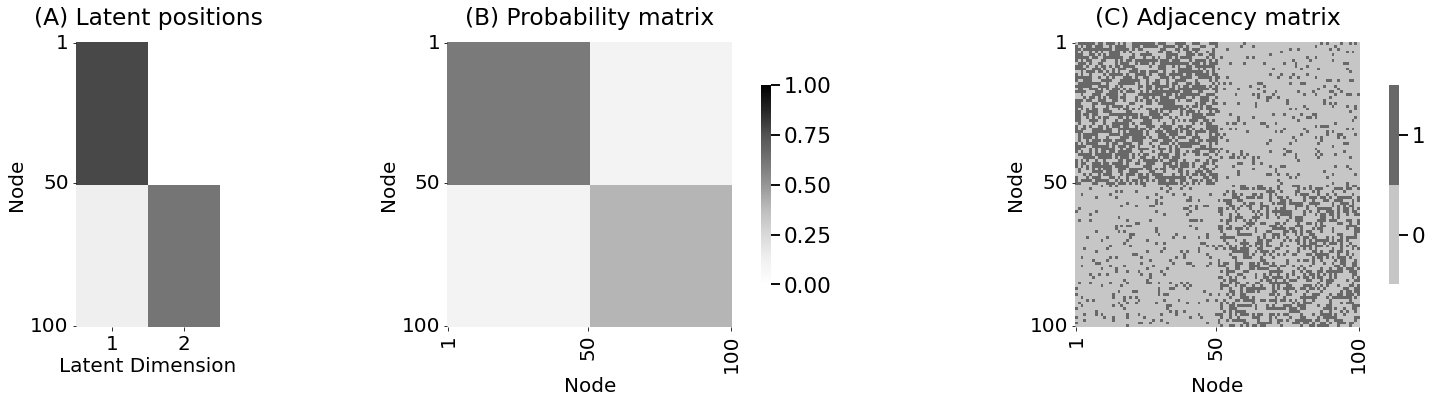
\includegraphics[width=\linewidth]{representations/ch6/Images/ase_sbm_ex.png}
    \caption[$SBM_n(\vec z, B)$ example for ASE]{\textbf{(A)} latent positions of the $SBM_n(\vec z, B)$ random network, \textbf{(B)} the probability matrix of the $SBM_n(\vec z, B)$ random network, \textbf{(C)} a sample of the $SBM_n(\vec z, B)$ random network.}
    \label{fig:ch6:ase:ex}
\end{figure}

Next, we use \texttt{graspologic} to compute the \texttt{ase} of our network sample. Note that we know that there are two communities here, so we embed into two dimensions. This gives us an estimate of the latent position matrix:

\begin{lstlisting}[style=python]
from graspologic.embed import AdjacencySpectralEmbed as ase

d = 2  # the latent dimensionality
# estimate the latent position matrix with ase
Xhat = ase(n_components=d).fit_transform(A)
\end{lstlisting}
Using this estimate of the latent position matrix, we can visualize an estimate of the probability matrix, as:
\begin{align*}
    \hat P &= \hat X \hat X^\top.
\end{align*}
Let's do this with numpy:

\begin{lstlisting}[style=python]
Phat = Xhat @ Xhat.transpose()
\end{lstlisting}
We plot the estimated latent position matrix and probability matrix in Figure \ref{fig:ch6:ase:est}(A) and (B), and the true latent position matrix and probability matrix in Figure \ref{fig:ch6:ase:est}(C) and (D).

In our example, the estimated latent positions $\hat X$ look really similar to the true latent positions $X$. However, because there is some randomness in how the \texttt{svd} algorithm is implemented in \texttt{numpy}, the non-identifiability issue that we noted in Section \ref{sec:ch6:spectral:nonidentifiable} means that your latent positions might be rotated around.

Regardless of rotational issues, you should see that the estimated probability matrix $\hat P$ should be fairly similar to the true probability matrix $P$.

\begin{figure}[h]
    \centering
    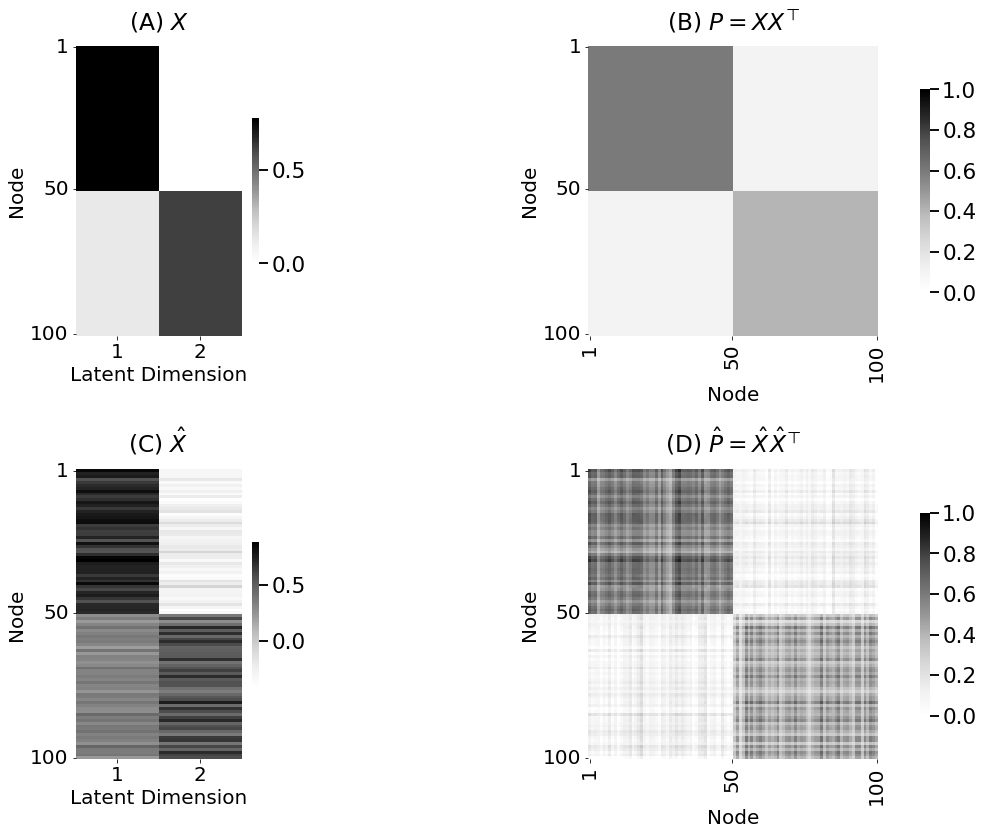
\includegraphics[width=0.7\linewidth]{representations/ch6/Images/ase_result.png}
    \caption[Comparison of ASE estimate to true prob. matrix]{\textbf{(A)} the true latent positions, \textbf{(B)} the true probability matrix, \textbf{(C)} the estimated latent positions, \textbf{(D)} the estimated probability matrix.}
    \label{fig:ch6:ase:est}
\end{figure}

Since we know the community labels of our network ahead of time, the pattern that we observe is pretty obvious. In particular, the first $50$ nodes (community $1$) tend to have similar latent position vectors, and the second $50$ nodes (community $2$) tend to have similar latent position vectors. In light of Section \ref{sec:ch5:psd_block:same_lp}, this intuitively should make sense to you: the true latent positions are {identical} for nodes in the same community, so it makes sense that the estimated latent positions will be at least close.

Now, let's consider what happens when we randomly reorder the nodes of the network, just like we did in Section \ref{sec:ch5:sbm:modularity}:

\begin{lstlisting}[style=python]
vtx_perm = np.random.choice(n, size=n, replace=False)

# reorder the adjacency matrix
Aperm = A[tuple([vtx_perm])] [:,vtx_perm]
# reorder the community assignment vector
zperm = np.array(zs)[vtx_perm]

# compute the estimated latent positions using the
# permuted adjacency matrix
Xhat_perm = ase(n_components=2).fit_transform(Aperm)
\end{lstlisting}
Now, our adjacency matrix looks like Figure \ref{fig:ch6:ase:ase_permuted}(A), and the estimated latent positions look like Figure \ref{fig:ch6:ase:ase_permuted}(B). It's not quite as obvious now that two pairs of $50$ nodes in the network have similar latent positions looking solely at the heatmap of $\hat X$ in (B), because these groups of nodes have been dispersed throughout the network. 

\begin{figure}
    \centering
    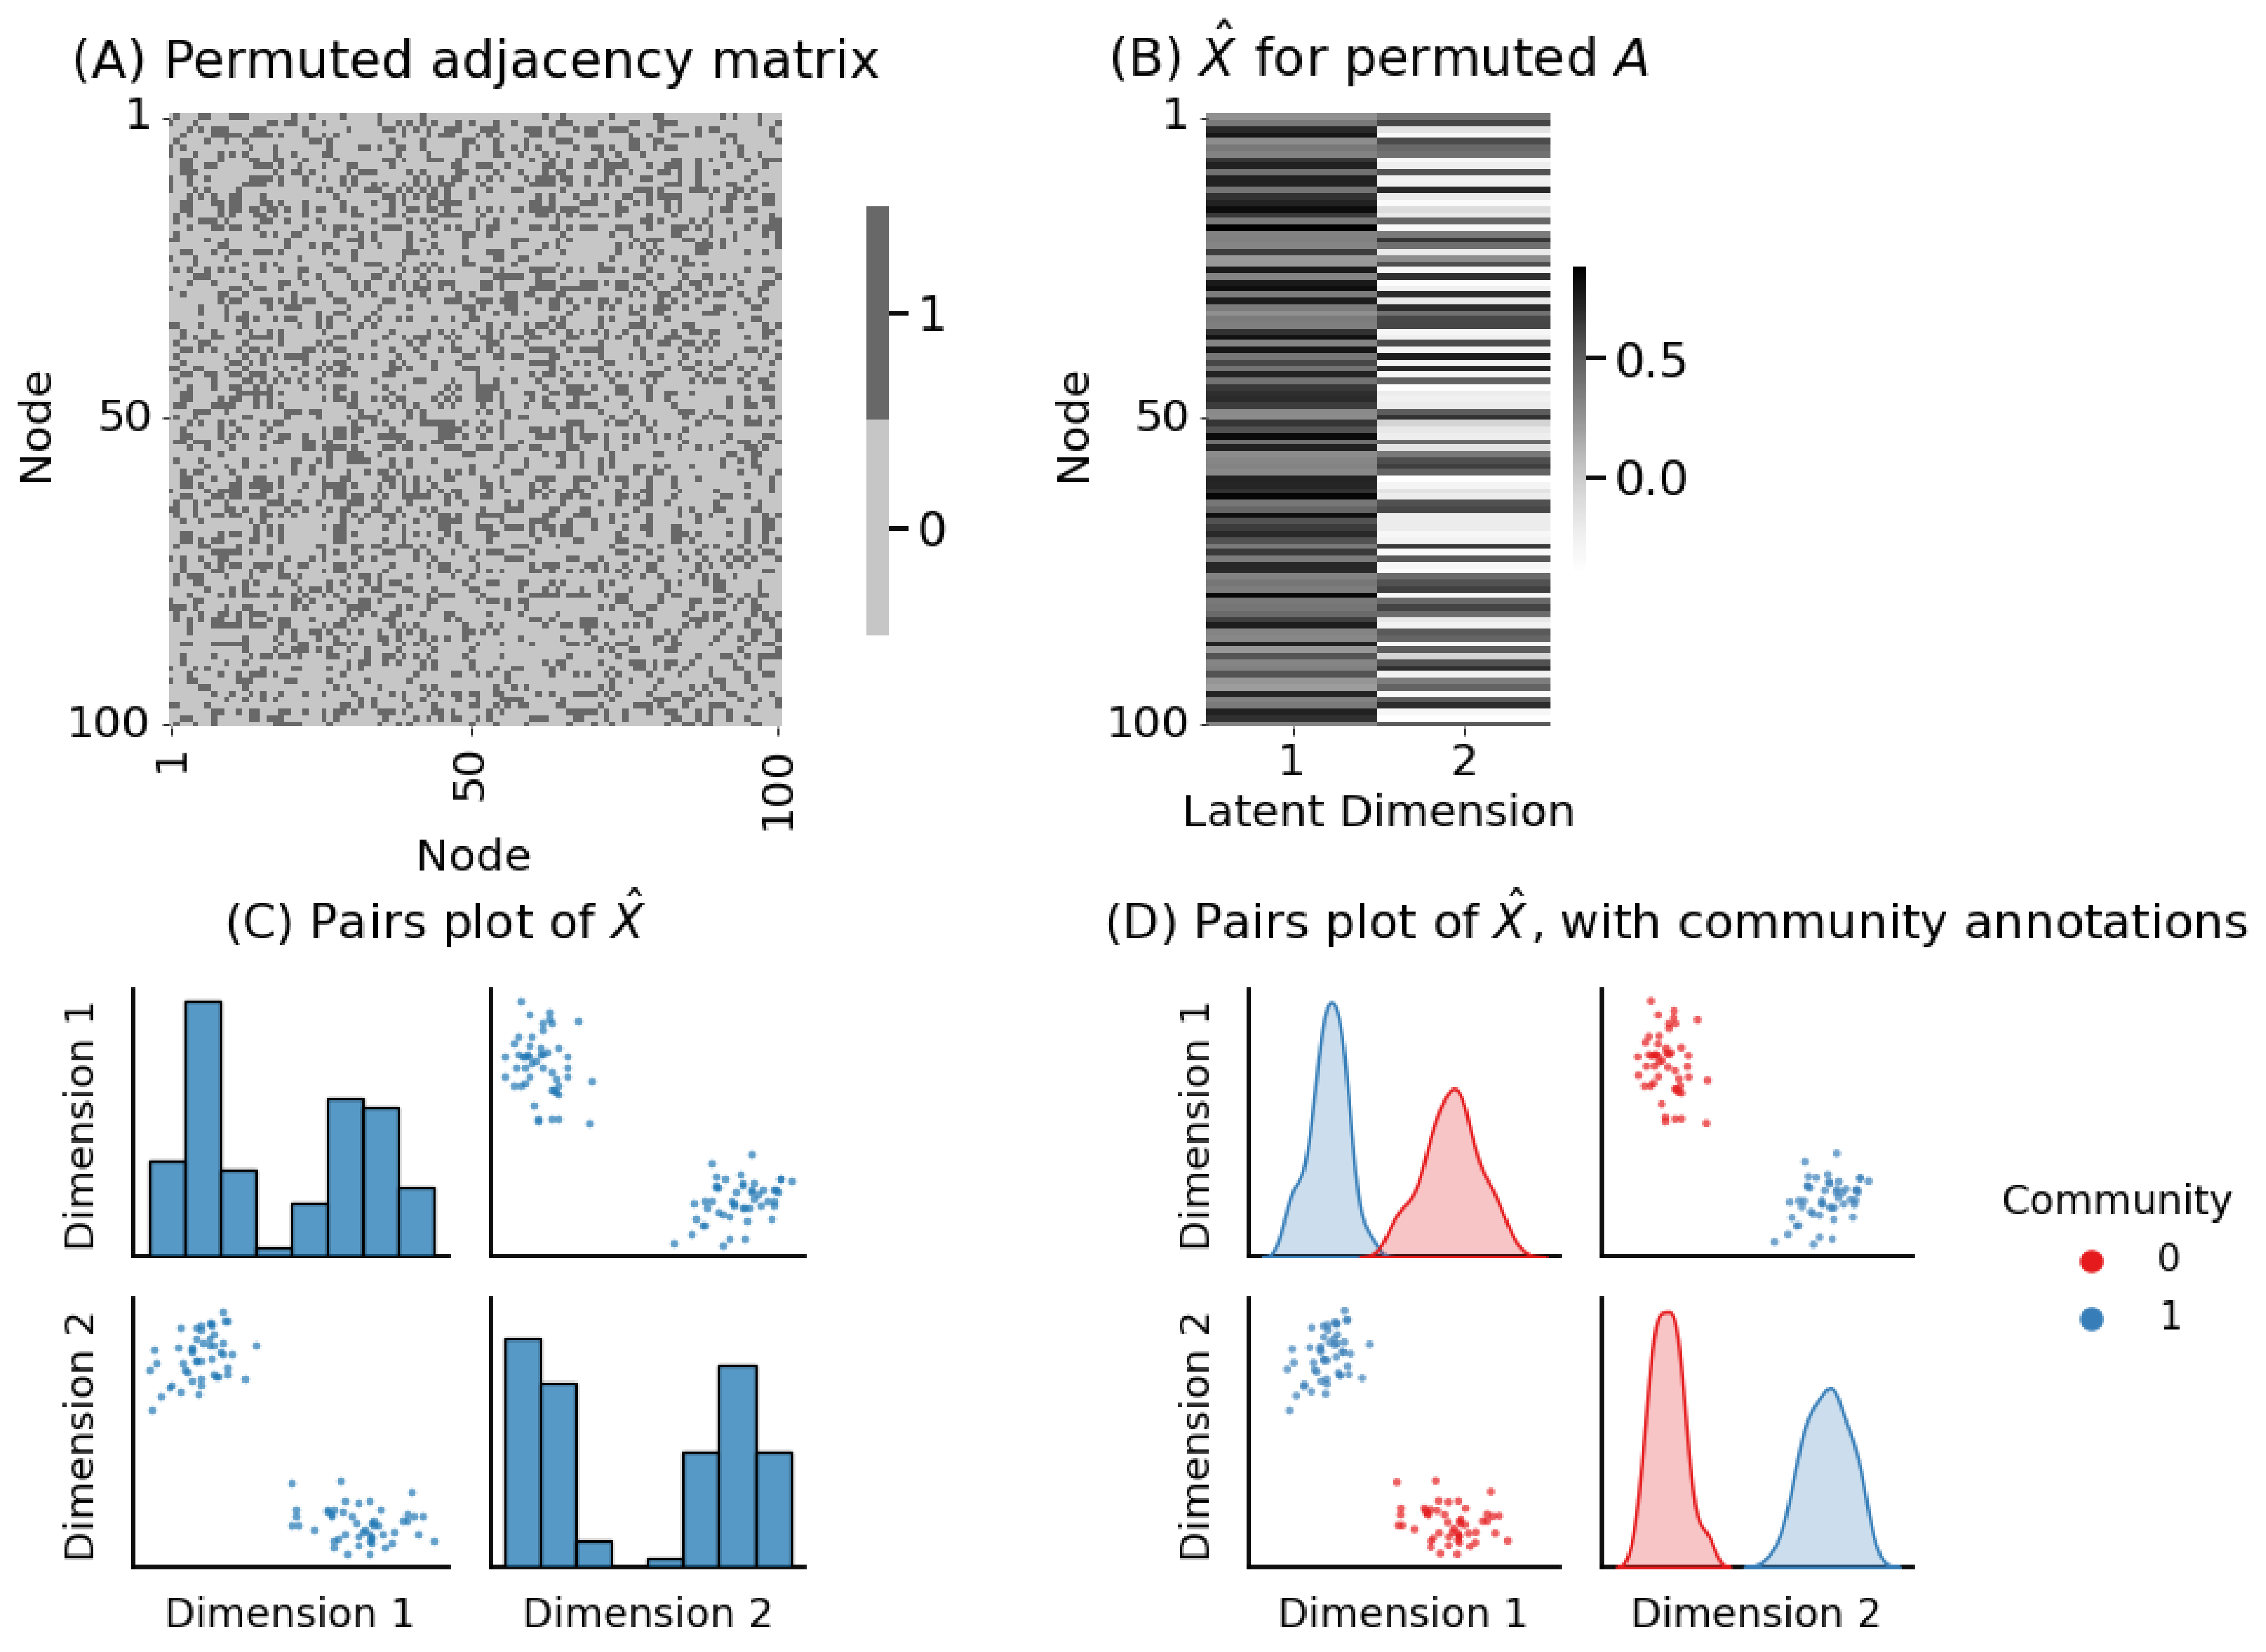
\includegraphics[width=\linewidth]{representations/ch6/Images/ase_permuted.png}
    \caption[ASE recovers latent structure, permutation-agnostic]{\textbf{(A)} the permuted adjacency matrix, \textbf{(B)} the estimated latent positions of the permuted adjacency matrix. \textbf{(C)} the pairs plot of the estimated latent positions of the permuted adjacency matrix, and \textbf{(D)} the pairs plot shown with the true community labels of the nodes.}
    \label{fig:ch6:ase:ase_permuted}
\end{figure}

\subsubsection*{The ``pairs plot'' for estimated latent positions}
\label{sec:ch6:ase:reorder}
One way to visualize tabular data structures is to use something called a ``pairs plot''. With a pairs plot, you visually investigate tabular data for \textit{latent structure}; that is, you to look for patterns that are hidden in a dataset.

To study the pairs plot, you can simply call the pairs plotting utility directly from graspologic:

\begin{lstlisting}[style=python]
from graspologic.plot import pairplot

fig = pairplot(Xhat, title="Pairs plot of $\hat X$")
\end{lstlisting}

The pairs plot for the estimated latent positions is shown in Figure \ref{fig:ch6:ase:ase_permuted}(C). The pairs plot is a d x d matrix of plots, where d is the total number of features of the matrix for which a pairs plot is being produced. The plot is called a ``pairs'' plot because it plots “pairs” of dimensions. Notice that there are two distinct looking ``blobs'' of point clouds in the pairs plot of $\hat X$.

For each off-diagonal plot (the scatter plots), the $k^{th}$ row and $l^{th}$ column scatter plot has the points $(x_{ik}, x_{il})$ for each node in the network. Stated another way, the off-diagonal plot is a scatter plot for each node of the $k^{th}$ dimension and the $l^{th}$ dimension of the matrix being plotted. That these scatter plots indicate that the points appear to be separated into individual clusters provides evidence that there might be latent community structure in the network. It is pretty clear that this plot is symmetric, since the off-diagonal entries are simply mirror images of one another (one will be dimension $k$ against dimension $l$, and the off-diagonal entry will be dimension $l$ against dimension $k$).

The diagonal elements of the pairs plot simply represent histograms or density estimates (called \textit{Kernel Density Estimates}, or KDEs) of the estimated latent positions for each dimension. If you do not pass in labels, you obtain histograms, which are just scaled bins which show the number of points for a given dimension which fall into the indicated range. If you do pass in labels, you obtain density estimates, where higher densities indicate that more points have latent position estimates in that range. For instance, the top-left density estimate indicates a density estimate of the first latent dimension for all nodes, the middle is a density estimate of the second latent dimension for all nodes, so on and so forth.

When the number of embedding dimensions is two, showing a full pairs plot is redundant, so we will often simply show a scatter plot of dimension $1$ against dimension $2$ for two-dimensional settings.

Now, let's see what happens to the pairs plot for $\hat X$, which we pass in the community labels for the nodes:

\begin{lstlisting}[style=python]
fig = pairplot(Xhat_perm, labels=zperm, legend_name = "Community",
             title="Pairs plot of randomly reordered $\\hat X$")
\end{lstlisting}

The resulting plot is shown in Figure \ref{fig:ch6:ase:ase_permuted}(D). Now we're getting somewhere! It looks like these two distinct ``blobs'' that we noticed in (C) each correspond to a single community in the underlying $SBM_n(\vec z, B)$ random network. In fact, nodes of the same community will tend to have estimated latent positions that are close together. When we say the vectors are ``close together'', what we really are talking about is with respect to the Euclidean distance. The Euclidean distance is defined in Concept \ref{def:ch6:se:eucl_dist}.

\begin{floatingbox}[h]\caption{Concept: Euclidean distance between two vectors}
\label{def:ch6:se:eucl_dist}

If $\vec x = (x_i)_{i = 1}^d$ and $\vec y = (y_i)_{i = 1}^d$ are two $d$-dimensional real vectors, the \textit{Euclidean distance} is defined as:
\begin{align*}
    d(\vec x, \vec y) = \|\vec x - \vec y\|_2 = \sqrt{\sum_{i = 1}^d (x_i - y_i)^2}.
\end{align*}
\end{floatingbox}
To evaluate this, we can compute the distance matrix of the estimated latent positions, $D$. We'll rotate back to the unpermuted points for this plot, just to make the intuitive connection more immediate. Each entry $D_{ij}$ corresponds to the distance $d(\hat{\vec x}_i, \hat{\vec x}_j)$ between all pairs of estimated latent positions. We can compute the pairwise distance matrix using \texttt{scipy}:

\begin{lstlisting}[style=python]
from scipy.spatial import distance_matrix

D = distance_matrix(Xhat, Xhat)
\end{lstlisting}
A plot of the pairwise distance matrix is shown in Figure \ref{fig:ch6:ase:nonidentifiable}(A). Note that the pairwise distance matrices between the first $50$ nodes (community $1$, the upper-left block of the pairwise distance matrix) and the second $50$ nodes (community $2$, the bottom-right block of the pairwise distance matrix) are relatively small, but the pairwise distances between nodes from community $1$ and nodes from community $2$ (and vice-versa, in the upper-right and bottom-left blocks of the pairwise distance matrix) are relatively large.

This will be extremely useful to us in Section \ref{sec:ch7:comm_detect} when we attempt to estimate underlying community structure from $SBM_n(\vec z, B)$ random networks.

\subsubsection{Rotational non-identifiability and the estimated latent positions}

As we mentioned in Section \ref{sec:ch6:spectral:nonidentifiable}, the latent positions are rotationally non-identifiable, in that for an $RDPG_n(X)$ with latent positions $X$, an $RDPG_n(XW)$ where $W$ is a $d$-dimensional rotation matrix has the same probability matrix. The estimated latent positions $\hat X$ share this issue. Now that we have estimated latent positions, we can illustrate this with our example. 

Let's see what our original latent positions look like as a scatter plot (a plot of $\hat X$ similar to the pairs plot you learned about above), and then when we apply a rotation matrix $W$ to $\hat X$, such as if we rotate $\hat X$ by $90^\circ$ to the right:

\begin{lstlisting}[style=python]
# a rotation by 90 degrees
W = np.array([[0, 1], [1, 0]])
Yhat = Xhat @ W

np.allclose(Yhat @ Yhat.transpose(), Xhat @ Xhat.transpose())
# returns True
\end{lstlisting}

As you can see in Figure \ref{fig:ch6:ase:nonidentifiable}, the estimated latent positions in (B) are basically the same in (C), except they are rotated by $90^\circ$ to the right. Note that the top blob has moved to the right, and the right blob has moved to the bottom. This is one particular example of a rotation, but there are infinitely many rotations we could make for our $2$-dimensional latent position matrix.

\begin{figure}[h]
    \centering
    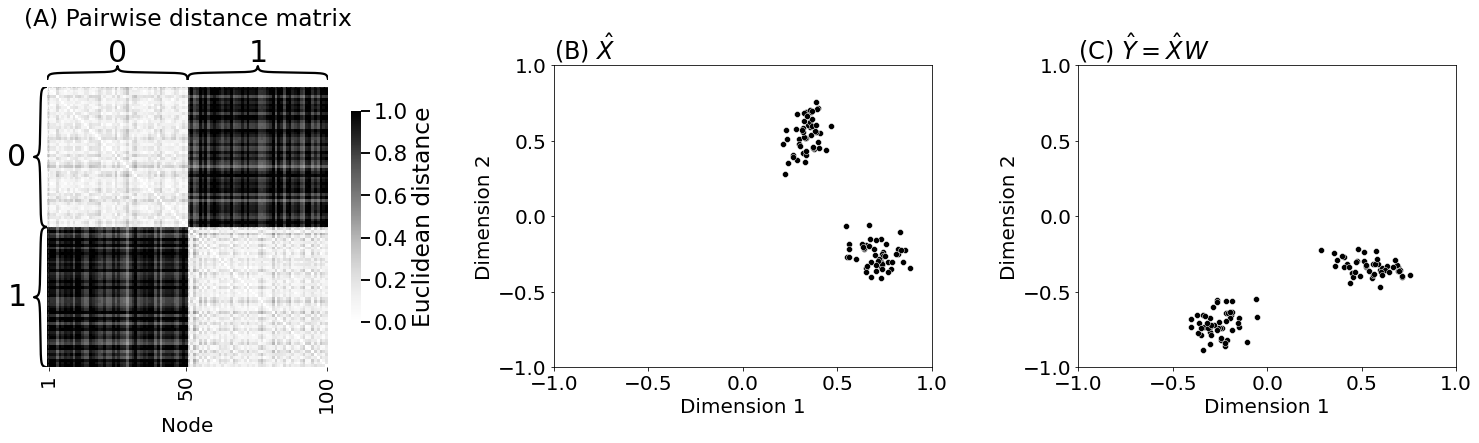
\includegraphics[width=\linewidth]{representations/ch6/Images/rotation.png}
    \caption[Pairwise distance matrices for latent positions]{\textbf{(A)} the pairwise distance matrix between the latent position vectors of all pairs of nodes, \textbf{(B)} the estimated latent positions, \textbf{(C)} the estimated latent positions, but rotated by $90^\circ$.}
    \label{fig:ch6:ase:nonidentifiable}
\end{figure}


\subsection{Why do we use \texttt{ase}?}
\label{sec:ch6:ase:whyuse}
At a very high level, the utility of \texttt{ase} is that it tabularizes your adjacency matrix, into an $n \times d$ real matrix, where $d$ was the number of dimensions that you selected to embed into. This provides the utility that you can learn about the nodes of your network via traditional machine learning approaches by treating the rows of the resulting matrix $\hat X$ as observations, and the columns of the matrix $\hat X$ as features. 

By now, we are ready to explore at a high level three additional reasons that we turn to \texttt{ase}:

\paragraph*{It always finds the latent positions for the probability matrix, given the latent dimensionality}

If you conceptualize your network sample as being a sample from an $IER_n(P)$ random network where the probability matrix is positive semi-definite, the procedure that you are using on the adjacency matrix is the same procedure that could operate on the underlying probability matrix and find the latent positions of it exactly (up to a rotation). \texttt{ase} was able to do this even if the underlying matrix was not positive semi-definite, so we would always obtain a real matrix (when we use something like an adjacency matrix).

\paragraph*{\texttt{ase} decouples the dependencies of the random network}

Studying $Y$ is equivalent (statistically) to studying $P$ when $P$ is a function of $Y$, such as $P = YY^\top$. Since $Y$ is far simpler than $P$ (it will usually have fewer columns, in practice), it will be easier to study, too.

Remember that a major limitation that we mentioned in Section \ref{sec:ch6:why} was that, for a random network $\mathbf A$, the dependency structure was simply too complicated to think about. This was because edges of the network were inherently coupled to the nodes of the network, suggesting that there were a number of possible dependencies on the order of $\frac{n!}{2}$ in the network (which was a really big number).

The probability matrix $P$ determines the structure of the random network $\mathbf A$, so we can study the probability matrix $P$ to gain insights about the dependencies in $\mathbf A$. If $P$ is positive semi-definite and $P = YY^\top$ for a set of latent positions, it is the case that the dependency structure encoded by $P$ is also encoded by $Y$. This means that the latent positions, which often will have a number of columns that is less than the number of nodes, encode the complicated dependency structure of the underlying network.

If the number of latent dimensions is less than the number of nodes in the network, that the number of possible dependencies that we will have to explore will be far less when we study the latent positions than when we study the random network (via the probability matrix) itself. 

\paragraph*{Estimated latent positions from \texttt{ase} are directly related to latent positions of random networks}

Most of the details that we have we have used thus far to conceptualize \texttt{ase} as a reasonable strategy deal with the spectral embedding of the probability matrix $P$, and the true underlying latent positions of the probability matrix (up to a rotation). We don't have this matrix $P$ in practice; we only have $A$. 

As long as we are comfortable with assuming that $A$ is a sample from a random network $\mathbf A$ with probability matrix $P$, there is theoretical reason to do this, too. ``Assuming that $A$ is a sample from a random network $\mathbf A$'' very loosely means that it makes sense to think that there was some level of randomness to the network sample. In light of the fact that most network samples are imperfect, which we explored in Section \ref{sec:ch1:howstudy}, this is not a major conceptual stretch to make.

Under this assumption, the estimates of latent positions $\hat Y$ will closely approximate the true latent positions $Y$ (up to a rotation) of $\mathbf A$ as the number of nodes in the network increases \cite{Sussman2012Sep,Athreya2017Jan,Rubin2022Sep}, and the estimate of the probability matrix $\hat P$ will closely approximate the true probability matrix $P$ (with no qualifications needed about rotations, due to the potential rotation of $\hat Y$ being ``cancelled out'' when we compute the probability matrix, like we saw in Section \ref{sec:ch6:spectral:nonidentifiable}). This is good news for us; it makes intuitive sense for estimates to be better and better approximates (on average) of the things they are approximating when we see more and more data. The theoretical advantages of \texttt{ase} are studied in detail in Appendix \ref{app:ch13:spectral}. 

There is an asterisk that will come up in a particular set of problems in which this does not hold, known as sparse networks, which will be discussed in Section \ref{sec:ch7:sparse}.

In the context of your work, what this means is that if conceptualizing your network as a sample of a random network with a positive semi-definite probability matrix feels appropriate, studying $\hat Y$ will be a good surrogate to use in place of studying $Y$ (since you can't obtain $Y$ from a network adjacency matrix $A$). This is powerful because the set of $IER_n(P)$ random networks where the probability matrix is positive semi-definite include many complicated structures, such as those shown in Section \ref{sec:ch5:psd_block}, and extensions of these structures to more than two communities. In fact, even outside of positive semi-definite structures, \texttt{ase} is still a reasonable strategy as we discuss briefly in Section \ref{sec:ch6:dimest:grdpg}. This approach therefore generalizes readily to a plethora of network learning problems. 

\subsection{Linear Algebra Considerations}

There is a lot of linear algebra that can help you build the intuition that you need to understand Remarks \ref{box:ch6:evd_sum} and \ref{box:ch6:svd_results}. We pulled this into Appendix \ref{app:ch13:ase}.

\newpage
\section{Laplacian spectral embedding}
\label{sec:ch6:lse}

Last section, we covered a lot of fascinating results. We learned that adjacency spectral embedding, or \texttt{ase}, could be used to learn useful estimates of the latent positions (up to a rotation) for positive semi-definite probability matrices. We observed that estimated latent positions for nodes in the same community of a $SBM_n(\vec z, B)$ random network where $B$ was homophilic (and hence, positive semi-definite, by Section \ref{sec:ch5:psd_block:homophily}) tended to be similar. 

The reason that the latent positions for nodes in the same community are similar boils down to our observation from Section \ref{sec:ch5:psd_block:same_lp}, that the latent positions for nodes of the same community were identical. As we mentioned briefly in Section \ref{sec:ch6:ase:whyuse}, the estimated latent position matrix produced by \texttt{ase} is going to reasonably estimate the latent positions of the underlying random network. Therefore, in some sense by transitivity (and in a literal sense, by rigorous theory from \cite{Athreya2017Jan} that is overviewed in Appendix \ref{app:ch13:spectral}), the estimated latent positions for nodes from the same community will be almost identical.

Unfortunately, many networks don't really make sense to conceptualize as $SBM_n(\vec z, B)$ random networks. Remember that an overarching assumption of $SBM_n(\vec z, B)$ random networks was that the probability for a pair of nodes $i$ and $j$ being connected depended only on their community assignments $z_i$ and $z_j$, and this probability was given by the block matrix entry $b_{z_i z_j}$ in Section \ref{sec:ch5:sbm}. This is fairly limiting, in that actual characteristics of the node itself (such as the node's popularity, or degree-correction factor) are irrelevant.

\subsection{Estimates of latent positions do not necessarily preserve within-community similarity for $DCSBM_n(\vec z, \vec \theta, B)$ random networks}

For the reasons we just touched on, an often used conceptual model for real networks are the $DCSBM_n(\vec z, \vec \theta, B)$ random networks. It might be natural to expect that, perhaps, nodes from a sample of a $DCSBM_n(\vec z, \vec \theta, B)$ random network that is positive semi-definite will share the pattern we noticed with $SBM_n(\vec z, B)$ random networks: their estimated latent positions will be similar if they are in the same community. 

This intuition is fairly close, but not quite correct. From Section \ref{sec:ch5:psd_block:same_lp}, remember that the latent positions for nodes of the same community in a $DCSBM_n(\vec z, \vec \theta, B)$ random network are identical up to a rescaling by the nodes' degree-correction factors $\theta_i$ and $\theta_j$. 

In the same notation that we used in \ref{sec:ch5:psd_block:same_lp}, the latent position vectors for a $DCSBM_n(\vec z, \vec \theta, B)$ random network were:
\begin{align*}
    \vec x_i^\top &= \theta_i \vec c_i^\top B 
\end{align*}
where $\vec c_i$ is a column-vector corresponding to the $i^{th}$ row of the one-hot-encoding of the community assignment vector $\vec z$. That is, $c_{ik} = 1$ when $z_i = k$, and $0$ otherwise. Geometrically, $\theta_i$ is ``rescaling'' the vector $\vec c_i^\top B$, where the vector $\vec c_i^\top B$ is the same for the entire community.

We can make this a little more concrete with an example. Let's use a similar same $DCSBM_n(\vec z, \vec \theta, B)$ example that we used in Section \ref{sec:ch5:dcsbm}, but make the degree-correction factors $\vec \theta$ a little more extreme:

\begin{lstlisting}[style=python]
import numpy as np
from graphbook_code import dcsbm

nk = 50  # 50 students per school
z = np.array([1 for i in range(nk)] + [2 for i in range(nk)])
B = np.array([[0.6, 0.2], [0.2, 0.4]])  # same probabilities as from SBM section
theta = np.tile(10**np.linspace(0, -1, nk), 2)
A = dcsbm(z, theta, B)
\end{lstlisting}
Next, we compute the \texttt{ase} of $A$, using the same strategy from Section \ref{sec:ch6:ase}, and we compute a pairwise distance matrix:

\begin{lstlisting}[style=python]
from graspologic.embed import AdjacencySpectralEmbed as ase
from scipy.spatial import distance_matrix

d = 2  # the latent dimensionality
# estimate the latent position matrix with ase
Xhat = ase(n_components=d).fit_transform(A)
# compute the distance matrix
D = distance_matrix(Xhat, Xhat)
\end{lstlisting}

Figure \ref{fig:ch6:lse:dcsbm_ase}(A) shows a scatter plot of the estimated latent positions, annotated with the community of each node (color; red is community $1$, and blue is community $2$). Note that the estimated latent positions appear to be ``elongated'' blobs for a given community. When we say ``elongated'', we mean that the blobs are elliptical, where the red blob elongates towards the upper-right, and the blue blob elongates towards the lower-right in our figure.

\begin{figure}
    \centering
    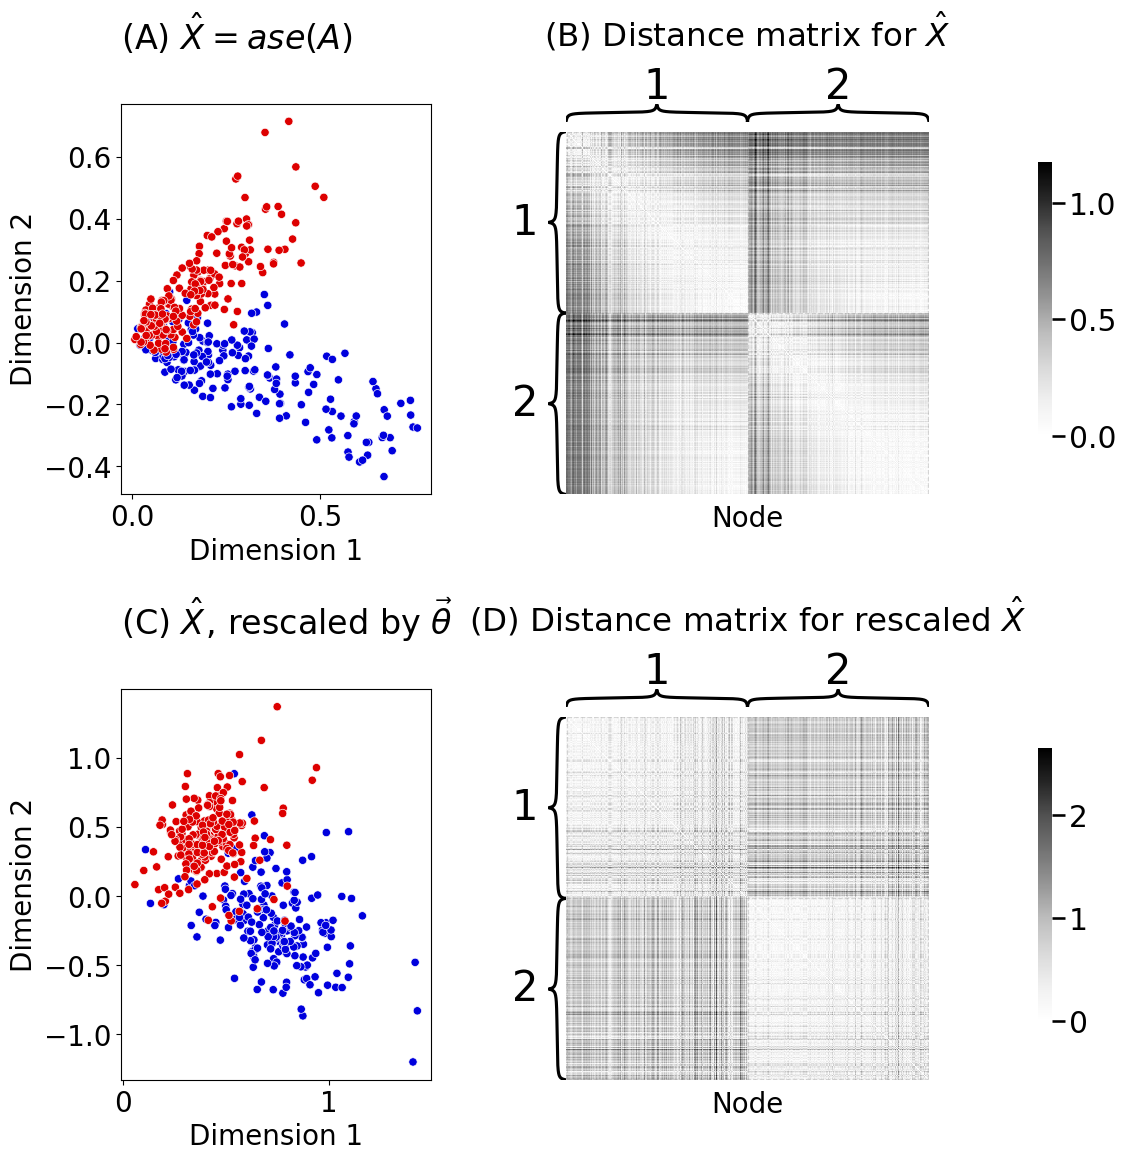
\includegraphics[width=0.8\linewidth]{representations/ch6/Images/dcsbm_ase.png}
    \caption[LSE exmaple on DCSBM]{\textbf{(A)} the estimated latent positions for a network sample of a $DCSBM_n(\vec z, \vec\theta, B)$ random network, and \textbf{(B)} the pairwise distance matrix.}
    \label{fig:ch6:lse:dcsbm_ase}
\end{figure}
We can understand this because the true latent positions for each node $i$ are given by $\vec x_i = \theta_i B\vec c_i^\top$, where $\vec c_i$ is a vector whose value $c_{ik} = 1$ if $z_i = k$, and $0$ otherwise. In this sense, the true latent positions are ``stretched'' by the degree-correction factors. Using an informal transitivity argument, the estimated latent positions are estimating the true latent positions which are stretched along an axis, so the estimated latent positions will also end up stretched along an axis. 

As indicated in the distance matrix in Figure \ref{fig:ch6:lse:dcsbm_ase}(B), this results in the distance matrix for nodes in the same community generally being pretty similar, but there are a lot of nodes where the distances across community are smaller than the within-community distances. This is indicated by the dark gray bands in the distance matrix in the upper-left and lower-right blocks of the distance matrix, as well as the light gray bands in the upper-right and lower-left blocks of the distance matrix.

Next, let's see what happens when we divide each latent position by the underlying degree-correction factor. The rows of \texttt{Xhat\_rescaled} consist of the entries $\frac{\hat{ \vec x}_i^\top}{\theta_i}$, so we have basically ``unstretched'' each latent position by the degree-correction factor:

\begin{lstlisting}[style=python]
Xhat_rescaled = Xhat / theta[:,None]
D_rescaled = distance_matrix(Xhat, Xhat)
\end{lstlisting}
These rescaled latent positions are shown in Figure \ref{fig:ch6:lse:dcsbm_ase}(C), and the pairwise distance matrix is shown in Figure \ref{fig:ch6:lse:dcsbm_ase}(D). Notice that rescaling by the degree-correction factors $\theta_i$ eliminated this ``stretching'' effect in the estimated latent positions. Further, the distances are now virtually devoid of the cross-community similarity: we are back to nodes of the same community having generally smaller distances that pairs of nodes in opposite communities.

This suggests that the degree-correction vector $\vec\theta$ can be used in conjunction with \texttt{ase} to recover rescaled latent positions where, after rescaling, the rescaled latent positions for nodes in the same community tend to be close together (in terms of the Euclidean distance).

The problem in practice is that we don't have the degree-correction vector; the degree-correction factor was a parameter of the random network, and we only have a sample $A$ of the random network.

\subsection{The Laplacian Spectral Embedding preserves within-community similarities for positive semi-definite block matrices with degree-corrections}

Remember that we obtained that if $P$ was positive semi-definite, that $\texttt{ase}(P)$ gave us two matrices $U_d$ and $\Sigma_d$, where:
\begin{align*}
    P &= XX^\top,
\end{align*}
where $X = U_d\Sigma_d$ was the latent position matrix (up to a rotation) for the random network. When we instead used an adjacency matrix, we obtained that $\texttt{ase}(A)$ gave us two matrices $U_d$ and $\Sigma_d$

As it turns out, this procedure that we described also works for functions of the probability matrix that preserve positive semi-definiteness. One very interesting function would be multiplying by diagonal matrices that only take positive real values. If a matrix $R$ is positive semi-definite, and a matrix $D$ is diagonal with only positive values, then both $DR$ and $RD$ are also positive semi-definite. In Remark \ref{box:ch6:exp_deg}, we'll re-introduce one such matrix that we've seen already.

\subsubsection{The population network laplacian}
\label{sec:ch6:lse:props}

In section \ref{sec:ch5:prop:poplapl}, we introduced the population network Laplacian $\mathcal L$. We defined it as:
\begin{align*}
    \mathcal L &= \mathcal D^{-\frac{1}{2}}P \mathcal D^{-\frac{1}{2}}.
\end{align*}
The diagonal matrix $\mathcal D$ was the expected degree matrix, with diagonal entries $\mathbb E[\mathbf d_i]$ were the expected degrees of each of the nodes in the network. Assuming that every node $i$ had at least one other node $j$ where $p_{ij} > 0$, the diagonal entries are positive, and the inverse square-root matrix $\mathcal D^{-\frac{1}{2}}$ was just the diagonal matrix with entries $\frac{1}{\sqrt{\mathbb E[\mathbf d_i]}}$.

When $P$ is a positive semi-definite matrix, its positive semi-definiteness is preserved under multiplications (pre or post) with diagonal matrices that take only positive values. This means that if $P$ is positive semi-definite, that $\mathcal D^{-\frac{1}{2}}P$ is positive semi-definite. Since $\mathcal D^{-\frac{1}{2}}P$ is positive semi-definite, we can also post-multiply by another positive diagonal matrix $\mathcal D^{-\frac{1}{2}}$ and end up with a positive semi-definite matrix, so $\mathcal L$ is positive semi-definite too. 

Likewise, when $P$ is a rank $d$ matrix, its rank is preserved under multiplications (pre or post) with diagonal matrices that take only positive values. By a similar argument, this means that if $P$ is rank $d$, then $\mathcal L$ is rank $d$.

A final note is that this random network Laplacian $\mathcal L$ has a special feature: it is \textit{normalized} by the expected degrees of the nodes. We can see this by writing out what the multiplication in Equation \eqref{eqn:ch6:lse:poplapl}:
\begin{align*}
    \mathcal L &= \begin{bmatrix}
        \frac{p_{11}}{\mathbb E[d_1]} & \hdots & \frac{p_{1n}}{\sqrt{\mathbb E[d_1]} \sqrt{\mathbb E[d_n]}} \\
        \vdots & \ddots & \vdots \\
        \frac{p_{n1}}{\sqrt{\mathbb E[d_1]} \sqrt{\mathbb E[d_n]}}  & \hdots & \frac{p_{nn}}{\mathbb E[d_n]} 
    \end{bmatrix}
\end{align*}
So, the population network laplacian $\mathcal L$ has entries $\ell_{ij} = \frac{p_{ij}}{\sqrt{\mathbb E[d_i]}\sqrt{\mathbb E[d_j]}}$.

\subsubsection{Estimating the population network laplacian}

Notice that the qualifications that we needed in Remarks \ref{box:ch6:evd_sum} and Remarks \ref{box:ch6:svd_results} about the positive semi-definiteness of $P$ and its rank $d \leq n$ allowed us to conclude that:
\begin{align*}
    P &= YY^\top
\end{align*}
where $P$ was the positive semi-definite probability matrix. We could compute such a $Y$ for the probability matrix using either the eigendecomposition in Algorithm \ref{alg:ch6:evd} or the singular value decomposition in Algorithm \ref{alg:ch6:ase}, and obtain latent positions that were equal to the true latent positions for an underlying $RDPG_n(X)$ random network (up to a rotation, due to non-identifiability from Section \ref{sec:ch6:spectral:nonidentifiable}).

From what we learned in Section \ref{sec:ch6:lse:props}, the population network laplacian $\mathcal L$ is both positive semi-definite and has a rank $d \leq n$, too. This means that:
\begin{align*}
    \mathcal L &= YY^\top,
\end{align*}
where $Y$ is an $n \times d$ real matrix, and is computed from the eigenvectors/values or the singular vectors/values using the same algorithms (with the same caveats) that you learned in Algorithms \ref{alg:ch6:evd} and \ref{alg:ch6:ase}. Since $Y$ is extremely conceptually similar to the latent positions, it is often the case that many network machine learning experts simply refer to these as latent positions, too. For our book, we will be a little more specific, and will refer to these as \textit{latent positions of the population network laplacian}.

As we mentioned in Section \ref{sec:ch6:ase}, however, samples of networks $A$ are not always positive semi-definite. This means that even if $\mathcal L$ is positive semi-definite and rank $d$, that the \texttt{DAD} laplacian $L$ won't necessarily be positive semi-definite. Therefore, the procedure in Algorithm \ref{alg:ch6:evd} is not guaranteed to produce a real result. However, the procedure in Algorithm \ref{alg:ch6:ase} will still at least provide us with a real answer. 

When we compute the \texttt{DAD} laplacian, and then run the spectral decomposition approach described in Algorithm \ref{alg:ch6:lse}, we term the strategy Laplacian Spectral Embedding, or \texttt{lse}. The nomenclature is the same here as it was for the \texttt{ase}, except for the fact that we are spectrally embedding a laplacian instead of an adjacency matrix.

\begin{algorithm}[h]\caption{Estimating latent positions from laplacian matrices (\texttt{lse})}
\label{alg:ch6:lse}
\KwData{$A$ an adjacency matrix for a simple network.\newline $d$ a target latent dimensionality.\newline $\tau$ an optional regularizer.}
\KwResult{an estimate of a latent position matrix for the population network laplacian.}
\SetAlgoLined
Compute the degree matrix $D$ of the network $A$.

Regularize the degree matrix with $D_\tau = D + \tau I_n$.

Compute the \texttt{DAD} laplacian, $L = D_\tau^{-\frac{1}{2}}A D_{\tau}^{-\frac{1}{2}}$.

Let $U, \Sigma, V^\top = \texttt{svd}(L)$ be the left singular vectors, the singular values, and the right singular vectors of $L$.

Let $U_d = \begin{bmatrix}
    \uparrow & & \uparrow \\
    \vec u_1 & \hdots & \vec u_d \\
    \downarrow & & \downarrow
\end{bmatrix}$, and let $\Sigma_d = \begin{bmatrix}
    \sigma_1 & & \\
    & \ddots & \\
    & & \sigma_d
\end{bmatrix}$ be the matrix whose rows are the first $d$ left singular vectors and the diagonal matrix whose entries are the first $d$ singular values of $A$.

Compute $\sqrt{\Sigma_d}$ to be the matrix whose entries are $\sqrt{\sigma_i}$, for all $i$ from $1$ to $d$.

Let $\hat Y = U_d \sqrt{\Sigma_d}$.

\Return{$\hat Y$}
\end{algorithm}

We now have the insight that we can use \texttt{lse} to produce estimates of latent positions for the population network laplacian $\mathcal L$, which was similar to the probability matrix (but regularized by the node degrees). Will this help us fix the problem that we noticed in Figure \ref{fig:ch6:lse:dcsbm_ase}? Let's find out.

You can perform \texttt{lse} using \texttt{graspologic}:

\begin{lstlisting}[style=python]
from graspologic import LaplacianSpectralEmbed as lse

d = 2  # embed into two dimensions
Xhat_lapl = lse(n_components=d).fit_transform(A)
D_lapl = distance_matrix(Xhat_lapl, Xhat_lapl)
\end{lstlisting}

We show the estimated latent positions, and the distance matrix, estimated through \texttt{ase} and \texttt{lse} in Figure \ref{fig:ch6:lse:dcsbm_lse}. Notice that when we tabularize $A$ through \texttt{ase} in Figure \ref{fig:ch6:lse:dcsbm_lse}(A), the estimated latent positions tend to be ``elongated'' along an axis, which conceptually made sense (since the true latent positions were also ``elongated'' along an axis, and the amount of elongation was determined by the degree-correction factors $\theta_i$). \texttt{lse} has eliminated this ``elongating'' effect, and the ``blobs'' of nodes in the same community tend to be more similar, in Figure \ref{fig:ch6:lse:dcsbm_lse}(C). This is reflected in the distance matrix of Figure \ref{fig:ch6:lse:dcsbm_lse}(D), where nodes in the same community tend to have smaller distances than nodes in different communities. This was not the case in Figure \ref{fig:ch6:lse:dcsbm_lse}(B), where many nodes are more similar to nodes in the opposite community than in the same community.

\begin{figure}[h]
    \centering
    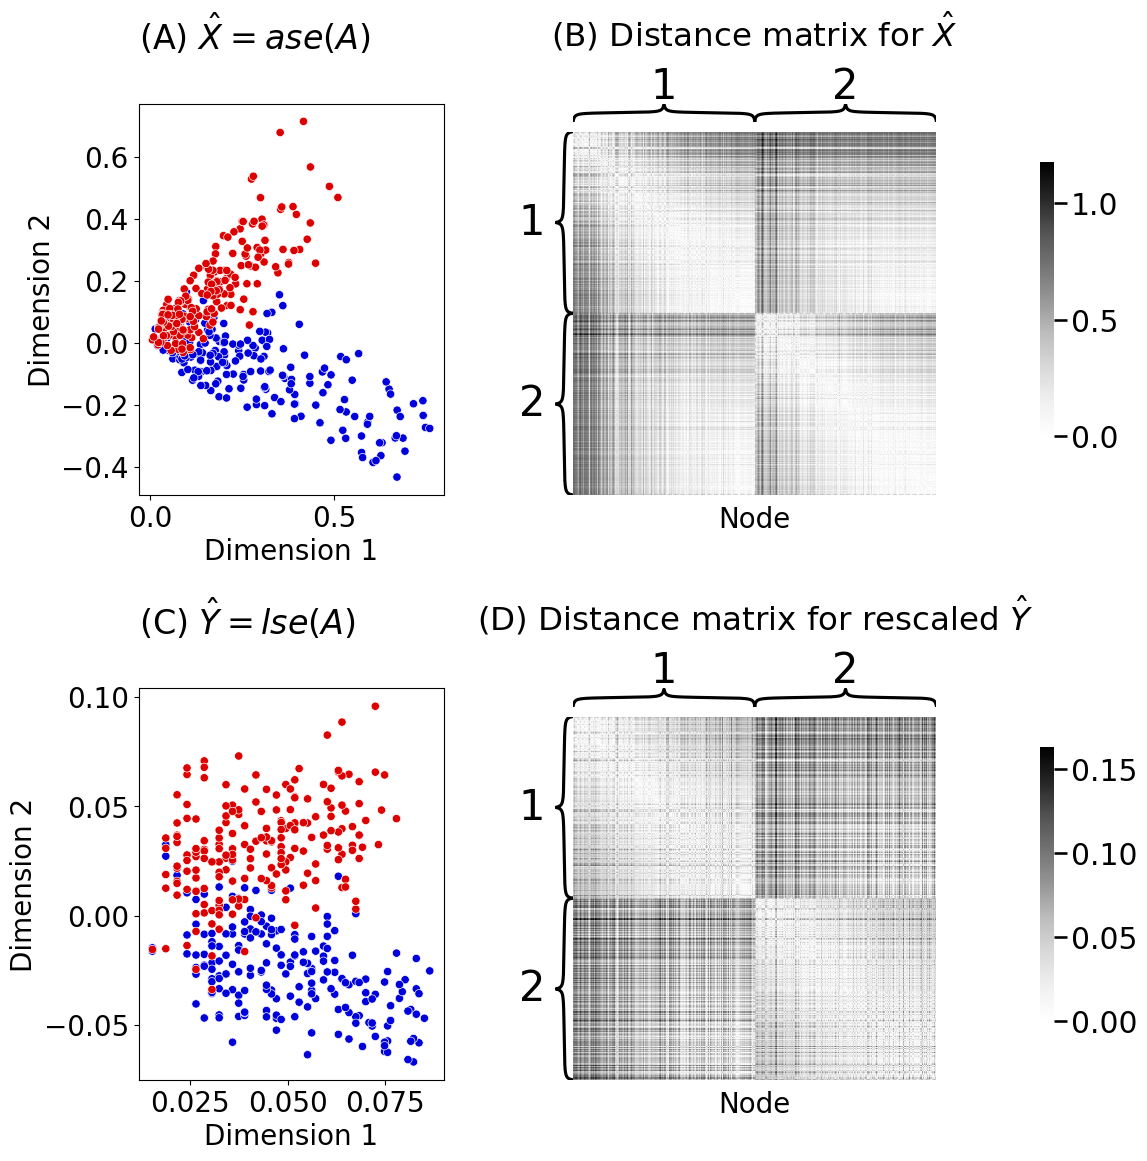
\includegraphics[width=\linewidth]{representations/ch6/Images/dcsbm_lse.png}
    \caption[LSE vs ASE, heavy-tailed example]{\textbf{(A)} the estimated latent positions, \textbf{(B)} the pairwise distances of estimated latent positions, \textbf{(C)} the estimated latent positions from \texttt{lse}, \textbf{(D)} the pairwise distances of the estimated latent positions from \texttt{lse}.}
    \label{fig:ch6:lse:dcsbm_lse}
\end{figure}

\subsection{Why do we use \texttt{lse}?}

The reasons to use \texttt{lse} are very similar to the reasons to use \texttt{ase}, which we explored in Section \ref{sec:ch6:ase:whyuse}. 

\subsubsection{When do we use \texttt{lse} over \texttt{ase}, and vice-versa?}

The primary difference between \texttt{lse} and \texttt{ase} is illustrated by example in Figure \ref{fig:ch6:lse:dcsbm_lse}. \texttt{ase} will capture estimates of latent positions, whereas \texttt{lse} will capture estimates of latent positions of the population network laplacian. Loosely, this has the consequence that \texttt{lse} will produce ``scaled'' estimates of latent positions that have been adjusted for degree differences in the underlying network. 

Often, we will want to learn about latent structures that are not related to the degrees of the nodes in the network. In such cases, these scaled estimates produced by \texttt{lse} will often make latent structure that we might want to find more obvious both visually (in heatmaps and pairs plots) and algorithmically (through the use of downstream models to identify latent structure from your estimated latent positions). 

A primary visualization to determine whether \texttt{ase} or \texttt{lse} are appropriate is to look at the {node degree histogram}. The node degree histogram is a histogram of the degrees for each node in the network. We can do this by first computing the node degrees in the network, and then plotting them as a histogram, using the insights that we build in Section \ref{sec:ch4:prop-net:degree}. Let's investigate this for the $DCSBM_n(\vec z, \vec \theta, B)$ sample we generated above:

\begin{lstlisting}[style=python]
import seaborn as sns
import pandas as pd

# compute the degrees for each node, using the
# row-sums of the network
degrees = A.sum(axis = 0)

# plot the degree histogram

df = pd.DataFrame({"Node degree" : degrees, "Community": z})
sns.histplot(data=df, x="Node degree", bins=20, color="black", hue="Community")
\end{lstlisting}

The key feature that we look for is whether the degree histogram is \textit{right-skewed} or \textit{heavy tailed}. Remember from Section \ref{sec:ch4:regularization:logscale} that a distribution is right-skewed if it ``tails off'' towards the relatively large values in the positive direction. In these situations, the node degrees are lower-bounded by zero (the networks are simple, so all the adjacencies $a_{ij}$ are either $0$ or $1$, and the node degrees are sums of adjacencies), so this is generally just referred to as a ``heavy tailed degree distribution'', since it can only ``tail off'' to the right (since it is bounded to the left by $0$). Note that in Figure \ref{fig:ch6:lse:degree}(A), the degree distribution for nodes across both communities tails off to the right. For $DCSBM_n(\vec z, \vec \theta, B)$ random networks where the degree-correction factors $\theta_i$ tend to have mostly relatively small values, but some relatively large values, that the degree is lower-bounded by $0$ will tend to yield heavy tailed degree distributions. 

This contrasts from $SBM_n(\vec z, B)$ random networks and $DCSBM_n(\vec z, \vec \theta, B)$ random networks where the degree-correction factor $\theta_i$ is constant for all nodes in the same community, which will tend to have symmetric degree distributions for each community.

\begin{lstlisting}[style=python]
Asbm = sbm([nk, nk], B)

# row-sums of the network
degrees_sbm = Asbm.sum(axis = 0)
\end{lstlisting}

The histogram for an $SBM_n(\vec z, B)$ random network is shown in Figure \ref{fig:ch6:lse:degree}(B). Note that the degree histogram appears to have two ``peaks'', and neither peak is particularly heavy tailed (they both look fairly mirrored). This plot provides evidence that the degree-distribution is not heavy tailed.

\begin{figure}[h]
    \centering
    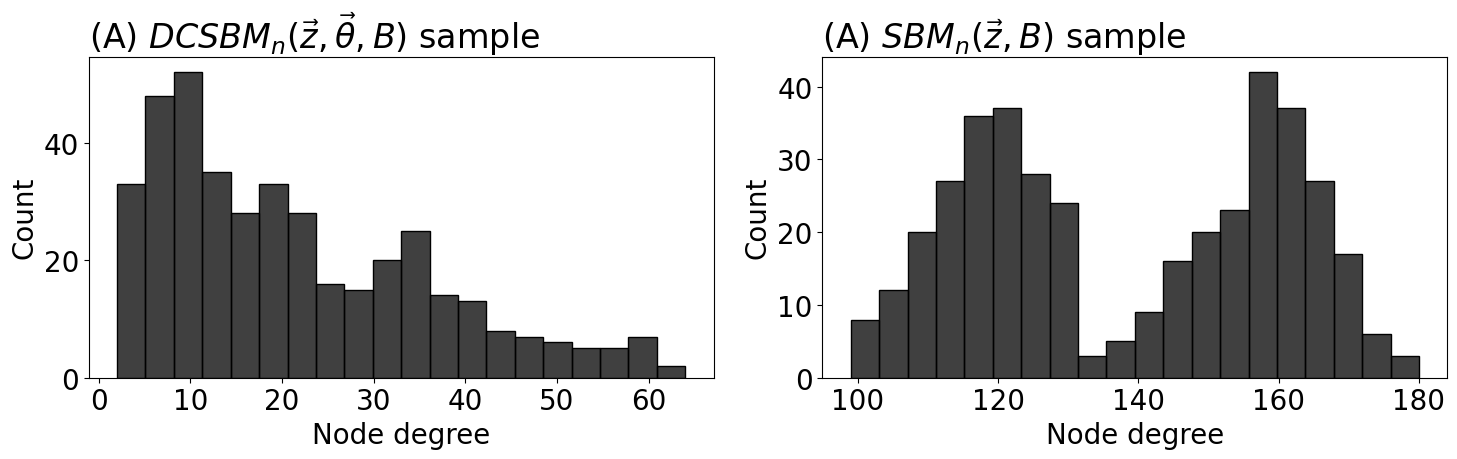
\includegraphics[width=\linewidth]{representations/ch6/Images/lse_degree.png}
    \caption[degree histogram for $DCSBM_n(\vec z, \vec \theta, B)$]{\textbf{(A)} the degree histogram for a $DCSBM_n(\vec z, \vec \theta, B)$ network, where the degree-correction factors are not equal for the nodes in the network. \textbf{(B)}the degree histogram for a $SBM_n(\vec z, B)$ network.}
    \label{fig:ch6:lse:degree}
\end{figure}

Heavy-tailed degree distributions frequently arise in real data \cite{Qin2013Sep, Muldoon2016Feb, Prakash2010}. This pattern is particularly apparent in networks that share features of core-periphery networks from Section \ref{sec:ch5:psd_block}, where a selection of nodes (the \textit{core}) have much higher node degrees than the nodes outside of the core (the \textit{periphery}) \cite{Prakash2010}. This pattern can materialize concurrently with other patterns, such as the example that we saw above with a $DCSBM_n(\vec z, \vec \theta, B)$ network with heterogeneous $\theta_i$s and homophilic networks. 

When you can identify a heavy-tailed degree distribution from visualizations such as the node degree histogram, \texttt{lse} may be advantageous to use over \texttt{ase}. This might assist you in uncovering latent structure in the estimates of latent positions that you use downstream in your analysis.

\begin{comment}
\section{Expected values and random networks}

\subsection{Expected values and the adjacency matrix}
Back in Section \ref{sec:ch4:prop-net:degree}, you learned about the degree matrix. To obtain the degree matrix, we started by computing the node degrees, where:
\begin{align*}
    d_i = \sum_{j = 1}^n a_{ij}
\end{align*}

Once we computed the node degrees, the degree matrix was the diagonal matrix where:
\begin{align*}
    D &= \begin{bmatrix}
        d_1 & & \\
        & \ddots & \\
        & & d_n
    \end{bmatrix},
\end{align*}

To understand the expected node degree, it is important to first clarify the expected outcome at a particular edge. We'll do this with as little statistics knowledge as possible. If $\mathbf x$ is a random quantity that takes one of two possible outcomes ($0$ or $1$), then the expected value is:
\begin{align*}
    \mathbb E[\mathbf x] = 1 Pr (\mathbf x = 1) + 0 Pr(\mathbf x = 0),
\end{align*}
where $Pr(\mathbf x = k)$ is just the probability that the random quantity $\mathbf x$ takes the value $k$. This is a very simple case of a statistical result that is commonly known as the \textit{Law of the Unconscious Statistician} (LoTUS).

We have already seen an instance of a random quantity that takes one of two possible outcomes ($0$ or $1$) in our work: the adjacencies for a random network, $\mathbf a_{ij}$. Remember that for an adjacency $\mathbf a_{ij}$, that $\mathbf a_{ij}$ behaves like flipping a coin which lands on Heads (a value of $1$) with probability $p_{ij}$, or Tails (a value of $0$) with probability $1 - p_{ij}$. Therefore, the expected value of each adjacency $\mathbf a_{ij}$ is:
\begin{align*}
    \mathbb E[\mathbf a_{ij}] &= p_{ij}
\end{align*}

This logic extends directly to matrices. If $\mathbf X$ is a matrix, then its expected value is:
\begin{align*}
    \mathbb E[\mathbf X] &= \begin{bmatrix}
        \mathbb E[\mathbf x_{11}] & \hdots & \mathbb E[\mathbf x_{1n}] \\
        \vdots & \ddots & \vdots \\
        \mathbb E[\mathbf x_{n1}] & \hdots & \mathbb E[\mathbf x_{nn}]
    \end{bmatrix}
\end{align*}
So, the expected value of a matrix is the matrix of expected values of each entry.

This has an important implication for our purposes. If $\mathbf A$ is an $IER_n(P)$ random network, then:
\begin{align*}
    \mathbb E[\mathbf A] = P
\end{align*}

Now, for our purposes, this is a little bit obtuse: we see samples $A$, not the random network $\mathbf A$, in practice.

As it turns out, there is another result that can help us here. If $\mathbf x$ and $\mathbf y$ are two finite random variables (which they always will be, in our case), then the expectation of the sum is the sum of the expectations. In words, we can write this down as:
\begin{align*}
    \mathbb E[\mathbf x + \mathbf y] = \mathbb E[\mathbf x] + \mathbb E[\mathbf y].
\end{align*}

Let's extend this to the case of taking an sum. Remember that a sum of $M$ numbers $x^{(m)}$ is defined as:
\begin{align*}
    \sum_{m = 1}^M x^{(m)}
\end{align*}
If we instead had $M$ random numbers $\mathbf x^{(m)}$, when we compute the expected value of the sum, it is the sum of the expected values:
\begin{align*}
   \mathbb E\left[\sum_{m = 1}^M x^{(m)}\right] &= \sum_{m = 1}^M \mathbb E\left[\mathbf x^{(m)}\right]
\end{align*}

So, let's imagine that we have $M$ adjacency matrices $\mathbf A^{(m)}$ that are each independent $IER_n(P)$ random networks with the same probability matrix. The expected average adjacency matrix would be:
\begin{align*}
    \mathbb E\left[\frac{1}{M}\sum_{m = 1}^M \mathbf A^{(m)}\right] &= 
\end{align*}
\end{comment}




\newpage
\section{Multiple network representation learning}
\label{sec:ch6:multinet}

In this section, we're going to learn a number of strategies that are useful from when we have multiple networks. When we have multiple networks, there are a variety of questions that we might want to ask. In this section, we'll focus on a few of these questions, and provide structured ways to learn representations of these networks that allow us to address our downstream questions. We'd recommend that you glance back at the $COSIE_{n, M}\left(V, \{R_m\}_{m = 1}^M\right)$ random networks in Section \ref{sec:ch5:multi}, as these will be critical for understanding many of the techniques that we cover in this section.

We'll use a running example of brain networks, which we describe in Remark \ref{box:ch6:multinet:ex}.

\begin{floatingbox}[h]\caption{Alien and human brain networks}
\label{box:ch6:multinet:ex}
Let's imagine that you're a brain network, and you've been given the unique task of learning about a group of $4$ human-like alien life forms that were recently discovered. When studying their brains (in a non-invasive way), you make the remarkable discovery that aliens and humans have brain areas that do similar things across species. These $n=100$ brain areas will be the nodes of your network.

For both aliens and humans, there are two hemispheres (communities) in the brain. However, you make a somewhat startling discovery in that while human brains tend to have a homophilic structure (with more connections between nodes in the same hemisphere of the brain), alien brains tend to have a disassortative structure (with more connections between nodes in the opposite hemisphere of the brain).

For this reason, you want to be able to obtain suitable representations of your networks that you can use downstream to learn about the differences between human and alien brain networks.
\end{floatingbox}

Let's generate our working examples:

\begin{lstlisting}[style=python]
from graspologic.simulations import sbm
import numpy as np

n = 100  # the number of nodes
M = 8  # the total number of networks
# human brains have homophilic block structure
Bhum = np.array([[0.2, 0.02], [0.02, 0.2]])
# alien brains have a disassortative block structure
Balien = np.array([[0.02, 0.2], [0.2, 0.02]])

# generate 4 human and alien brain networks
A_humans = [sbm([n // 2, n // 2], Bhum) for i in range(M // 2)]
A_aliens = [sbm([n // 2, n // 2], Balien) for i in range(M // 2)]
# concatenate list of human and alien networks
As = A_humans + A_aliens

# 1 = left hemisphere, 2 = right hemisphere for node communities
zs = [1 for i in range(n // 2)] + [2 for i in range(n // 2)]
labels = ["L" for i in range(n // 2)] + ["R" for i in range(n // 2)]
\end{lstlisting}

The collection \texttt{As} is a list of adjacency matrices, where the first $4$ entries correspond to the human brains, and the second $4$ entries correspond to the alien brains. \texttt{zs} corresponds to community labels for the nodes of the networks, where \texttt{1} is a place-holder for ``Left hemisphere'', and \texttt{2} is a placeholder for ``Right hemisphere''. We also added a second list of community labels, \texttt{labels}, which correspond to the true names. You might find having dummy place-holders for discrete community labels (such as \texttt{zs}) to be handy when you want to do things like run one-hot encodings, and you might find having more informative node labels (such as \texttt{labels}) handy for when you want to visualize, plot, and learn from your networks.

\begin{figure}[h]
    \centering
    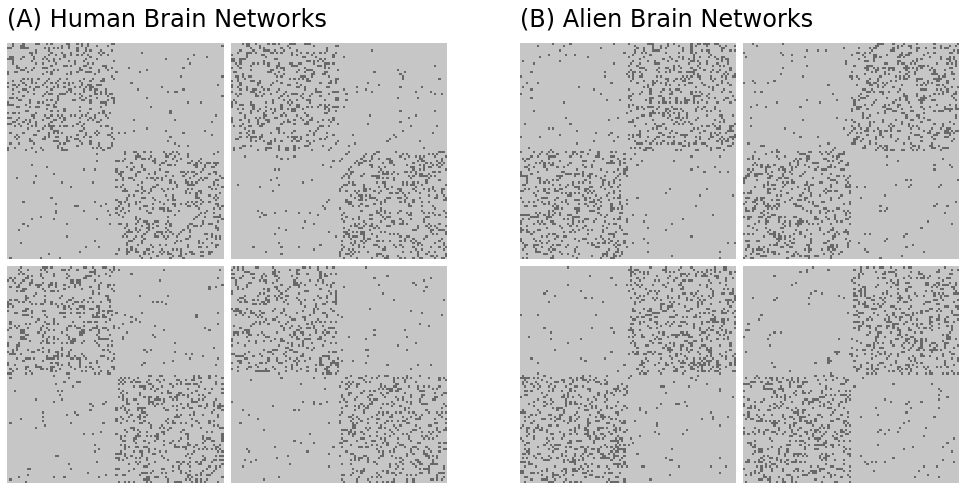
\includegraphics[width=\linewidth]{representations/ch6/Images/multi_ex.png}
    \caption[Alien/Human brain network example]{\textbf{(A)} the human brain networks, and \textbf{(B)} the alien brain networks.}
    \label{fig:ch6:multinet:ex}
\end{figure}
The human and alien brain networks are plotted (nodes are ordered by the node hemisphere, the ``community'') in Figure \ref{fig:ch6:multinet:ex}. Notice that whereas the human brain networks tend to have more connections within the same hemisphere (the on-diagonal blocks), the alien brain networks tend to have more connections between the two hemispheres (the off-diagonal blocks). 

Remember, our goal is to identify whether humans and aliens have similar or different structure to their nodes. We're going to try to to embed our brain networks into some lower-dimensional space. Once the nodes are in a lower dimensional space, we can use standard downstream techniques to learn latent structure from the network.

\subsection{Embedding networks through averaging}

The first place that we might start is to average our networks together, and then embed the result with spectral embedding. It turns out that, if we can safely assume that all of the networks in a collection are similar, in the sense that there is no particular reason that one network should be distinct from another, this is actually the right case. Formally, analyzing embeddings of the average tends to be appropriate when the networks have the same distribution.

As we'll see, based on what we know already, using a naive average and embedding the result is fairly inappropriate for the data. Let's see what happens when we average the networks:

\begin{lstlisting}[style=python]
# compute the global average across all networks
global_mean_network = np.array(networks).mean(axis=0)
\end{lstlisting}

\begin{figure}[h]
    \centering
    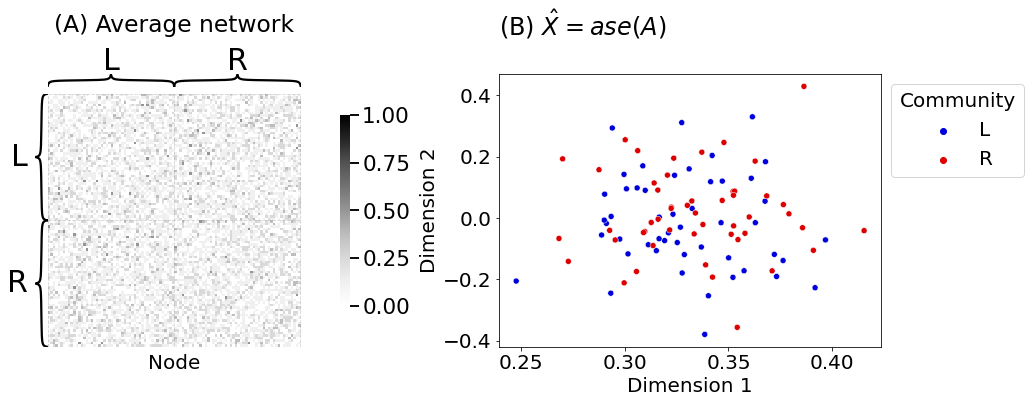
\includegraphics[width=\linewidth]{representations/ch6/Images/multinet_avg.png}
    \caption[Average embedding]{\textbf{(A)} the average network produced by averaging the adjacency matrices for humans and aliens together, \textbf{(B)} the latent positions of the average networks.}
    \label{fig:ch6:multinet:avg}
\end{figure}

We visualize this network as a heatmap in Figure \ref{fig:ch6:multinet:avg}(A). Not that the salient topological structures that we identified in Figure \ref{fig:ch6:multinet:ex} have been decimated, in the sense that they are not visually prominent anymore. This is because our analysis of Figure \ref{fig:ch6:multinet:ex} suggested that the networks had a different underlying block matrix (humans appeared to have a ``homophilic'' structure, and aliens appeared to have a ``dissassortative'' structure). The degree of decimation of structure (visually) is a function of the specific network samples you obtain, as well as the disparity between the underlying random networks.

Next, we embed the result using \texttt{ase}, with a target dimensionality of $2$ since the networks have two communities:

\begin{lstlisting}[style=python]
from graspologic.embed import AdjacencySpectralEmbed as ase
Xhat = ase(n_components=2).fit_transform(global_mean_network)
\end{lstlisting}

We plot the resulting latent position estimates in Figure \ref{fig:ch6:multinet:avg}(B). One thing that should jump out immediately is that, as we might have expected, this approach has severe drawbacks. The decimation of latent structure (visually, in the heatmap) was further reflected in the decimation of structure in the downstream spectral embeddings.

\subsubsection{Conditional averaging and then embedding}

From our initial visualizations in Figure \ref{fig:ch6:multinet:ex}, it might have been easy to predict why the averaging procedure might fail: the networks from our visualizations in \ref{fig:ch6:multinet:ex} had prominent ``opposing'' structures, in that all of the humans showed a homophilic structure, but all of the aliens showed a disassortative structure. As we explored above, when we took a naive average and embedded the result, we decimated structure between the two hemispheres. For this reason, a more principled approach that we might think up would be to average only networks that appear somewhat homogeneous (in terms of the underlying probability matrices).

In this case, we could visually look at the network heatmaps in Figure \ref{fig:ch6:multinet:avg} and immediately conclude that all of the human networks might have a similar block matrix, and all of the alien networks might also have a similar block matrix. Since the probability matrices for $SBM_n(\vec z, B)$ random networks are a function of the community assignments of nodes $\vec z$ (which is the same across the groups of networks) and the block matrix $B$, as we learned in Section \ref{sec:ch5:ier:sbm_pmtx}, we might be able to visually conclude that the human networks are somewhat homogeneous and the alien networks are somewhat homogeneous.

Therefore, it might feel appropriate to \textit{conditionally average}, where we compute averages looking only within a particular group. In this situation, that would entail computing an average adjacency matrix for the human networks, an average adjacency matrix for the alien networks, and then embedding each separately. 

Let's see how this works out for us:

\begin{lstlisting}[style=python]
hum_mean = np.array(A_humans).mean(axis=0)
alien_mean = np.array(A_aliens).mean(axis=0)
\end{lstlisting}
\begin{figure}[h]
    \centering
    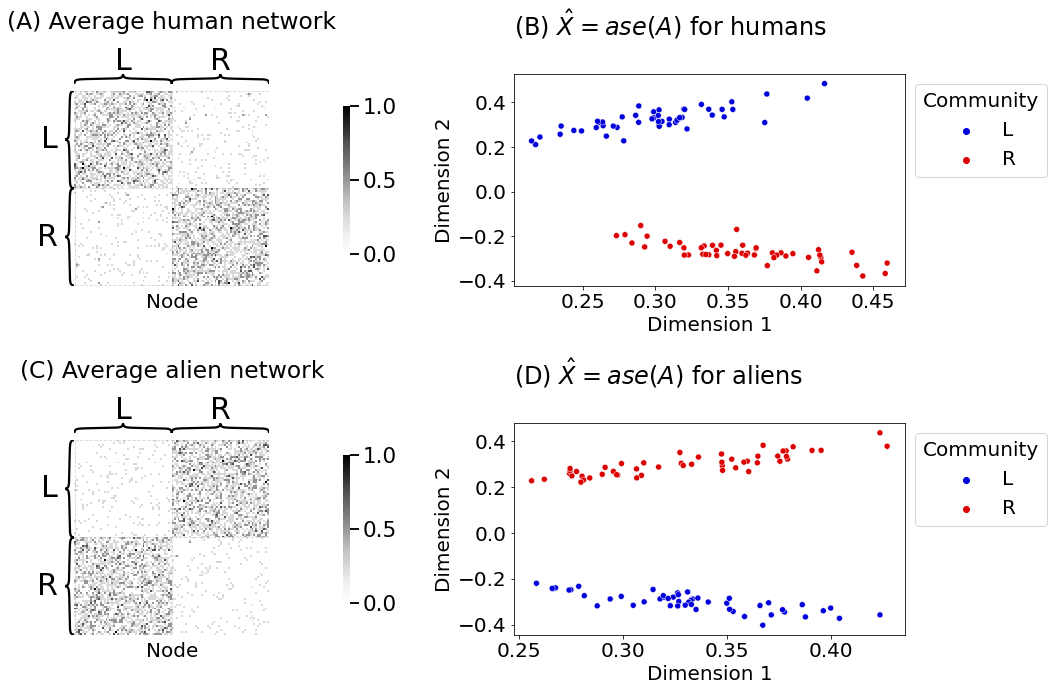
\includegraphics[width=\linewidth]{representations/ch6/Images/cond_avg.png}
    \caption[conditional average embeddings]{\textbf{(A)} the average human adjacency matrix, \textbf{(B)} the spectral embedding of the average human adjacency matrix, \textbf{(C)} the average alien adjacency matrix, \textbf{(D)} the spectral embedding of the average alien adjacency matrix.}
    \label{fig:ch6:multinet:cond_avg}
\end{figure}
We plot the conditional averages in Figure \ref{fig:ch6:multinet:cond_avg}(A) and \ref{fig:ch6:multinet:cond_avg}(C). Note that averaging conditionally has not decimated our known structure to the adjacency matrices.

Next, we embed the conditional averages, again using \texttt{ase}:

\begin{lstlisting}[style=python]
Xhat_hum = ase(n_components=2).fit_transform(hum_mean)
Xhat_alien = ase(n_components=2).fit_transform(alien_mean)
\end{lstlisting}

The latent position estimates for the conditional averages is shown in Figure \ref{fig:ch6:multinet:cond_avg}(B) and \ref{fig:ch6:multinet:cond_avg}(D). When we look at the latent position estimates, it appears that community structure has been preserved, which means that we have not decimated the latent structure that we want to investigate further downstream. This is good news for us, however we have another problem. A reasonable way we might want to approach determining whether human and alien brain networks differ would be to compare the latent position estimates, right? Unfortunately, this is not that easy to do, due to the problem we mentioned in Section \ref{sec:ch6:spectral:nonidentifiable}, the non-identifiability problem. Particularly, the estimates that we produced for humans and aliens, \texttt{Xhat\_hum} and \texttt{Xhat\_alien}, might not be rotated in the same orientation. 

\subsubsection{What other problems does taking averages suffer from?}

There are a variety of reasons why averaging, even when we conditionally average human and alien brain networks separately, are unideal. When we average the network unconditionally, we can decimate latent structure, like we learned right above. Even when we average the networks conditionally, if all human brain networks and all alien brain networks come from the same distribution, we still encounter problems. The networks end up, potentially disasterously, not being properly oriented in comparable latent spaces, due to the non-identifiability problem. This means that while we could learn (with conditional averaging) about the humans and alien brain networks separately, we could not learn about them together. Our analysis would be restricted to each group of networks individually.

Finally, and potentially most catastrophically, is the big assumption that we made to average the networks conditionally: that all human brain networks, or separately all alien brain networks, come from the same distribution. This assumption, when viewed through a statistical lens, makes little sense: individual to individual, or more generally network to network, it seems rather unreasonable to believe that numerous samples would come from exactly same distribution. In fact, in many cases where it would be desirable to analyze multiple networks, this is the {opposite} of the reason we might analyze multiple networks in the first place. 

Additionally, in light of the concern that we first brought up in Section \ref{sec:ch5:sbm:modularity}, the shared structure (or disparate structure) that exists between our networks might not be immediately obvious to we. If the human and alien brain networks were simply had their nodes not pre-arranged in community order, that humans had a homophilic structure and aliens had a disassortative structure would not have been visually perceptible. 

While we might anticipate there is shared structure between groups of networks that are in the same categories, more often than not, it's going to make sense to choose techniques that are not limited in their level of reasonability to cases where the assumptions of shared structure are imposed (e.g., by averaging). This holds true with the example we gave back in multiple network modelling in \Section \ref{sec:ch5:multi} (where we discussed social networks from Facebook, Twitter, and Linkedin), it holds true in many cases where you look at brain networks like here, and it's going to make sense in many other domains.

In any case where we have reason to believe that each network comes from a unique distribution, we are going to want a way to reflect that in our algorithm. Let's see how we might approach the problem with these limitations of averaging in mind. 

\subsection{Different types of multiple network representation learning}

Let's take a moment to explore some of the possible general approaches we could take in multiple-network representation learning. At some point we need to combine the many individual representations of our networks into one, and there are at least three possible places where we could do this: combining the networks together, combining the networks separately, and combining the embeddings. Each of these eventually results in a latent position representation for our networks. It's important to note that in all of these approaches, we are simply learning representations for our groups of networks. 

All types of multiple-network representation learning strategies that we describe in this section entail first constructing a joint matrix. A \textit{joint matrix} is a matrix which is derived from multiple networks, and summarizes them in such a way that it facilitates downstream analysis. The specific way that the joint matrix is determined from the data depends on the specific multiple-netework representation learning technique.

\subsubsection{Combining the networks together}

With this approach, we start with a set of networks, and then the joint matrix will represent the adjacency matrix of a new network (that summarizes information about all of the other networks that went into it). We then embed and analyze the joint matrix and its embedding directly. What we did before, averaging the human and alien networks, was an example of combining our networks -- we  averaged all of our adjacency matrices, and then we embedded the result. 

This tends to be effective when you want to study a property which is common across all of the networks, and you believe network-to-network differences that do not relate to the property of interest to be effectively noise. Unfortunately, it suffers from many of the issues we just mentioned. This approach is summarized in Figure \ref{fig:ch6:multinet:comb}.

\begin{figure}[h]
    \centering
    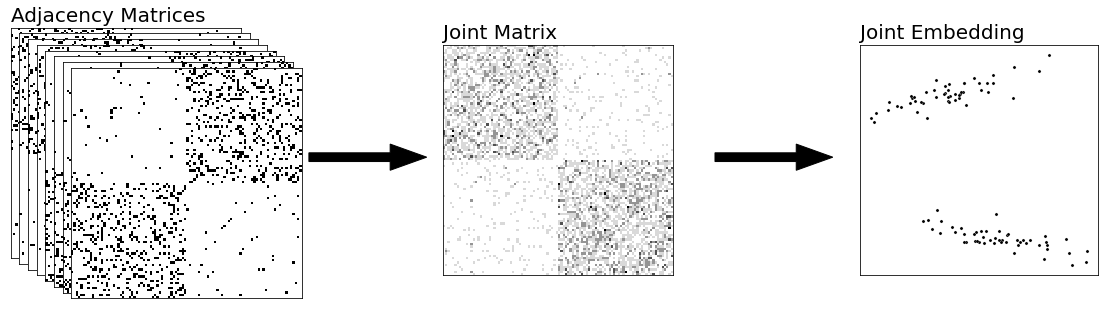
\includegraphics[width=\linewidth]{representations/ch6/Images/joint_comb.png}
    \caption[Combining networks together]{The process of combining your networks to acquire a joint matrix, and then embedding the result to obtain a multiple network representation.}
    \label{fig:ch6:multinet:comb}
\end{figure}

\subsubsection{Combining the embeddings}

The next approach to multiple-network representation learning that we will learn about is combining the embeddings themselves into the joint matrix. With this approach, we first obtain representations from each network, either with adjacency spectral embedding or with some other single-network representation learning strategy. Next, these embeddings are combined into a joint matrix, and then we learn from this joint matrix using sequential approaches (such as additional embeddings of the joint matrix). Multiple adjacency spectral embedding (\texttt{mase}), which we will learn about soon, is an example of this approach. This approach is summarized in Figure \ref{fig:ch6:multinet:comb_emb}.

\begin{figure}[h]
    \centering
    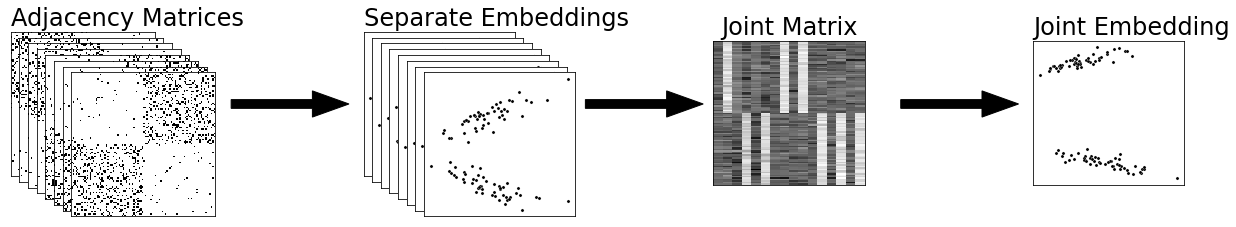
\includegraphics[width=\linewidth]{representations/ch6/Images/comb_emb.png}
    \caption[Combining embeddings together]{The process of embedding your networks to obtain separate representations, combining these individual representations to obtain a joint matrix, and then obtaining a representation of the joint matrix to obtain a multiple network represenatation.}
    \label{fig:ch6:multinet:comb_emb}
\end{figure}


\subsubsection{Combining networks separately}

The above approach is effective when our networks have shared structure, where the final embedding describes shared structures across the nodes of the networks, and we obtain other descriptive features about the joint embedding that describe particularities about the individual networks as they relate to this shared structure. The joint embedding that we obtain tends to summarize information across the nodes, as we will learn soon. 

However, there are situations in which we might want to keep our embeddings separate, with the exception of wanting them to co-exist in a related latent space, meaning the embeddings aren't rotations of each other. This addresses the problem that we noticed in Section \ref{sec:ch6:spectral:nonidentifiable}. When we approach multiple-network representation learning in this manner, we can directly compare the embeddings of the separate networks. An example of combining the networks separately is the Omnibus embedding (OMNI), and is illustrated in Figure \ref{fig:ch6:multinet:comb_sep}.

\begin{figure}[h]
    \centering
    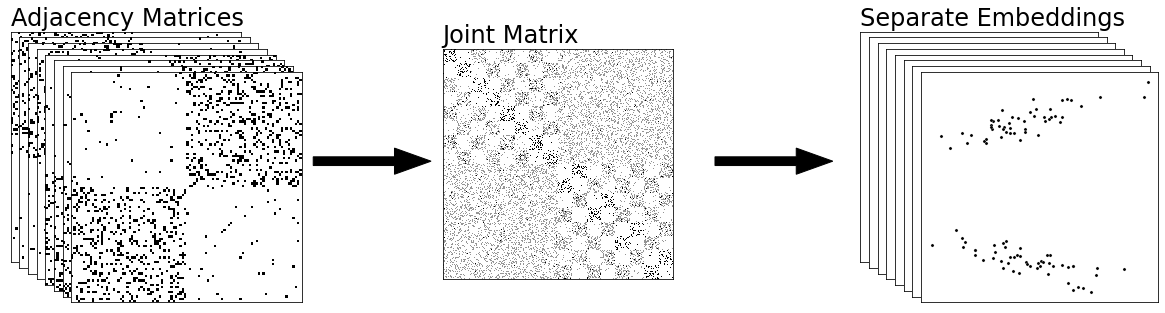
\includegraphics[width=\linewidth]{representations/ch6/Images/comb_sep.png}
    \caption[Combining networks separately]{The process of combining your networks to acquire a joint matrix, and then embedding the result to obtain a multiple network representation.}
    \label{fig:ch6:multinet:comb_sep}
\end{figure}

For the rest of this section, we'll explore the strengths and weaknesses of different techniques which use these latter two approaches. 


\subsection{Multiple Adjacency Spectral Embedding}

Multiple Adjacency Spectral Embedding, or \texttt{mase} is a technique which combines embeddings by concatennating and re-embedding the separate latent positions into a single space. The advantage of \texttt{mase} is we don't actually need each network to be generated from the same distribution - we only need the nodes of the different networks to be aligned and have similar ``meaning'' across the networks. What this means is that node $1$ in network $1$ has the same literal interpretation as node $1$ in networks $2$ through $M$, and so on for all $n$ nodes of the network. In your brain network, for instance, node one is the first region, node two is the second region, ... and this property applies to all of the nodes in the network and across all networks in your collection.

\texttt{mase} is probably the easiest to understand if you know how adjacency spectral embeddings work. We have some number of networks, and (like we said above) their nodes are aligned. The goal of \texttt{mase} is to embed the networks into a shared space with shared latent dimensions. 

\texttt{mase} is based on the common subspace independent-edge (COSIE) model that you learned about in Section \ref{sec:ch5:multi:cosie}. If you recall, with the COSIE model, you learned that across your networks, there might be some underlying homogeneity: in your brain networks, for instance, there might be communities that are shared across all of the networks. Simultaneously, these networks are distinct for one reason or another in terms of the underlying probability matrix: for instance, a pair of humans might have different probabilities for particular edges being connected or disconnected, or a pair of individuals one of whom is human and the other is alien might have different patterns to their probability matrices all together. In this sense, the COSIE model allowed you to capture both the homogeneity and heterogeneity across different networks simultaneously.

Let's go back to your group of human and alien brains and try using \texttt{mase} to embed them rather than averaging. Then, we will dive deeper into what goes on under the hood. 

\begin{lstlisting}[style=python]
from graspologic.embed import MultipleASE as mase

# Use mase to embed everything
mase = mase(n_components=2)
# fit_transform on the human and alien networks simultaneously
# + combines the two lists
latents_mase = mase.fit_transform(networks)
\end{lstlisting}

\subsubsection{How does \texttt{mase} work?}

\paragraph*{Embedding your networks}

The first step in the \texttt{mase} algorithm is to spectrally embed each network. This step is discussed in the preceding sections for \texttt{ase} in Section \ref{sec:ch6:ase} and \texttt{lse} in Section \ref{sec:ch6:lse}. 

When you know ahead of time how many dimensions that you want, you would perform your ASE with the desired number of dimensions here. It is a good rule of thumb to over-embed than it is to under-embed dimensionality wise; that is, if we embed into too many dimensions, we might have more challenges downstream when we try to learn from the networks, but if we embed into too few dimensions, we risk discarding latent structure (and will therefore have no hope of finding it downstream). In general for this first step of \texttt{mase}, a good number of embedding dimensions tends to be $\log_2(n)$. When $n$ is $100$ as in your example, this comes to about $7$:

\begin{lstlisting}[style=python]
from graspologic.embed import AdjacencySpectralEmbed as ase

dhat = int(np.ceil(np.log2(n)))
# spectrally embed each network into ceil(log2(n)) dimensions with ASE
joint_matrix = [ase(n_components=dhat).fit_transform(network) for network in As]
\end{lstlisting}

We plot the spectral embeddings of a human and an alien (showing only the first two dimensions) in Figure \ref{fig:ch6:multinet:mase:ase}. Notice that the separate embeddings individually preserve the community structure across both humans and aliens. Figure \ref{fig:ch6:multinet:mase:ase_joint}(A) shows the embeddings across all networks as heatmaps.

\begin{figure}[h]
    \centering
    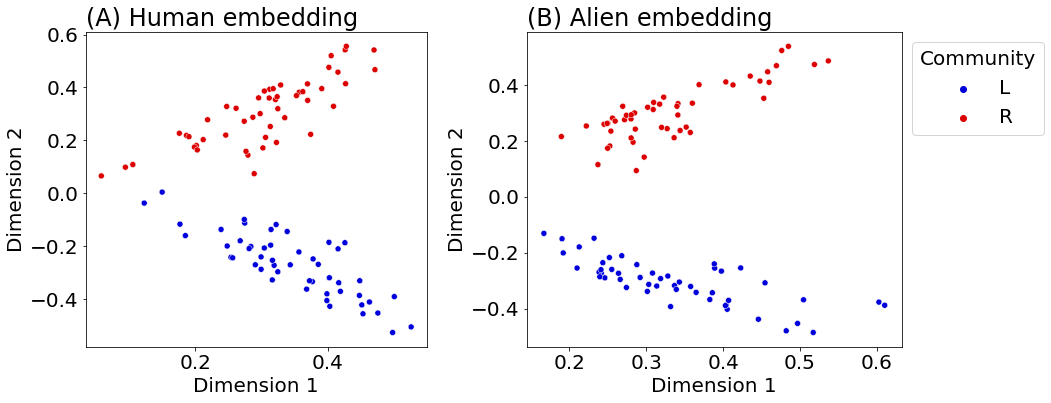
\includegraphics[width=0.8\linewidth]{representations/ch6/Images/mase_ase.png}
    \caption[\texttt{mase} \texttt{ase} step]{\textbf{(A)} the spectral embedding for a human network, and \textbf{(B)} the spectral embedding for an alien network.}
    \label{fig:ch6:multinet:mase:ase}
\end{figure}

It is important to note that these embeddings do not live in the same latent space just yet; that is, they may be oriented differently, and the embeddings are not directly comparable.

\paragraph*{Calculating a shared latent space}

Now comes the interesting part. Our goal is to find some way to take each of these individual embeddings and combine them. We want to find a reasonable way of doing this.

To do this, what we'll effectively do is take each of our individual network embeddings, and concatenate them horizontally. Because the rows of these matrices are all aligned - meaning, row 1 corresponds to node 1 for all four matrices - you can actually think of each node as having (in this case) $Md$ latent dimensions: there are $d$ latent dimensions for each of your $M$ networks. In this case, since $\hat d = 7$ and $M = 8$, this means that each node has $7 \times 8 = 56$ latent dimensions associated with it ($7$ per network).

You don't actually need separate matrices to express this idea: the natural thing to do would be to just concatenate all of the matrices horizontally into a single $n \times Md$ matrix, where $n$ is the number of nodes (the rows of the resulting matrix), and $Md$ is the number of latent dimensions associated with each node (the columns of the resulting matrix). This matrix is called the joint matrix, since it is a composition of information from the $M$ total networks. We can concatenate the adjacency matrices to construct the joint matrix using numpy:

\begin{lstlisting}[style=python]
# Concatenate your embeddings horizontally into a single n x Md matrix
joint_matrix = np.hstack(joint_matrix)
\end{lstlisting}

This matrix is plotted in Figure \ref{fig:ch6:multinet:mase:ase_joint}(B), and is known as the \textit{joint matrix} for \texttt{mase}.

\begin{figure}[h]
    \centering
    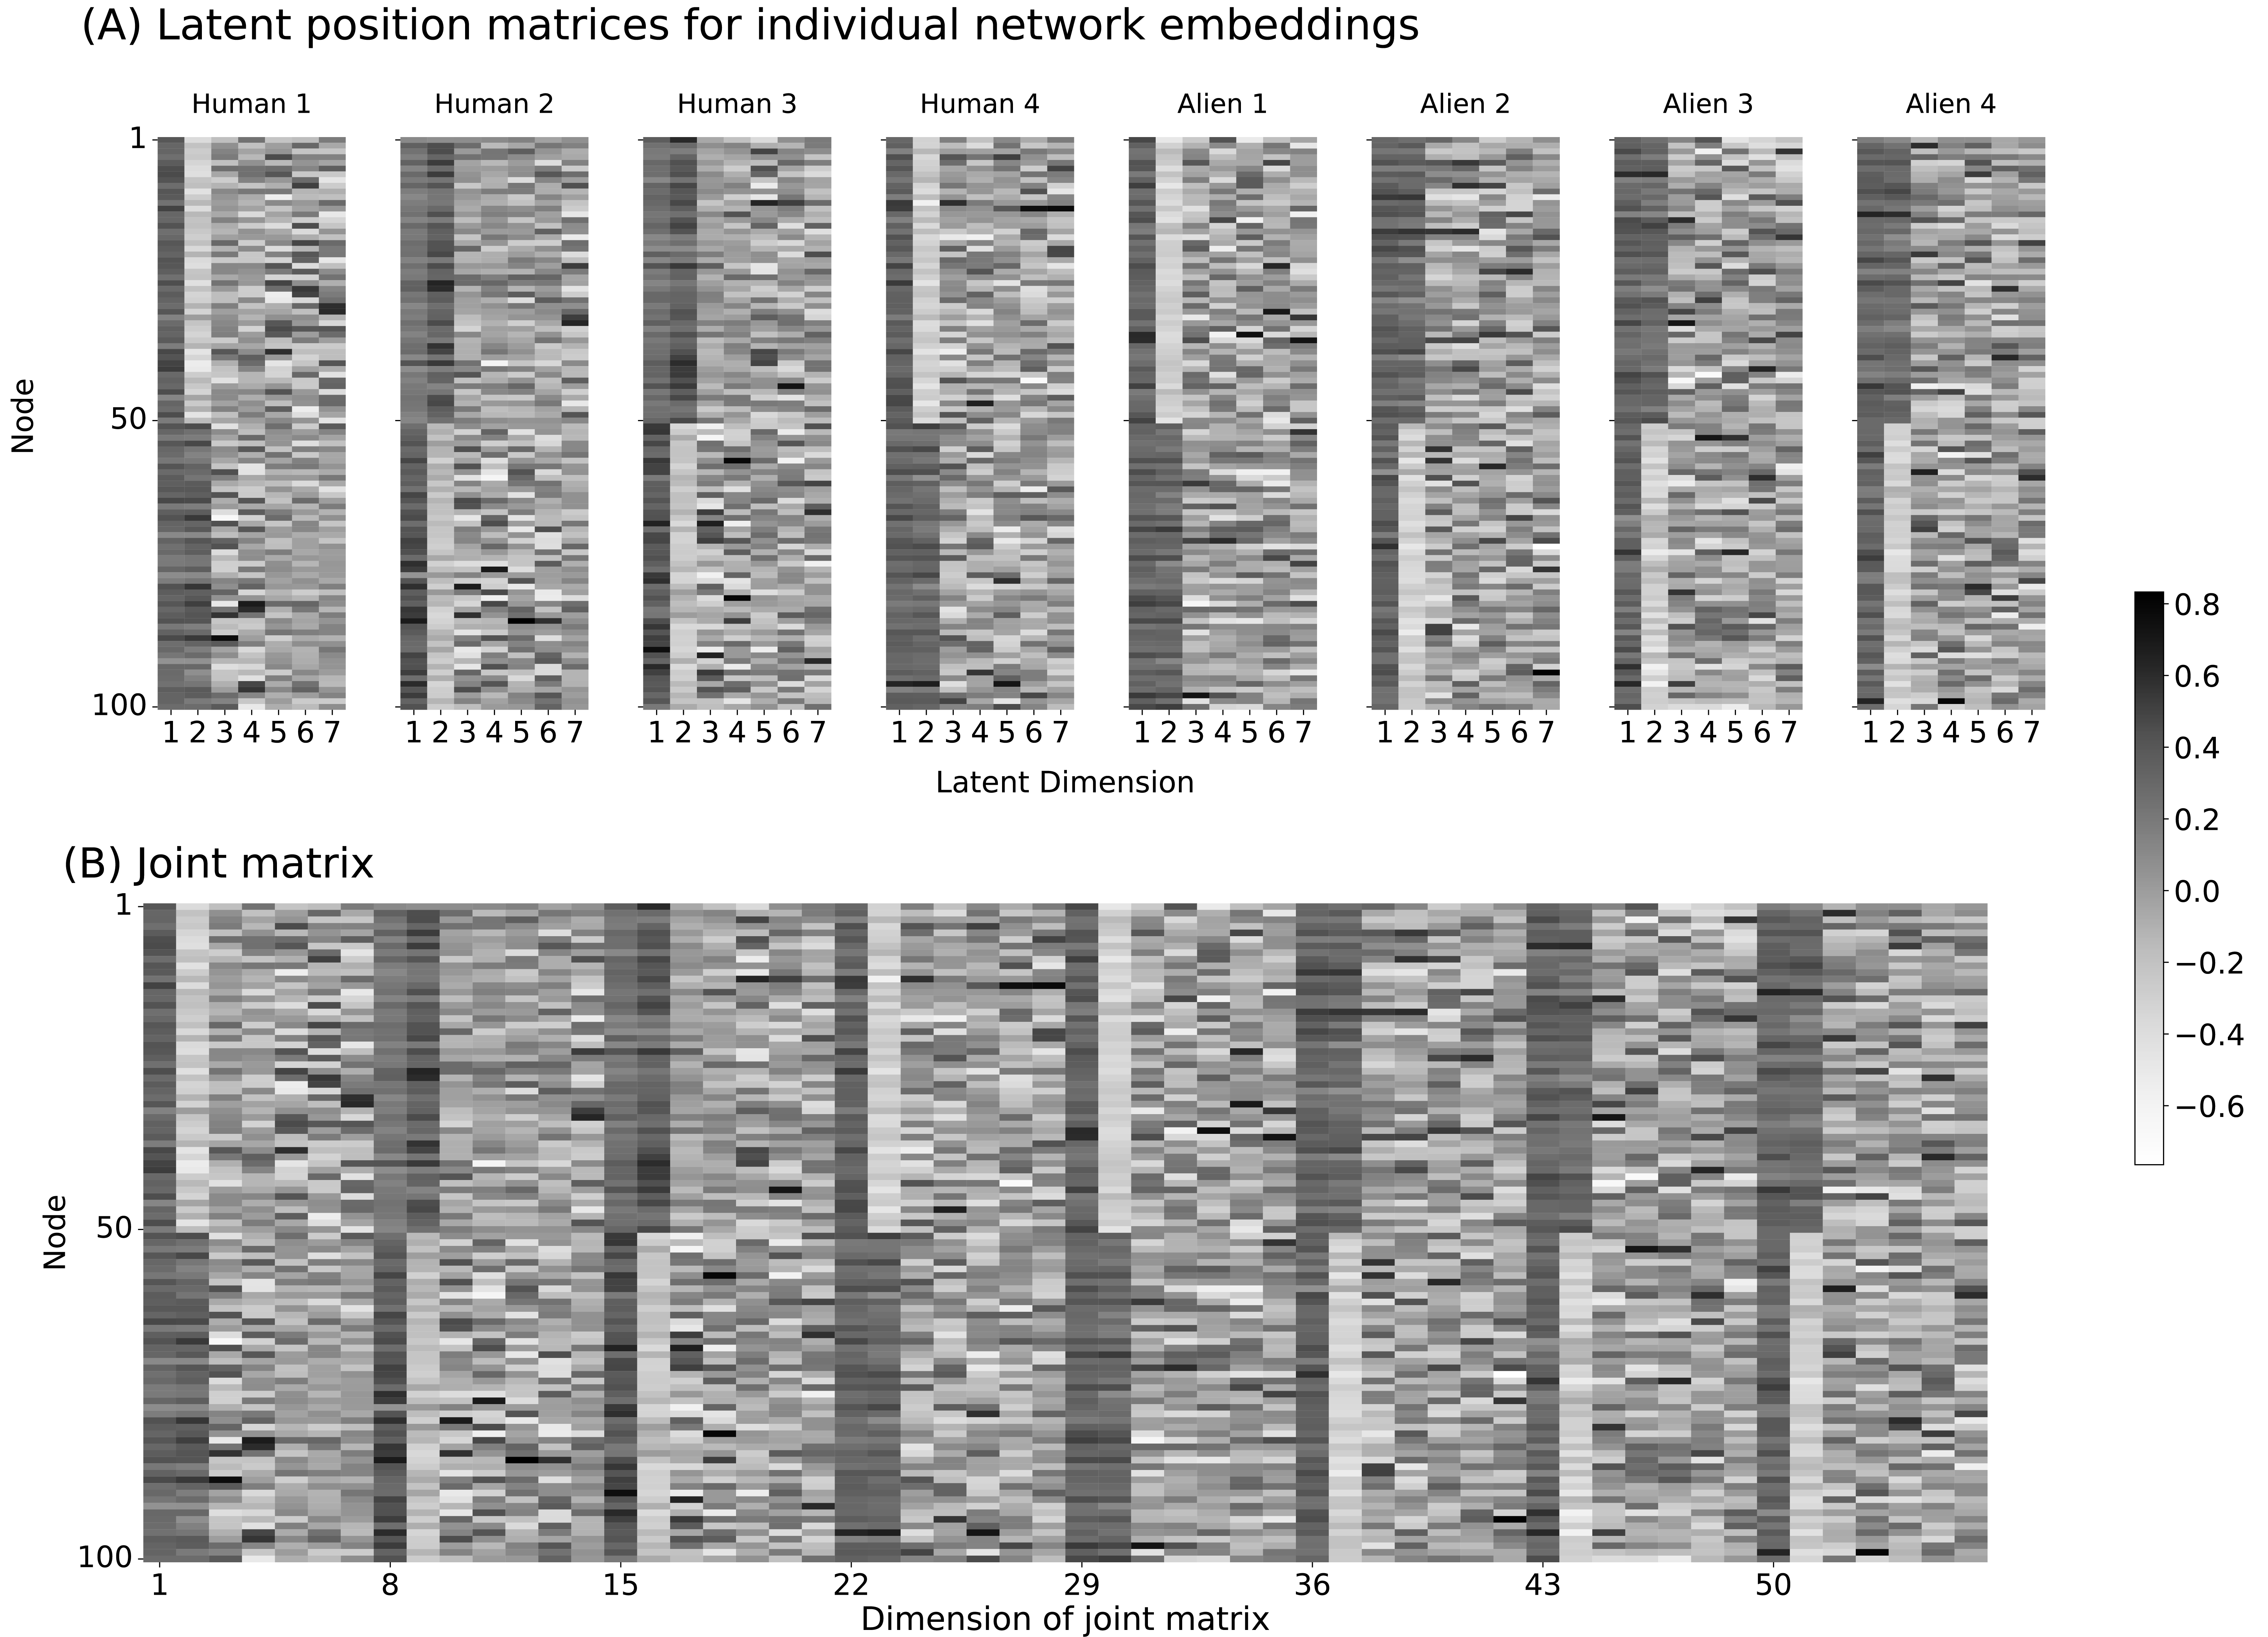
\includegraphics[width=\linewidth]{representations/ch6/Images/mase_embed_joint.png}
    \caption[\texttt{mase} joint matrix]{\textbf{(A)} the separate embeddings for each network. \textbf{(B)} the joint matrix, which concatenates the separate embeddings for each network (horizontally).}
    \label{fig:ch6:multinet:mase:ase_joint}
\end{figure}

When we look at the joint matrix oriented in this manner, we can see the property that we are going to exploit in our next step. Notice that there looks to be a lot of redundant information in this matrix. In particular, the first column always appears to be relatively constant across all of the networks. The second column of every embedding looks like it tends to separate the first $50$ nodes (which were the left hemisphere) from the next $50$ nodes (which were the right hemisphere). Successive dimensions tend to look like noise.

This sort of redundancy of some of the qualitative features of the columns is, in fact, exploitable. This is despite the fact that the columns aren't exactly identical in their behavior (for instance, for some of the networks, the second embedding dimension has high values for the first 50 nodes and low values for the second 50 nodes, or low values for the first 50 nodes and high values for the second 50 nodes). The important idea is that there is some notion of similar information being conveyed that we can use to simplify this problem even further.

\paragraph{Embedding the joint matrix to create a joint embedding}

So now we have a joint matrix, but you have a new issue to address: there's a lot of redundant information which is common to many of these embeddings (such as the second dimension tending to separate the left from the right), and some information common only to a subset of these embeddings (such as that some of the networks have the second dimension having high values for the first group of nodes and low values for the second group of nodes, and vice versa for the other networks). The way in which this redundancy is conveyed is not consistent from embedding to embedding, nor even within network groupings (the patterns in some of the human and alien network embeddings are different, even though the underlying $SBM_n(\vec z, B)$ random networks are homogeneous for networks in the same group), which is an instance of the rotational non-identifiability from Section \ref{sec:ch6:spectral:nonidentifiable} problem.

Fortunately, spectral embedding is an ideal candidate for picking out these sorts of ``redundancies'' that arise across columns of our matrix. Spectral embedding allows us to capture the redundancy of the qualitative aspects of these columns, and obtain the general idea of what they each convey numerically. For this, we will use \texttt{pca}, or Principle Components Analysis. The process is nearly identical to what we did before for \texttt{ase} in Algorithm \ref{alg:ch6:ase}, in that we perform an \texttt{svd}, and retain the top $d$ left singular vectors. This is called an \textit{unscaled spectral embedding}, because we are not weighting the left singular vectors by the square roots of the singular values (like we did in \texttt{ase}).

Through this process, what you are effectively doing is now embedding your joint matrix, to obtain a joint embedding. Let's see how this works. Since the networks have two communities, we'll use $2$ embedding dimensions:

\begin{lstlisting}[style=python]
def unscaled_embed(X, d):
    U, s, Vt = np.linalg.svd(X)
    return U[:,0:d]

Vhat = unscaled_embed(joint_mtx, 2)
\end{lstlisting}

The result of this unscaled embedding is known as an \textit{estimate of the shared latent positions}, and is denoted by the matrix $\hat V$. $\hat V$ has $n$ rows and $d$ columns, so each row $\hat{\vec v}_i$ is an estimate of the shared latent position of node $i$. 

We plot the estimate of the shared latent positions $\hat V$ in Figure \ref{fig:ch6:multinet:mase:shared_lpm}. Note that the estimated shared latent positions convey the shared structure between human and alien brains: the left and right hemispheres are appreciably different. 

\begin{figure}[h]
    \centering
    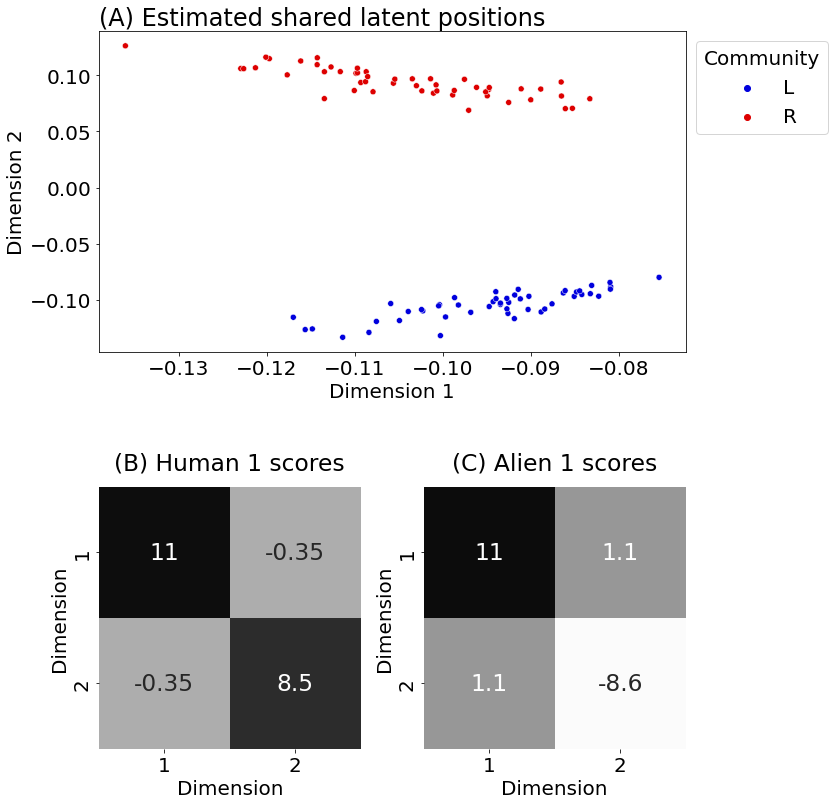
\includegraphics[width=\linewidth]{representations/ch6/Images/mase_shared_lpm.png}
    \caption[parameter estimates from \texttt{mase}]{\textbf{(A)} The estimated shared latent positions of the human and alien brains. \textbf{(B)} the estimated scores for the first human network, \textbf{(C)} the estimated scores for the first alien network.}
    \label{fig:ch6:multinet:mase:shared_lpm}
\end{figure}

\subsubsection{Building representations for each network}

Exactly how is the joint embedding we created related to all of our separate, original networks? Remember that under the COSIE model in Section \ref{sec:ch5:multi:cosie}, the probability matrix for the $i^{th}$ network could be described as:

\begin{align*}
    P^{(i)} &= VR^{(i)}V^\top \numberthis \label{eqn:ch6:mase:e1}
\end{align*}

where $V$ conveyed the homogeneity across all $M$ networks (the \textit{shared latent positions}), and $R^{(i)}$ conveyed the unique aspects of the probability matrix for a particular network $i$ (the unique \textit{score matrices}).

Next, remember that in the COSIE model, an assumption was that $V$ was orthonormal. For an orthonormal matrix $V$ with $n$ rows and $n$ columns, $V^\top V = VV^\top = I_n$. This means that conceptually that by pre-multiplying by $V^\top$ and post-multiplying by $V$ in Equation \eqref{eqn:ch6:mase:e1}:
\begin{align*}
    V^\top P^{(i)}V &= V^\top VR^{(i)} V^\top V \\
    \Rightarrow R^{(i)}&= V^\top P^{(i)} V,\numberthis \label{eqn:ch6:mase:score_est}
\end{align*}
which is because $V$ was orthonormal.

In practice, however, we have two problems.

\paragraph*{Estimates of the shared latent positions are not orthonormal}

We do not have the shared latent positions, we have an estimate of the shared latent positions $\hat V$. $\hat V$ is the first $d$ columns of the left singular vectors $U$ of the joint matrix. While the full left singular vector matrix is orthonormal (by definition of the \texttt{svd}, in Remark \ref{box:ch6:svd_results}), it is generally favorable to \textit{reduce} the dimensionality when we embed, below the number of nodes in the network so that we can learn from the shared latent position matrix later. Unfortunately, this disrupts the orthonormality, and $\hat V$ is no longer orthonormal when we discard the last $n - d$ columns.

\paragraph*{We do not observe the probability matrix}

Remember that a hurdle that we experienced in the \texttt{ase} was that we could obtain a perfect estimate of the latent position matrix (up to a rotation) if we knew the probability matrix. However, we do not have a probability matrix, because the probability matrix was a merely an intuitive construct that we use to conceptualize our network sample, and to evaluate the techniques that we developed if our conceptual model is correct. 

In its place, we simply used the adjacency matrix. The reason that we settled on the approach that we settled on for \texttt{ase} was that the eigendecomposition procedure in Algorithm \ref{alg:ch6:evd} would not work unless the matrix was positive semi-definite, but we had no such restriction with the \texttt{ase} procedure in Algorithm \ref{alg:ch6:ase} that used the \texttt{svd}. Likewise, no part of our procedure for \texttt{mase} is restrictive of positive semi-definiteness to obtain a real answer.

\paragraph*{Ignorance proves blissful (again)}

While these limitations might feel impactful, just like with the \texttt{ase}, we can ignore them (for the time being). Using Equation \eqref{eqn:ch6:mase:score_est} for the score matrices, we simply plug in the estimate of the shared latent positions for $V$, and the adjacency matrix $A^{(i)}$ for the probability matrix, to obtain an estimate of the score matrix:

\begin{align*}
    \hat R^{(i)} &= \hat V^\top A^{(i)}\hat V.
\end{align*}

Let's see how to do this in practice with our networks:

\begin{lstlisting}[style=python]
# stack the networks into a numpy array
As_ar = np.asarray(As)
# compute the scores
scores = Vhat.T @ As_ar @ Vhat
\end{lstlisting}
We plot the estimated score matrices in Figure \ref{fig:ch6:multinet:mase:shared_lpm}(B) and (C) for a human and alien network, respectively. Notice in particular that the human networks and the alien networks leverage different combinations of the two latent dimensions to ``reconstruct'' the score matrix, much like in Section \ref{sec:ch5:multi:cosie:score} when the Facebook/Twitter and Linkedin networks used different score matrices to convey the disparate structure in the networks. In particular, the second estimated shared latent dimension, which is the shared latent dimension that conveys the disparity between the left and right communities, is much different for the human and alien networks. This highlights that the human and alien networks convey the disparate community structure (humans having a homophilic structure, aliens a dissassortative structure) through the latent dimension which distinguishes the communities.

Finally, we use this with the COSIE model in Equation \eqref{eqn:ch6:mase:e1} to obtain that:
\begin{align*}
    \hat P^{(i)} &= \hat V \hat R^{(i)} \hat V^\top.
\end{align*}
Let's see how this works out in practice, by computing the true probability matrix for the humans and aliens, and comparing it to the estimated probability matrix for the humans and aliens. We compute the true probability matrix using the results from Section \ref{sec:ch5:ier:sbm_pmtx}.

\begin{lstlisting}[style=python]
from graphbook_code import generate_sbm_pmtx

Phum = generate_sbm_pmtx(zs, Bhum)
Palien = generate_sbm_pmtx(zs, Balien)
Pests = Vhat @ scores @ Vhat.T
\end{lstlisting}

The true probability matrices for humans and aliens are shown in Figure \ref{fig:ch6:multinet:mase:est_prob}(A) and (C), and are compared to the estimated probability matrices for aliens and humans are shown in Figure \ref{fig:ch6:multinet:mase:est_prob}(B) and (D). Note that \texttt{mase} is able to recover both the homophilic structure of the human brain networks and the disassoratative structure of the alien brain networks across estimated shared latent dimension 2 in Figure \ref{fig:ch6:multinet:mase:shared_lpm}(A), which separated the left and right communities. 

\begin{figure}[h]
    \centering
    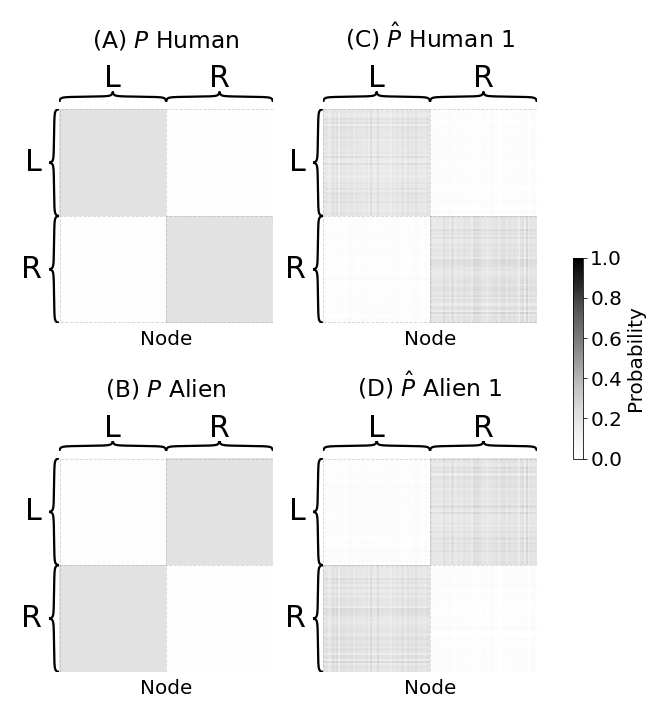
\includegraphics[width=0.8\linewidth]{representations/ch6/Images/mase_probs.png}
    \caption[probability matrix estimates for \texttt{mase}]{\textbf{(A)} the probability matrix for human networks, \textbf{(B)} the estimated probability matrix for the first human network. \textbf{(C)} the probability matrix for alien networks, \textbf{(D)} the estimated probability matrix for the first alien network.}
    \label{fig:ch6:multinet:mase:est_prob}
\end{figure}

\subsubsection{Using \texttt{mase} in practice}

The \texttt{mase} algorithm is shown in Algorithm \ref{alg:ch6:mase}. 

\begin{algorithm}[h]\caption{Multiple adjacency spectral embedding (\texttt{mase})}
\label{alg:ch6:mase}
\KwData{$A^{(1)}, ..., A^{(M)}$ a collection of $M$ networks with $n$ nodes.\newline $d$ the desired latent dimensionality.}
\KwResult{the estimated shared latent position matrix and the estimated score matrices.}
\SetAlgoLined

For each $A^{(i)}$, obtain $\hat X^{(i)} = \texttt{ase}\left(A^{(i)}, \log_2(n)\right)$, for $i = 1, \hdots, M$, via Algorithm \ref{alg:ch6:ase}. 

Let $J = \begin{bmatrix}\hat X^{(1)} & \hdots & \hat X^{(M)}\end{bmatrix}$ be the joint matrix, consisting of a column-wise concatenation of the individual estimated latent position matrices.

Let $U, \Sigma, V = \texttt{svd}(J)$.

Let $\hat V = U_d$, the first $d$ columns of the left singular vectors of $J$. 

Let $\hat R^{(i)} = \hat V^\top A^{(i)}\hat V$, for $i = 1, \hdots, M$.

\Return{$\hat V, R^{(1)}, \hdots, R^{(M)}$}
\end{algorithm}

You can run the \texttt{mase} algorithm using \texttt{graspologic}, which streamlines the procedure that we outlined above:

\begin{lstlisting}[style=python]
from graspologic.embed import MultipleASE as mase

d = 2
mase_embedder = mase(n_components=d)
# obtain an estimate of the shared latent positions
Vhat = mase_embedder.fit_transform(As)
# obtain an estimate of the scores
Rhat_hum1 = mase_embedder.scores_[0]
# obtain an estimate of the probability matrix for the first human
Phat_hum1 = Vhat @ mase_embedder.scores_[0] @ Vhat.T
\end{lstlisting}

\subsection{Omnibus Embedding}
\label{sec:ch6:multinet:omni}

The \textit{Omnibus Embedding} (\texttt{omni}) embeds networks separately while keeping them all into the same latent space (that is, they will be properly rotated to align with one another). What this means is that the embeddings for each network after the omnibus embedding can be compared. \texttt{omni} does not attempt to separately identify shared and unique structures across networks, unlike \texttt{mase} (which considered shared structures via the estimated shared latent positions and unique structure through the separate estimated score matrices for each network).

\subsubsection{How does \texttt{omni} work?}

\paragraph*{Computing the omnibus matrix}

The first step in \texttt{omni} is to compute the omnibus matrix, which is the joint matrix used by \texttt{omni}. The \textit{omnibus matrix} for a collection of $M$ networks with $n$ nodes is the $Mn \times Mn$ matrix $O$, where for each $n \times n$ block $O^{(i, j)}$, it is:
\begin{align*}
    O^{(i, j)} &= \frac{1}{2}\left(A^{(i)} + A^{(j)}\right).
\end{align*}
The resulting $(i, j)$ block of the omnibus matrix is itself a $n \times n$ matrix, and the Omnibus matrix looks like this:
\begin{align*}
    O &= \begin{bmatrix}
        O^{(1, 1)} & \hdots & O^{(1, M)} \\
        \vdots & \ddots & \vdots \\
        O^{(M, 1)} & \hdots & O^{(M, M)}
    \end{bmatrix} = \begin{bmatrix}
        A^{(1, 1)} & \hdots & \frac{1}{2}\left(A^{(1)} + A^{(M)}\right) \\
        \vdots & \ddots & \vdots \\
        \frac{1}{2}\left(A^{(1)} + A^{(M)}\right) & \hdots &  A^{(M)}
    \end{bmatrix}.
\end{align*}
By construction, notice that the Omnibus matrix is symmetric with respect to the blocks themselves, in that $O^{(i, j)} = O^{(j, i)}$. However, if these individual blocks are not themselves symmetric, the omnibus matrix might not be symmetric. Since the blocks of the omnibus matrix are combinations of adjacency matrices, and adjacency matrices are symmetric when the underlying networks are undirected, the omnibus matrix is symmetric when the collection of networks are undirected. 

Let's consider only the first two networks (human networks), and construct a simple omnibus matrix from these. We can do this with \texttt{numpy}:

\begin{lstlisting}[style=python]
omni_ex = np.block([[As[0], (As[0]+As[1])/2],
                 [(As[1]+As[0])/2, As[1]]])
\end{lstlisting}

We visualize this small omnibus matrix in Figure \ref{fig:ch6:multinet:omni:ex}. We illustrate the first two networks in \ref{fig:ch6:multinet:omni:ex}(A) and \ref{fig:ch6:multinet:omni:ex}(B), and the resulting omnibus matrix of the first two networks in \ref{fig:ch6:multinet:omni:ex}(C).

\begin{figure}[h]
    \centering
    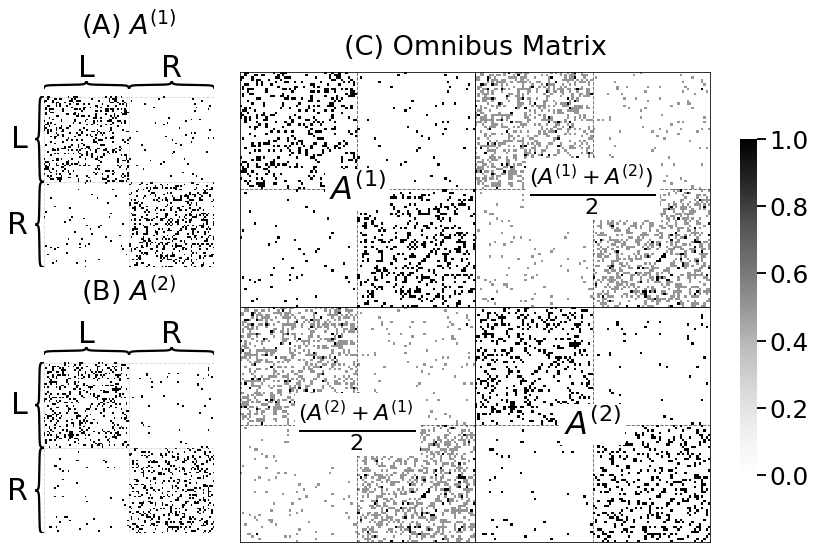
\includegraphics[width=\linewidth]{representations/ch6/Images/omni_ex.png}
    \caption[simple example of omnibus matrix]{\textbf{(A)} the first human network, \textbf{(B)} the second human network. \textbf{(C)} the omnibus matrix of the first two human networks.}
    \label{fig:ch6:multinet:omni:ex}
\end{figure}

We can use \texttt{graspologic} to obtain the omnibus matrix for our collection of networks:
\begin{lstlisting}[style=python]
from graspologic.embed.omni import _get_omni_matrix
omni_mtx = _get_omni_matrix(As)
\end{lstlisting}

The full omnibus matrix for all $8$ networks is shown in Figure \ref{fig:ch6:multinet:omni:fullmtx}(A). You can conceptualize the omnibus matrix as the adjacency matrix of a new network from your collection of networks, where the nodes from each network form a single node in the new network. A subnetwork induced on the omnibus matrix by the nodes from a single network is the original network itself (the on-diagonal blocks of the omnibus matrix $O^{(i,i)}$). The subnetwork formed by the nodes of a network $i$ and the nodes of another network $j$ provides information about how similar (or different) the networks $i$ and $j$ are (the off-diagonal blocks of the omnibus matrix $O^{(i, j)}$). This incorporation of information about each network in relation to the other networks is what will allow \texttt{omni} to properly orient the latent positions across your collection of networks.

\paragraph*{Embedding the omnibus matrix}

The next step to \texttt{omni} is to embed the omnibus matrix using \texttt{ase}. This creates an estimate of the latent position matrix for the omnibus matrix itself. When you embed the $Mn \times Mn$ omnibus matrix into $d$ dimensions, you obtain an estimated latent position matrix that has $Mn \times d$ dimensions. A good rule of thumb for the omnibus embedding is to use $\log_2(n)$ embedding dimensions.

\begin{figure}[h]
    \centering
    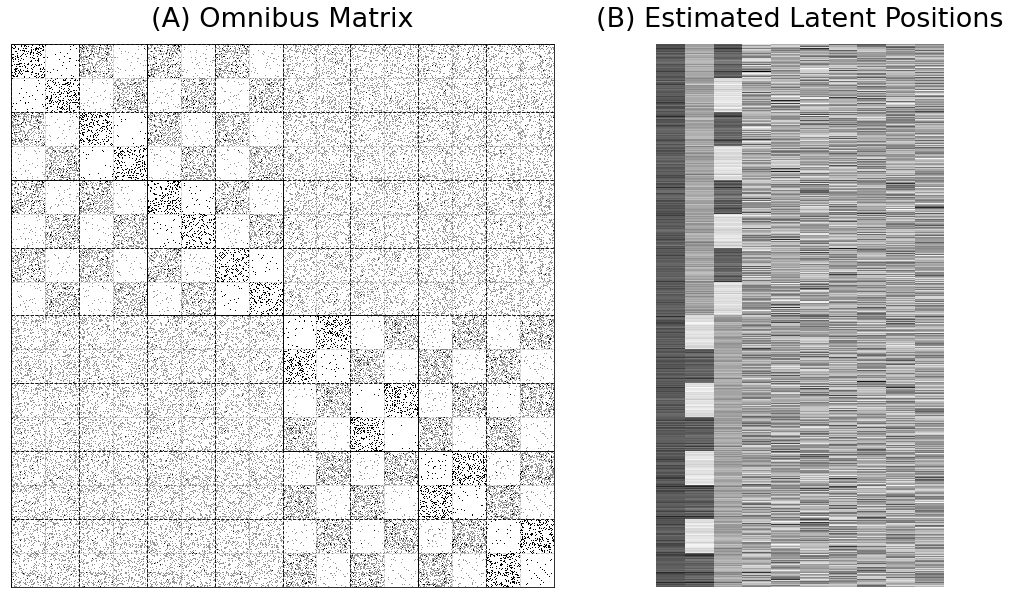
\includegraphics[width=\linewidth]{representations/ch6/Images/omni_mtx.png}
    \caption[omnibus matrix and omnibus embedding]{\textbf{(A)} the omnibus matrix, and \textbf{(B)} the embedded omnibus matrix.}
    \label{fig:ch6:multinet:omni:fullmtx}
\end{figure}

\begin{lstlisting}[style=python]
from graspologic.embed import AdjacencySpectralEmbed as ase

dhat = int(np.ceil(np.log2(n)))
Xhat_omni = ase(n_components=dhat).fit_transform(omni_mtx)
\end{lstlisting}

The estimated latent positions for the omnibus matrix are shown in Figure \ref{fig:ch6:multinet:omni:fullmtx}.

\paragraph*{Extracting oriented estimated latent positions}

The last step of \texttt{omni} is to obtain the properly oriented latent position estimates for each network. Remember that the omnibus matrix effectively could be conceptualized as the adjacency matrix for a new network, where the $Mn$ nodes of this new network are the $n$ nodes of each of the original $M$ networks. Visually, the $Mn \times d$ estimated latent position matrix looks like this:
\begin{align*}
    \hat X &= \begin{bmatrix}
        \hat X^{(1)} \\
        \hat X^{(2)} \\
        \vdots \\
        \hat X^{(M)}
    \end{bmatrix},
\end{align*}
where each set of estimated latent positions $\hat X^{(i)}$ which are $n \times d$ matrices correspond to the estimated latent positions for the network $A^{(i)}$.

To obtain the latent positions for each network explicitly, you can reshape the $Mn \times d$ matrix into an $m \times n \times d$ tensor, and look at the individual slices of the tensor corresponding to the estimated latent position matrix for each network. You can do this with \texttt{numpy} like this:

\begin{lstlisting}[style=python]
M = len(networks)
n = len(networks[0])

# obtain a M x n x d tensor
Xhat_tensor = Xhat_omni.reshape(M, n, -1)
# the estimated latent positions for the first network
Xhat_hum1 = Xhat_tensor[0,:,:]
\end{lstlisting}

The estimated latent positions for each network are illustrated in Figure \ref{fig:ch6:multinet:omni:individual} for all of the networks in our collection. The second and third dimensions capture most of the signal disparity between the human and alien networks, so we show scatter plots for these two dimensions. Note that the human networks appear to have the nodes in the same relative positions, and the alien networks appear to have the nodes in the same relative positions, which is a function of the rotational alignment created by \texttt{omni}. Had we embedded the networks separately, this would not have been the case. On the other hand, note that the human brain network nodes and the alien brain network nodes appear to have different patterns in the embeddings, which is a function of the unique disparities between human and alien brain networks.

\begin{figure}[h]
    \centering
    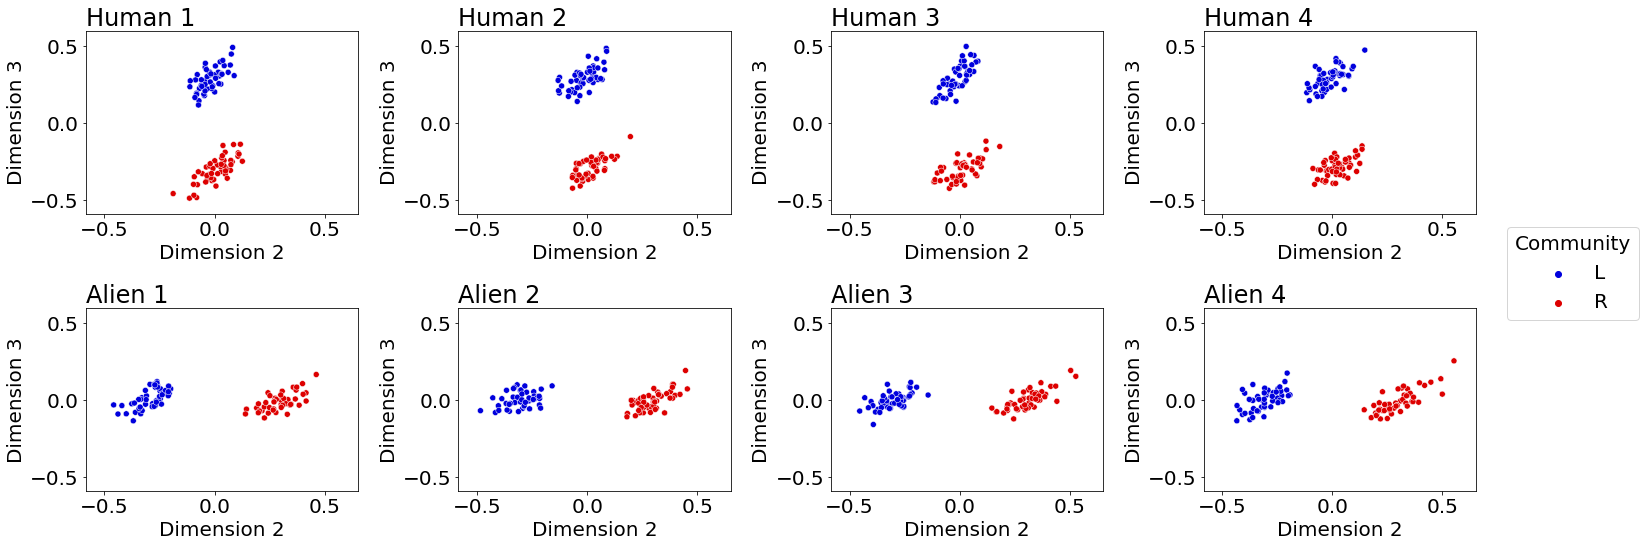
\includegraphics[width=\linewidth]{representations/ch6/Images/omni_ind.png}
    \caption[OMNI estimated latent positions]{The estimated latent positions for each network.}
    \label{fig:ch6:multinet:omni:individual}
\end{figure}

\paragraph*{Using \texttt{omni} in practice}

The procedure for the \texttt{omni} embedding is outlined in Algorithm \ref{alg:ch6:omni}. 



\begin{algorithm}[h]\caption{Omnibus Embedding (\texttt{omni})}
\label{alg:ch6:omni}
\KwData{$A^{(1)}, ..., A^{(M)}$ a collection of $M$ networks with $n$ nodes.\newline $d$ the desired latent dimensionality.}
\KwResult{estimated latent positions for each network.}
\SetAlgoLined

Compute the $Mn \times Mn$ omnibus matrix $O$, where each $n \times n$ submatrix $O^{(i,j)} = \frac{1}{2}\left(A^{(i)} + A^{(j)}\right)$.

Embed the omnibus matrix to produce estimated latent positions for the omnibus network, $\hat X = \texttt{ase}(O, d)$, according to Algorithm \ref{alg:ch6:ase}. 

Let $\hat X^{(i)}$ be the $n \times d$ matrix consisting of the $(i - 1)\cdot n + 1$ through $i\cdot n$ rows of $\hat X$.

\Return{$\hat X^{(1)}, \hdots, \hat X^{(M)}$}
\end{algorithm}

You can run \texttt{omni} using \texttt{graspologic}, as:

\begin{lstlisting}[style=python]
from graspologic.embed import OmnibusEmbed as omni

# obtain a tensor of the estimated latent positions
Xhat_tensor = omni(n_components=int(np.log2(n))).fit_transform(As)
# obtain the estimated latent positions for the first human
# network
Xhat_hum1 = Xhat[0,:,:]
\end{lstlisting}

\subsubsection{Relating \texttt{omni} to heterogeneous collections of RDPGs}

Recall from Chapter \ref{sec:ch5:multi} that a heterogeneous collection of random networks was a collection $\left\{\mathbf A^{(1)}, \hdots, \mathbf A^{(M)}\right\}$ where the underlying probability matrices $\left\{P^{(1)}, \hdots, P^{(M)}\right\}$ are not all the same. Therefore, for at least two networks $i$ and $j$, $P^{(i)} \neq P^{(j)}$.

If you think that a heterogeneous collection of random networks are each reasonably described by positive semi-definite probability matrices $P^{(i)}$, the underlying network model is that each random network $\mathbf A^{(i)}$ is an $RDPG_n\left(\mathbf X^{(i)}\right)$ random network. 

When we produced an embedding of each network using \texttt{omni}, what we did was we produced estimates $\hat X^{(i)}$ for each of our $M$ networks. 

With this framework in mind, the estimates $\hat X^{(i)}$ are interpretable as estimates of latent position matrices for each network $i$, and we can evaluate the estimated probability matrix $\hat P^{(i)} = \hat X^{(i)} \hat X^{(i)}^\top$. 

Using \texttt{omni}, you can obtain the estimates of probability matrices like this:

\begin{lstlisting}[style=python]
Phat_hum1 = Xhat_hum1 @ Xhat_hum1.T
\end{lstlisting}

Repeating this for both human and alien networks, you should be able to convince yourself that this conceptual model does a reasonable job of estimating the underlying probability matrices for our networks, like we did for \texttt{mase}.

\subsection{When should you use \texttt{omni} versus \texttt{mase}?}

Both \texttt{omni} and \texttt{mase} will produce estimated latent representations of collections of networks that will allow you to compare these estimated latent representations downstream in your analysis. In this sense, these techniques take a collection of networks, and tabularize them in such a way that you can compare the tabularized representations of the networks with tabular machine learning strategies. 

Note that \texttt{mase} effectively summarizes each network individually prior to the construction of the joint matrix, by first taking the \texttt{ase} of each individual network. The joint matrix is an $n \times Md$ matrix, where $d$ is the number of embedding dimensions that you use in the \texttt{ase} sub-step of \texttt{mase} (and is usually taken to be $\log_2(n)$). This matrix is rather manageable in size/scale for successive operations, as the number of elements is scaling on the order of $n\sqrt n$ and $M$.

\texttt{omni} has as substantial limitation: the construction (and embedding) of the omnibus matrix. The omnibus matrix scales in size with $(Mn)^2$, which can get quite computationally expensive very quickly. When you have many networks and $M$ is large, or when you have many nodes per network and $n$ is large, this can be quite computationally prohibitive to analyze. The \texttt{svd} can be quite intensive to compute with sizable matrices, and therefore in practice you might find \texttt{mase} to be simpler to incorporate into your analysis without having to make these computational considerations.

Both \texttt{omni} and \texttt{mase} are fairly simple to use, and have very similar theoretical underpinnings (\texttt{mase} on the COSIE model, and \texttt{omni} on the heterogeneous RDPG model), and are relatively intuitively flexible. While the COSIE model makes explicit use of shared structure, there is nothing prohibiting the COSIE model from incorporating little to no shared structure across your collection of networks (if none is present). We could imagine a situation where in the worst case where there is no shared structure, the estimated ``shared'' latent positions could be taken to be unique latent positions for each network. Then, the score matrices for each network could leverage only the unique latent positions for that specific network (and simply have scores of $0$ for the estimated shared latent positions that are associated with other networks). For this reason, when you want to exploit or highlight shared/unique structures across your collection of networks, \texttt{mase} is a very sensible choice to use.

A nice feature of \texttt{omni} is that it produces latent position estimates for each network, rather than just unique score matrices for each network. This means that for each network, you end up with a $d$-dimensional representation for each node. If you want to learn about disparities across your networks downstream at the node-wise level, this might be a very reasonable starting point for your analysis, and might be more direct to incorporate with tabular machine learning techniques that you are already familiar with.

For these reasons, our advice would be, if computational time or spatial considerations need to be made, or if you anticipate some amount of shared structure in your networks, \texttt{mase} might be more reasonable to use for your analysis. If you do not anticipate shared structure in your networks, either \texttt{mase} or \texttt{omni} are principled approaches to proceeding, and you could identify a strategy on the basis of the representation (estimated shared latent position matrices and unique score matrices, or unique estimated latent positions) that you are most comfortable working with.

\newpage
\section{Joint representation learning}
\label{sec:ch6:joint}

In many problems, our network might be more than just the information contained in its adjacency matrix (called its \textit{network topology}, or its collection of nodes and edges). If we were investigating a social network, we might have access to extra information about each person -- their gender, for instance, or their age. If we were investigating a brain network, we might have information about the physical location of neurons, or some notion of how big a brain region is. When we embed a network, it seems like we should be able to use these extra bits of information - called the ``features'' or ``covariates'' of the nodes in the network - to somehow improve our analysis. The techniques and tools that we'll explore in this section use both the covariates and the topology of a network to create and learn from new representations of the network. Because they jointly use both the topology of the network and its extra covariate information, these techniques and tools are called joint representation learning.

There are two primary reasons that we might want to explore using node covariates in addition to topological structure. First, they might improve our standard embedding algorithms, like Laplacian and Adjacency Spectral Embedding. For example, if the latent structure of the covariates of a network lines up with the latent structure of its topology, then we might be able to reduce noise when we embed, even if the communities in our network don't overlap perfectly with the communities in our covariates. Second, figuring out what the clusters of an embedding actually mean can sometimes be difficult and covariates create a natural structure in our network that we can explore. Covariate information in brain networks telling we where in the brain each node is, for instance, might let us better understand the types of characteristics that distinguish between different brain regions.

In this section, we'll explore different ways to learn from our data when we have access to the covariates of a network in addition to its topological structure. we'll explore \textit{Covariate-Assisted Spectral Embedding} (\texttt{case}), a variation on Spectral Embedding developed by \cite{Binkiewicz2017Jun}. In \texttt{case}, instead of embedding just the adjacency matrix or its Laplacian, we will combine the Laplacian and our covariates into a new matrix and embed that.

\begin{floatingbox}[h]\caption{School network example}
A good way to illustrate how using covariates might help us is to use a model in which some of our community information is in the covariates and some is in our topology. Let's imagine we have a network of $N=200$ nodes representing wikipedia pages for two complementary fields; computer science and statistics. A pair of wikipedia pages have an edge if both of the wikipedia pages link to one another. 

Unfortunately in our network, there is an extremely strong and prominent core: the top $50$ computer science wikipedia pages and the top $50$ statistics wikipedia pages tend to overwhelmingly cross-link to one another, and do not tend to link to the peripheral, more specialized, pages nearly as much.

When you attempt to embed this network via a strategy you have learned already like \texttt{ase}, you will likely be able to yield an embedding differentiate the strong core very easily from the periphery, but you will struggle to parse out the ``subject-matter specific'' signal of retaining the differences between computer science and statistics articles.

Fortunately, you also have another piece of information: whether a given page cites each of the twenty most influential statisticians of all time. This is a simple indicator for each statistician; a value of $1$ is recorded for page $i$ and statistician $k$ if statistician $k$ is cited by page $i$.
\end{floatingbox}

Let's first generate the network data for the wikipedia pages:

\begin{lstlisting}[style=python]
import numpy as np


n = 200  # total number of nodes
# first two communities are the ``core'' pages for statistics
# and computer science, and second two are the ``peripheral'' pages
# for statistics and computer science.
B = np.array([[.4, .3, .05, .05],[.3, .4, .05, .05],[.05, .05, .05, .02],[.05, .05, .02, .05]])

# make your stochastic block model
A, labels = sbm([n // 4, n // 4, n // 4, n // 4], B, return_labels=True)
# generate labels for core/periphery
co_per_labels = ["Core" for i in range(n // 2)] + ["Periphery" for i in range(n // 2)]
# generate labels for statistics/CS
st_cs_labels = ["Stat" for i in range(n // 4)] + ["CS" for i in range(n // 4)] + \
            ["Stat" for i in range(n // 4)] + ["CS" for i in range(n // 4)]
\end{lstlisting}

The network is shown in Figure \ref{fig:ch6:casc:casc_net}(A). We show the results of a \texttt{lse} of the network into two dimensions in Figure \ref{fig:ch6:casc:casc_net}(B). Note that embedding this network, we can only do a decent job of distinguishing the core nodes (from both CS and Statistics) from the periphery nodes (from both CS and Statistics), but we cannot differentiate between the two subject materials.

\begin{figure}[h]
    \centering
    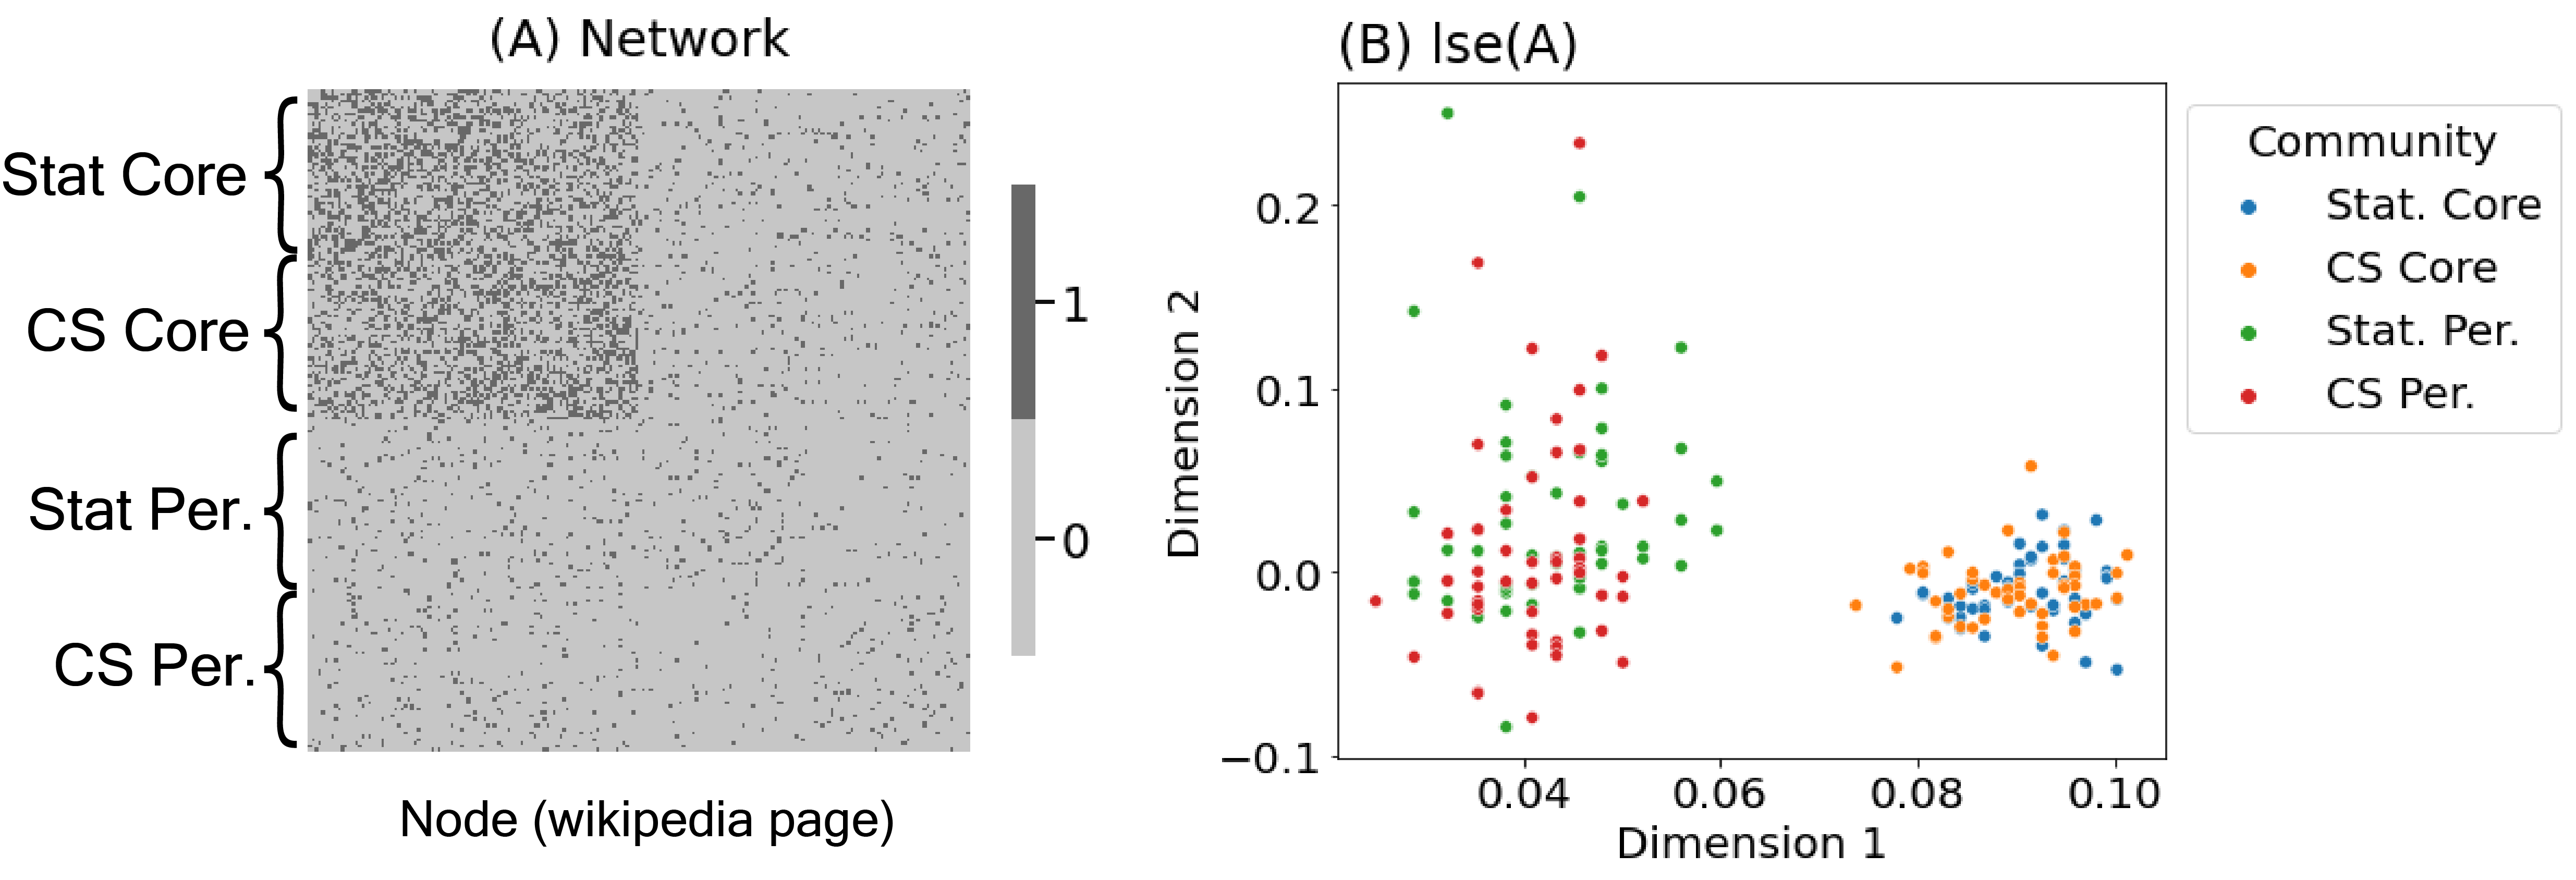
\includegraphics[width=\linewidth]{representations/ch6/Images/casc_net.png}
    \caption[\texttt{CASC} network]{\textbf{(A)} the wikipedia network, \textbf{(B)} a \texttt{lse} of the wikipedia network.}
    \label{fig:ch6:casc:casc_net}
\end{figure}

Next, we'll focus on generating the covariates associated with each node. We have a simple binary indicator for each page, indicating whether any of our twenty influential statisticians are cited. For statistics pages, there is a $50\%$ change that each of the twenty statisticians are cited. However, for computer science pages, there is only a $5\%$ chance that any of the three statisticians are cited. We can generate these covariates like this, using \texttt{numpy}:

\begin{lstlisting}[style=python]
trial = []
for label in st_cs_labels:
    if "Stat." in label:
        # if the page is a statistics page, there is a 40% chance
        # of citing each of the scholars
        trial.append(np.random.binomial(1, 0.5, size=20))
    else:
        # if the page is a CS page, there is a 5% chance of citing
        # each of the scholars
        trial.append(np.random.binomial(1, 0.05, size=20))
Y = np.vstack(trial)
\end{lstlisting}

The covariate matrix is plotted in Figure \ref{fig:ch6:casc:cov_repr}(A). Next, we perform a \texttt{pca} with the covariates, to determine whether we could learn the four communities (core and periphery of statistics and computer science) using only the covariate data:

\begin{lstlisting}[style=python]
def embed(X, d=2):
    """
    A function to embed a matrix.
    """
    Lambda, V = np.linalg.eig(X)
    return V[:, 0:d] @ np.diag(np.sqrt(np.abs(Lambda[0:d])))

def pca(X, d=2):
    """
    A function to perform a pca on a data matrix.
    """
    X_centered = X - np.mean(X, axis=0)
    return embed(X_centered @ X_centered.T, d=d)

Y_embedded = pca(Y, d=2)
\end{lstlisting}
We plot the resulting embedding in Figure \ref{fig:ch6:casc:cov_repr}(B). note that this time, we have excellent separation of the statistics and computer science pages, but we cannot differentiate the core from the periphery.

\begin{figure}[h]
    \centering
    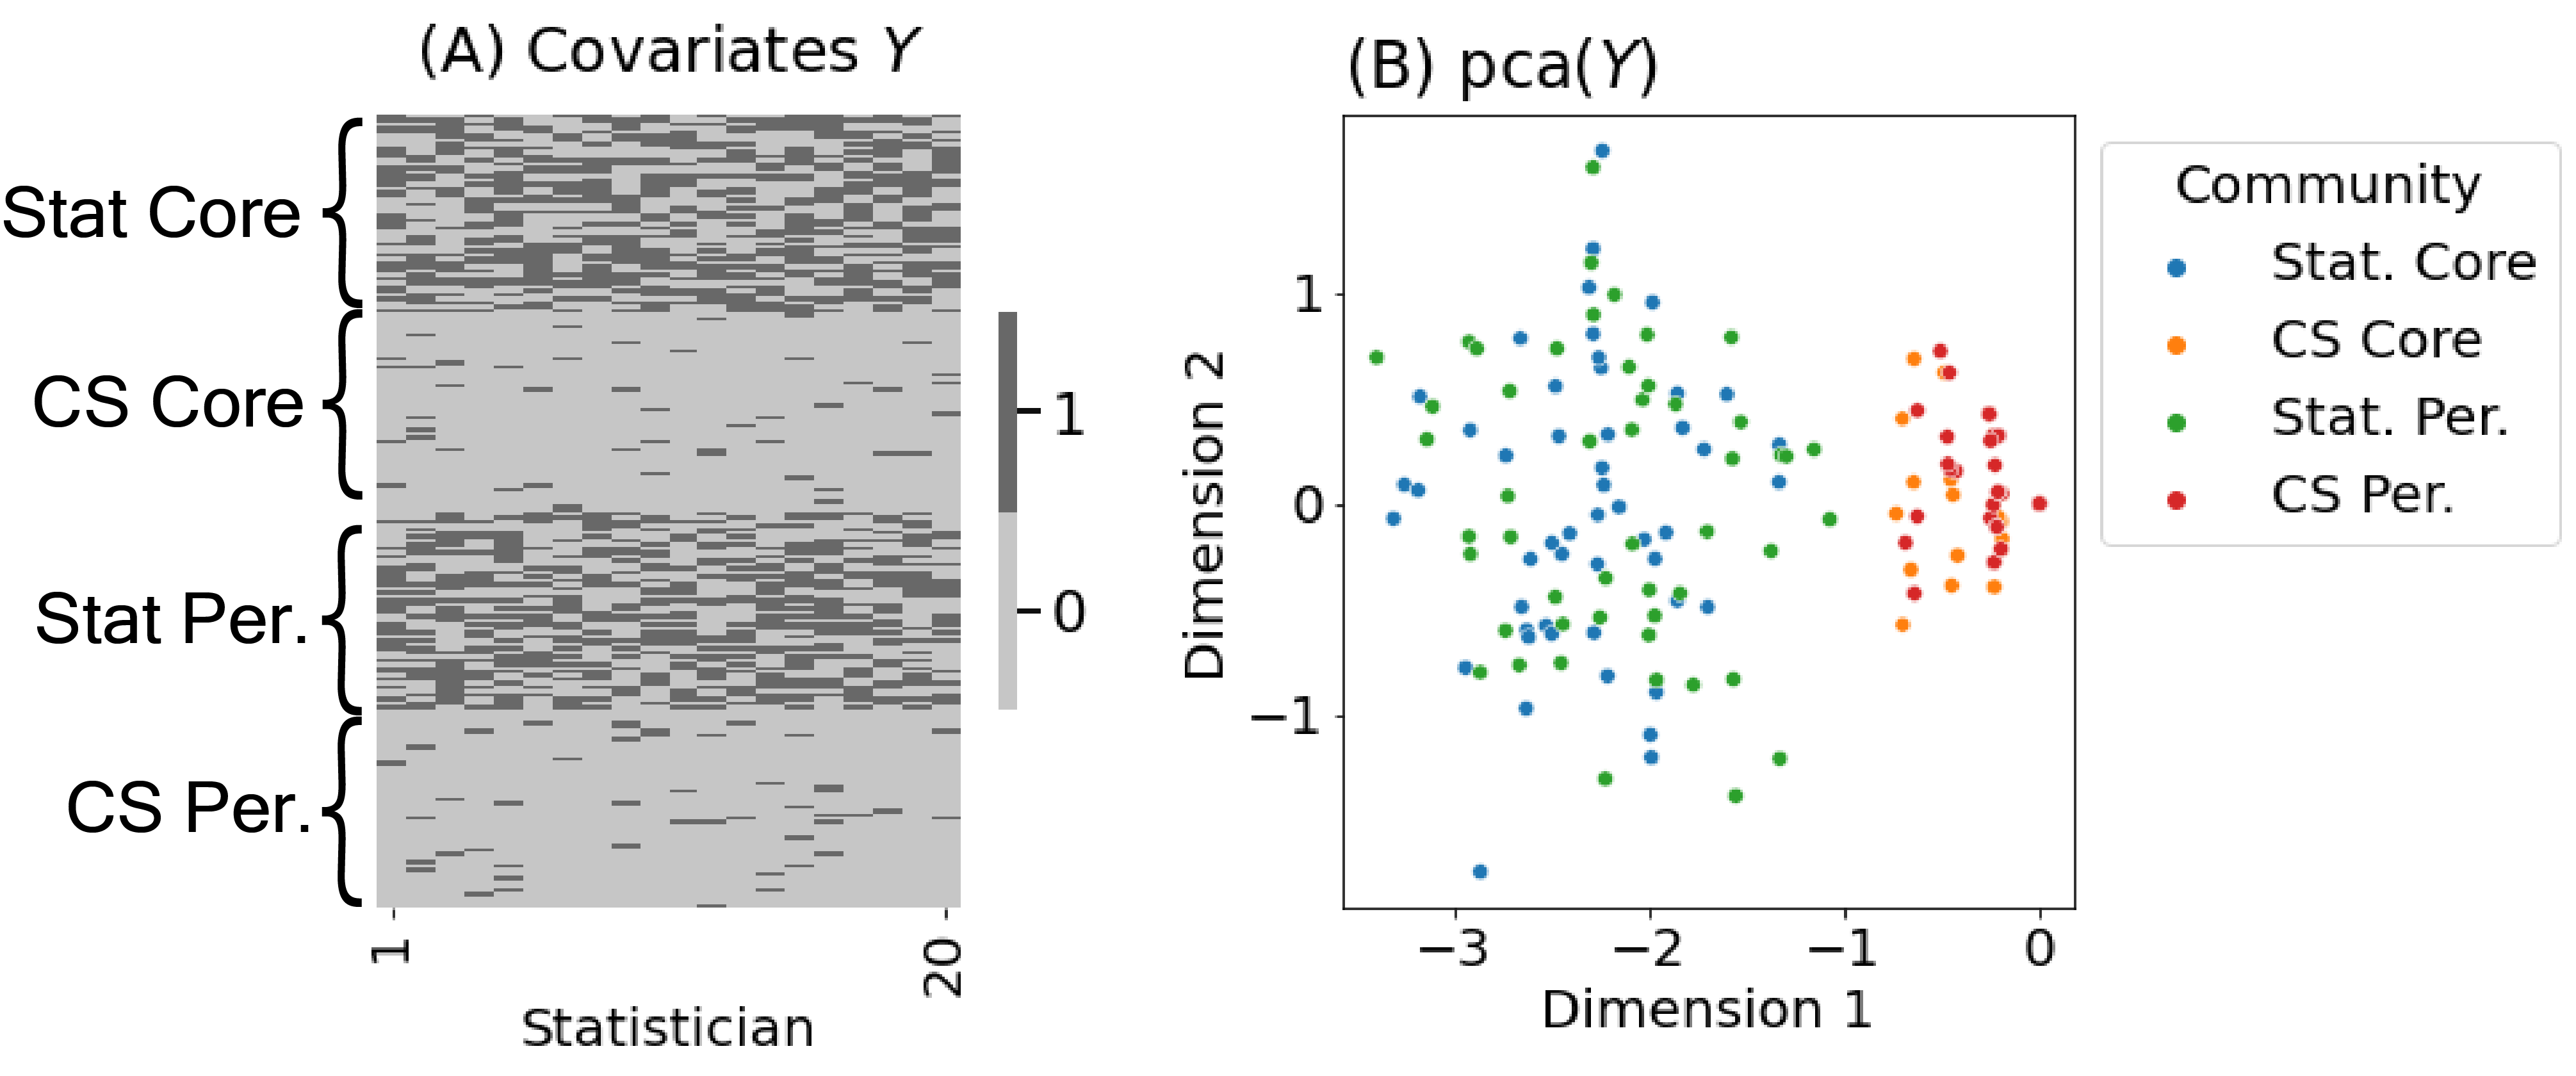
\includegraphics[width=\linewidth]{representations/ch6/Images/casc_covs.png}
    \caption[\texttt{pca} of covariates]{\textbf{(A)} the covariates associated with each wikipedia page, \textbf{(B)} a \texttt{pca} of the covariate data.}
    \label{fig:ch6:casc:cov_repr}
\end{figure}

\subsection{Covariate-Assisted Spectral Embedding}

\textit{Covariate-Assisted Spectral Embedding}, or \texttt{case}, is a simple way of combining our network and our covariates into a single model. In the most straightforward version of \texttt{case}, we take a weighted combination of the network's Laplacian $L$ and a similarity matrix for our covariates, $YY^\top$. 

\begin{floatingbox}\caption{Connections to Principal Components Analysis (\texttt{pca})}
\label{box:ch6:casc:pca}
If you have studied machine learning previously, this matrix should look familiar to you.

Note that the rows of the matrix $Y$, denoted by $\vec y_i$, are each $20$-dimensional vectors, where each entry has a value of $0$ of $1$. The matrix product $YY^\top$ has entries:
\begin{align*}
    (YY^\top)_{ij} = \vec y_i^\top \vec y_j = \sum_{k = 1}^{20} y_{ik}y_{jk}.
\end{align*}
In this case, since the values of our covariate matrix can take only $0$s and $1$s, this basically just counts up the number of times wikipedia page $i$ and wikipedia page $j$ both cite scholar $k$. In this sense, you can conceptualize the uncentered, un-rescaled covariance matrix $YY^\top$ as giving a degree of ``similarity'' in the covariates for each of our nodes. 

Much like \texttt{ase} exploits latent behaviors in the adjacency matrix to determine an appropriate embedding, a \texttt{pca} exploits latent behaviors in the covariances of our data matrix (here, our covariates, $Y$) to embed a given dataset. Typically, \texttt{pca} would spectrally embed the centered and scaled covariance matrix:
\begin{align*}
    \frac{1}{n - 1}\left(Y - \vec \mu_y\right)\left(Y - \vec \mu_y\right)^\top
\end{align*}
This is distinct from the procedure that we are using here, because we will not typically take the centering nor the scaling steps (but, we certainly could).
\end{floatingbox}

Let's take a look at what the network Laplacian and the covariate similarity matrix $YY^\top$ look like here:

\begin{lstlisting}[style=python]
from graspologic.utils import to_laplacian

# compute the network Laplacian
L_wiki = to_laplacian(A, form="DAD")
# log transform, strictly for visualization purposes
L_wiki_logxfm = np.log(L_wiki + np.min(L_wiki[L_wiki > 0])/np.exp(1))

# compute the node similarity matrix
Y_sim = Y @ Y.T
\end{lstlisting}

The network Laplacian and the node similarity matrix are shown in Figure \ref{fig:ch6:casc:casc_inputs}. Note that we used the log-transforming strategy from Section \ref{fig:ch4:log_xfm} to visualize the log-transformed Laplacian after adding a suitably small offset $\epsilon$, as many of the network weights were extremely small, so the color scale was not particularly informative on the Laplacian itself (try plotting it yourself).

\begin{figure}
    \centering
    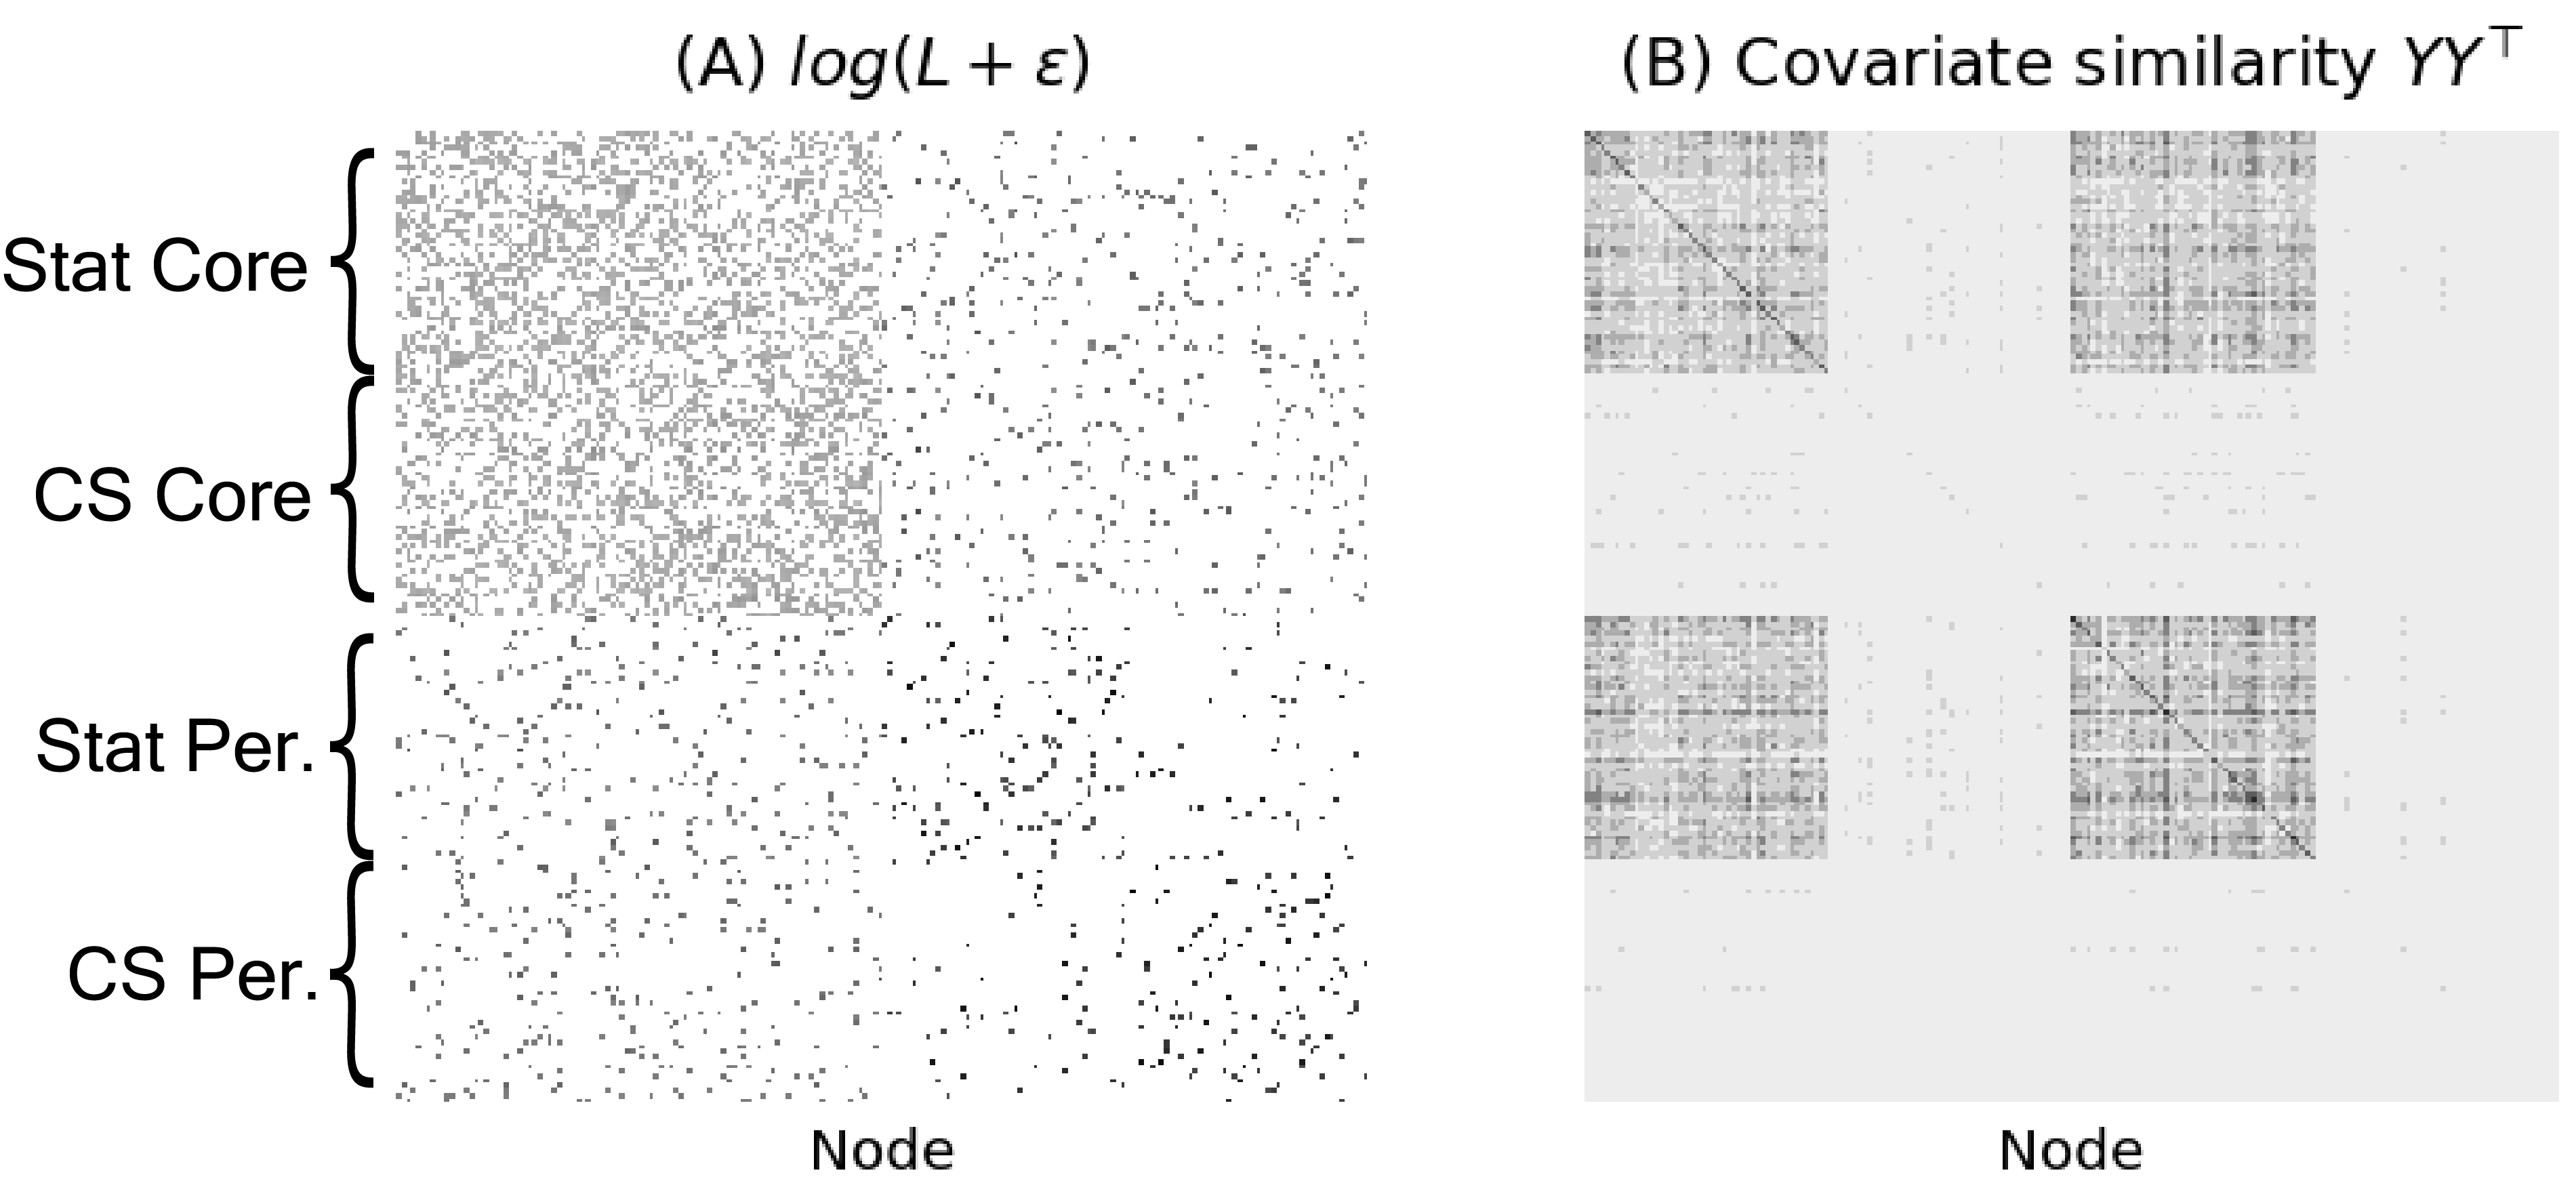
\includegraphics[width=\linewidth]{representations/ch6/Images/casc_inputs.png}
    \caption[inputs to \texttt{case}]{\textbf{(A)} a visualization of the log-transformed network Laplacian, and \textbf{(B)} the covariate similarity matrix.}
    \label{fig:ch6:casc:casc_inputs}
\end{figure}

Note that each embedding appears to preserve disparate properties about the underlying network: the topology of the network, reflected in the network Laplacian, conveys the topological disparities between the core and peripheral pages in our network. On the other hand, the covariate metadata that we have associated with each node in the network conveys the content disparities between the statistics and computer science nodes in the network. 

\paragraph*{Combining information from the network topology and the covariates}

The matrix that is spectrally embedded through \texttt{case} is a linear combination of the network Laplacian $L$ and the covariate similarity matrix $YY^\top$. It is typically represented like this:
\begin{align*}
    L + \alpha YY^\top.
\end{align*}
The weight $\alpha$ is a hyper-parameter to the \texttt{case} technique, in that it is a parameter that we will often want to select with respect to a downstream task of interest. 

\begin{lstlisting}[style=python]
from graspologic.embed import AdjacencySpectralEmbed

def case(A, Y, weight=0, d=2, tau=0):
    """
    A function for performing case.
    """
    # compute the laplacian
    L = to_laplacian(A, form="R-DAD", regularizer=tau)
    YYt = Y @ Y.T
    return AdjacencySpectralEmbed(n_components=2)(L + weight*YYt)

embedded = case(A, Y, weight=.002)
\end{lstlisting}

For instance, if we had a high-level goal of producing an embedding which preserved both topological properties of the network (such as the core and peripheral components) as well as covariate-derived properties of the network (such as statistics and computer science components), a heuristic might be to try numerous weights $\alpha$, and evaluate the resulting embeddings for each choice of $\alpha$. A suitable choice of $\alpha$ would be a choice in which the community groupings are preserved.

\begin{figure}[h]
    \centering
    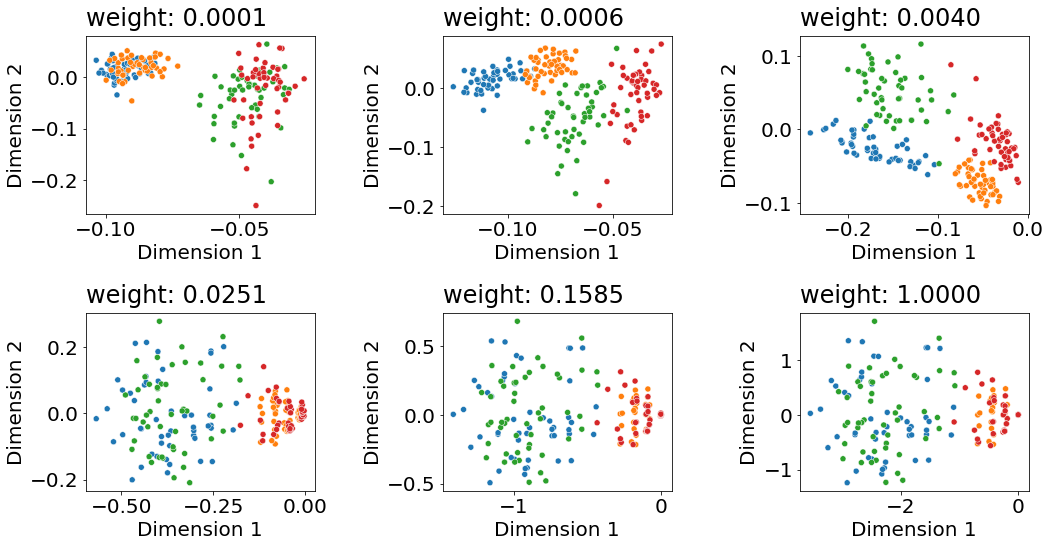
\includegraphics[width=\linewidth]{representations/ch6/Images/case_outputs.png}
    \caption[CASE embedding example]{The network embedding using both the network topology and the node covariates, for different choices of $\alpha$.}
    \label{fig:ch6:casc:casc_out}
\end{figure}
Figure \ref{fig:ch6:casc:casc_out} explores various network embeddings with different choices of $\alpha$. Note that for low choices of $\alpha$, the embedding resembles that of the topology only \texttt{lse} in Figure \ref{fig:ch6:casc:casc_net}(B). For large choices of $\alpha$, the embedding closely resembles that of the covariate-only embedding in Figure \ref{fig:ch6:casc:cov_repr}(B). For the intermediate choices, such as $\alpha = .0006$ or $\alpha = .004$, the embedding appears to leverage information across both the covariates and the network topology, and both the core/periphery and subject matter (statistics/computer science) structures are preserved.

\subsubsection{Automatic weight selection}

In general, it is ideal to perform joint representation learning with an approach like \texttt{case} with a downstream machine learning task in mind. This is because the weight selection procedure of \texttt{case} is a search over hyperparameters, and it is difficult to determine what an appropriate hyperparameter choice is without any way to evaluate your hyperparameter. For instance, in the evaluation above, we determined ``ideal'' weight selections to be on the basis of how well different weights established community structure for known communities. We could make such a search more quantitative by incorporating a procedure which quantifies ``community separation'' between groups of nodes.

While we cannot automatically determine an ``ideal'' weight in terms of an arbitrary downstream task that you might have, we can take principled steps to ensure that the two components of \texttt{case} (the normalized Laplacian and the covariate similarity matrix) are contributing relatively equally to the embedding process.

When you embed symmetric matrices, keep in mind that the actual points you’re plotting are the components of the eigenvectors with the biggest eigenvalues. When you embed into two-dimensional space, for instance, the $x$-axis values of your points are the components of the eigenvector with the biggest eigenvalue, and the $y$-axis values are the components of the eigenvector with the second-biggest eigenvalue. This means that you should probably be thinking about how much information the Laplacian and contributes to the biggest eigenvalue/eigenvector pairs.

Thinking about this more, if you have a small weight, $YY^\top$ will contribute only a small amount to the biggest eigenvalue/vector pair. If you have a large weight, $YY^\top$ will contribute a large amount to the biggest eigenvalue/vector pair. A roughly prudent starting point for your embedding, therefore, might be the ratio of the biggest eigenvalue of $L$ and the biggest eigenvalue of $YY^\top$:

\begin{align*}
\alpha_0 = \frac{\lambda_1 (L)}{\lambda_1 (YY^\top)}    
\end{align*}

The \texttt{case} procedure can be automated in \texttt{graspologic}, with:

\begin{lstlisting}[style=python]
from graspologic.embed import CovariateAssistedEmbed as case

embedding = case(alpha=None, n_components=2).fit_transform(A, covariates=Y)
\end{lstlisting}
To specify a specific weight, you can do so with the \texttt{alpha} parameter.

\subsection{Considerations for positive semi-definiteness}

As we will see in Section \ref{sec:ch6:dimest:grdpg}, most of the techniques discussed thus far theoretically operate well under a relatively homogeneous setting captured by the gRDPG. This setting extends the intuition of what we have discussed (which, conceptually, we tended to stick to the positive semi-definite case) to the non positive semi-definite case. 

\texttt{case} operates a bit on its own compared to the other algorithms described in this section, and does not quite fall into the same theoretical framework (despite sharing many conceptual and intuitive similarities). In the situation where you have reason to believe that the random network underlying your experiment is not positive semi-definite, such as if you are able to identify a disassortative block structure (from Section \ref{sec:ch5:psd_block}), you can alter your Laplacian to be positive semi-definite by simply instead embedding $LL + \alpha YY^\top$. This can be done in \texttt{graspologic} with:

\begin{lstlisting}[style=python]
embedding = case(assortative=False, n_components=2).fit_transform(A, covariates=Y)
\end{lstlisting}

When you are not sure whether the structure of your network supports positive semi-definite or non positive semi-definite structure in the underlying random network, the authors advise \cite{Binkiewicz2017Jun} that non-assortative \texttt{case} tends to perform nearly as well under assortative structures, and far better under non-assortative structures.

\subsection{Extensions of \texttt{case}}

In this section, we introduced a relatively simple technique for augmenting our typical \texttt{lse} algorithm for the case where we had node-specific covariate information. We accomplished this via a matrix $YY^\top$, which we combined (with a suitable weight parameter) with our Laplacian.

That said, an extension that you might have is to consider other possible similarity functions (other than simply the inner product $\vec y_i^\top \vec y_j$) that you might use for covariate assisted embedding techniques. For instance, \texttt{graspologic} also allows centering and scaling steps to be taken, in much the same vein as the typical pre-processing steps for \texttt{pca}. You could further generalize this strategy to other similarity functions entirely. In your work, you may be motivated to define other similarity criteria that go beyond this approach that was originally used in \cite{Binkiewicz2017Jun} to devise new approaches for covariate-assisted spectral embeddings.


\newpage
\section{Estimating latent dimensionality and non positive semi-definiteness}
\label{sec:dimest}

\subsection{The problem of estimating latent dimensionality}
\label{sec:ch6:dimest:dimselect}
Across all of the embedding techniques we have discussed thus far, we typically have ignored a relatively substantial problem. In all of these algorithms, a hyperparameter for the embedding technique has, in general, been the latent dimensionality $d$. 

The latent dimensionality is associated with the latent dimensionality of an underlying random network, $\mathbf A$. It is important to clarify that this random network has no real interpretation; it only exists for conceptual (being able to think about what is going on) and theoretical (being able to prove that the embedding approach is reasonable in some concrete context) sake. Without knowing a suitable latent dimensionality $d$, this theoretical and intuitive insight starts to break down. For this reason, it is fairly imperative that we are able to in practice make reasonable guesses about $d$; using the notation we have become accustomed to by this point, we need to be able to estimate it with $\hat d$. 

Let's get a working example together:

\begin{lstlisting}[style=python]
from graspologic.simulations import sbm
import numpy as np

# block matrix
n = 100
B = np.array([[0.6, 0.2], [0.2, 0.4]])
# network sample
A, z = sbm([n // 2, n // 2], B, return_labels=True)
\end{lstlisting}

\subsection{The scree plot}

Throughout any investigation into spectral embeddings, one of the critical summary statistics to look at with respect to your embedding matrix (the matrix being embedded) is its scree plot. 

The \textit{scree plot} is a plot of the singular values of the embedding matrix (the diagonal entries of the singular value matrix $\Sigma$) in sequential (descending) order by their indices: the first (biggest) singular value is in the beginning, and the last (smallest) singular value is at the end. You can get the singular values like this:

\begin{lstlisting}[style=python]
from scipy.linalg import svdvals

# use scipy to obtain the singular values
s = svdvals(A)
\end{lstlisting}

And you can look at the scree plot like this:

\begin{lstlisting}[style=python]
from pandas import DataFrame
import seaborn as sns
import matplotlib.pyplot as plt


def plot_scree(svs, title=""):
    """
    A utility to plot the scree plot for a list of singular values
    svs.
    """
    if ax is None:
        fig, ax = plt.subplots(1,1, figsize=(10, 4))
    sv_dat = DataFrame({"Singular Value": svs, "Dimension": range(1, len(svs) + 1)})
    sns.scatterplot(data=sv_dat, x="Dimension", y="Singular Value", ax=ax)
    sns.lineplot(data=sv_dat, x="Dimension", y="Singular Value", ax=ax)
    ax.set_xlim([0.5, len(s)])
    ax.set_title(title)

plot_scree(s, title="Scree plot of $L$")
\end{lstlisting}

The scree plot is shown in Figure \ref{fig:ch6:scree}(A). Essentially, the intuition is this: the singular values correspond to the relative amount of ``information'' for each singular vector (left or right) in describing the matrix that you are embedding. Since the singular values are decreasing ($\sigma_1 \geq \sigma_2 \geq ... \geq \sigma_n \geq 0$, as we discussed above) each sequential singular value is less and less important for describing the network that you have embedded. In Figure \ref{fig:ch6:scree}(B), we isolate out the first ten dimensions from this plot.

\begin{figure}[h]
    \centering
    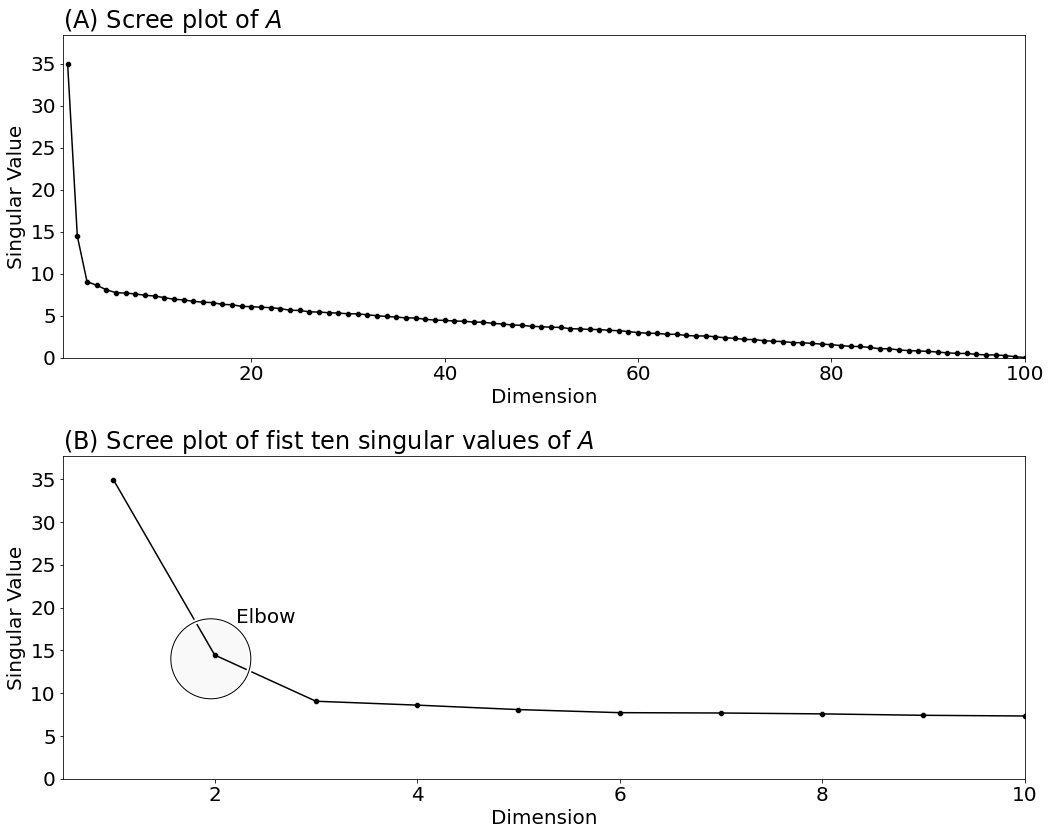
\includegraphics[width=\linewidth]{representations/ch6/Images/scree.png}
    \caption[Scree plot of an adjacency spectral embedding]{\textbf{(A)} the scree plot of singular values of $A$, and \textbf{(B)} the scree plot of the first ten singular values of $A$, with the elbow annotated.}
    \label{fig:ch6:scree}
\end{figure}

You'll notice that there's a marked area called the ``elbow''. This is an area where singular values stop changing in magnitude as much when they get smaller: before the elbow, the singular values decline rapidly, and after the elbow, the singular values ``level off''. It is called an elbow because the plot kind of looks like an arm, viewed from the side.

The location of this elbow gives you a rough indication for how many ``true'' dimensions your latent representation has. The singular values after the elbow are quite close to each other and have singular vectors which are largely noise, and don't tell you very much about your data. It looks from the scree plot that you should be embedding down to two dimensions, as the smaller dimensions tend to be more "noisy" than the first few. The first few will tend to do a good job of describing the overall structure of the matrix that you have embedded, whereas successive dimensions tend to not be as useful. Notice that our example $SBM_n(\vec z, B)$ random network has a true latent position matrix with two latent dimensions, by using the results we obtained in Section \ref{sec:ch5:psd_block:lpm_fromsbm}. This coincides with the location of the elbow on the scree plot for the network sample $A$, so we were able to effectively estimate the true latent dimensionality $d$ using only the data sample $A$. 

\paragraph*{The balancing act of elbow selection}

Particularly when networks have fewer nodes, or when your adjacency matrix has very few non-zero entries, this tends to get rather messy. There may be multiple elbows in your scree plot, and it may be unclear where you should ``draw the line'' and cut off extraneous singular values. By removing too many dimensions, you may end up cutting off dimensions that contain latent structure in your estimated latent positions that you could use downstream to learn about your network. By removing too few dimensions, you may be left with estimated latent positions that have too many latent dimensions, and learning about your network later might be overly complicated. In this sense, there is a balancing act to choosing an estimated latent dimensionality.

\subsection{Automatic elbow selection}

Another drawback to the visual method of estimating latent dimensionality is that a lot of the time, the elbow location is fairly subjective. Real data will rarely have a prominent like the simulated network you see above. The advantage is that it still generally works pretty well; embedding into a few more dimensions than you need isn't too bad, since you'll only have a few noise dimensions and there still may be *some* signal there.

\texttt{graspologic} automates the process of finding an elbow using a popular method developed in 2000 by Dr. Thomas Minka at MIT (called \texttt{minka}, from \cite{Minka2000}). We won't get into the specifics of how it works here, but it generally does a fairly good job at automatic elbow selection. When you use any embedding methods and do not specify a number of embedding dimensions (via the \texttt{n\_components} argument that we used throughout this section), the elbow selection is done automatically:

\begin{lstlisting}[style=python]
from graspologic.embed import AdjacencySpectralEmbed as ase

# use automatic elbow selection
Xhat_auto = ase().fit_transform(A)
\end{lstlisting}

Looking at the number of columns of \texttt{Xhat\_auto.shape[1]} gives you the dimensionality estimated by graspologic. 


\subsection{What happens for non positive semi-definite probability matrices?}
\label{sec:ch6:dimest:grdpg}

\paragraph*{Why did we ignore non positive semi-definite probability matrices?}

Throughout this book, we have taken an overarching intuitive leap: we have conceptualized the underlying random networks to have positive semi-definite probability matrices. This has some extremely convenient implications for us. 

First, we were able to bridge latent position matrices with $DCSBM_n(\vec z, \vec \theta, B)$ and $SBM_n(\vec z, B)$ random networks with positive semi-definite block matrices exactly and succinctly, taking the probability matrices to be:
\begin{align*}
    P_{sbm} &= C B C^\top \\
    P_{dcsbm} &= \Theta C B C\Theta^\top
\end{align*}
where since $B$ was positive semi-definite, it had an exact square-root matrix (which was real) that we could calculate. This allowed you to obtain exact (real) representations of latent positions:
\begin{align*}
    X_{sbm} &= C\sqrt{B} \\
    X_{dcsbm} &= \Theta C \sqrt{B}
\end{align*}
Where we would always be able to compute $\sqrt{B}$ in an exact form (using the Cholesky decomposition, as we did in Section \ref{sec:ch5:psd_block}). 

Second, in order to understand the results in this Chapter, the assumptions that we needed (linear algebra wise) are comparatively easy to wrap your head around; positive semi-definiteness gave us immediate conclusions about the eigendecomposition and the singular value decomposition in Remarks \ref{box:ch6:evd_sum} and \ref{box:ch6:svd_results} respectively. You can find understandable proofs of many of the results that these remarks summarized that are (comparatively) easy to read across numerous linear algebra books \cite{Axler, Trefethen1997} or other online resources. These remarks led to immediate equality of calculations of $P$ (or the population Laplacian $\mathcal L$) using the eigendecomposition and the singular value decomposition, without needing to stray too far from background that would be gained from an introductory linear algebra course, which we believe is fairly important to being able to nail the concepts down in your head appropriately. 

Finally, positive semi-definite structure tends to arise readily in real data. It is a context that you will become very familiar with as you develop as a network machine learning scientist, and many block matrix structures that we explored in Section \ref{sec:ch5:psd_block} materialize frequently in a positive semi-definite manner. Therefore, grasping core intuition about random networks where the underlying block matrices are positive semi-definite will play an important role in your ability to conceptualize many real problems that you will come across.

\paragraph*{The generalized random dot product graph}

That said, it is important to realize that even if $P$ is not positive semi-definite, it can still be decomposed in the form \cite{Athreya2017Jan, Rubin2022Sep}:

\begin{align*}
    P &= XI_{p, q} X^\top \numberthis\label{eqn:ch6:grdpg:e1}
\end{align*}

Where $X$ is a real latent position matrix that is very similar to the latent position matrix that you have learned about before. Remember that $X$ is a $n \times d$ matrix, so $I_{p, q}$ will be a $d \times d$ square matrix. In particular, $I_{p, q}$ will be a special ``variation'' of the identity matrix. It will be a matrix of $p$ consecutive $1$s, followed by $q$ consecutive $-1$s. So, we have the restriction that $p + q = d$. 

Notice that if $p = d$, that $P = XX^\top$, so $P$ is positive semi-definite because it can be decomposed into the product of a real matrix and itself. However, if $p < d$ and consequently $q > 0$, this matrix is not necessarily positive semi-definite. 

Recent work \cite{Rubin2022Sep} has shown that even when $P$ is not positive semi-definite, \texttt{ase} can still recover estimates $\hat X$ of $X$ (up to a rotation) that are reasonable in the same sense that \texttt{ase} was reasonable for networks with underlying positive semi-definite probability matrices. Further, these latent positions $X$ share all of the convenient features that latent position matrices for positive semi-definite $SBM_n(\vec z, B)$ and $DCSBM_n(\vec z, \vec \theta, B)$ random networks in Section \ref{sec:ch5:psd_block:same_lp}. 

If the random network is an $SBM_n(\vec z, B)$ random network (positive semi-definite block matrix or not), the latent position vectors $\vec x_i$ from the decomposition in Equation \eqref{eqn:ch6:grdpg:e1} will still be the same for all nodes in the same community. If the random network is a $DCSBM_n(\vec z, \vec \theta, B)$ random network (positive semi-definite block matrix or not), the latent position vectors $\vec x_i$ from the decomposition in Equation \eqref{eqn:ch6:grdpg:e1} will also be the same (up to a rescaling by the degree-correction factor) for all nodes in the same community. 

That \texttt{ase} (and consequently, \texttt{lse}, \texttt{omni}, and \texttt{mase}) can recover estimates $\hat X$ of $X$ that are reasonable suggests that we can still use $\hat X$ to recover latent structure in the estimates of the latent positions produced with these strategies, even if positive semi-definiteness is not a reasonable assumption about the networks to make.

This way of representing $P$ given in Equation \eqref{eqn:ch6:grdpg:e1} is known as the generalized Random Dot Product Graph, or $gRDPG_n\left(X, I_{p + q}\right)$ model. This model is equivalent hierarchically in Figure \ref{fig:ch5:hierarchy} to the $IER_n(P)$ random networks, in that for every probability matrix $P$, there exists some latent position matrix $X$ that has $d \leq n$ latent dimensions  and $I_{p + q}$ where $P = XI_{p,q}X^\top$. This makes the gRDPG an extremely powerful theoretical tool for network embeddings, because it can be used to conceptualize any probability matrix. 

To motivate the utility of the \texttt{ase} outside of positive semi-definite contexts, let's see what happens when we perform \texttt{ase} on a sample of an $SBM_n(\vec z, B)$ random network with a disassortative block matrix from Section \ref{sec:ch5:psd_block}. Remember that disassortative block matrices have the off-diagonal entries necessarily greater than the on-diagonal entries, by definition, so the determinant is negative. Since the determinant could be used to characterize a $2 \times 2$ matrix as non positive semi-definite, this meant that the disassortative block matrices were non positive semi-definite:

\begin{lstlisting}[style=python]
from graspologic.embed import AdjacencySpectralEmbed as ase
from scipy.spatial import distance_matrix

nk = 50  # the number of nodes in each community
B_indef = np.array([[.1, .5], [.5, .2]])
A_dis, z = sbm([nk, nk], B_indef, return_labels=True)
Xhat = ase(n_components=2).fit_transform(A_dis)
D = distance_matrix(Xhat, Xhat)
\end{lstlisting}

\begin{figure}[h]
    \centering
    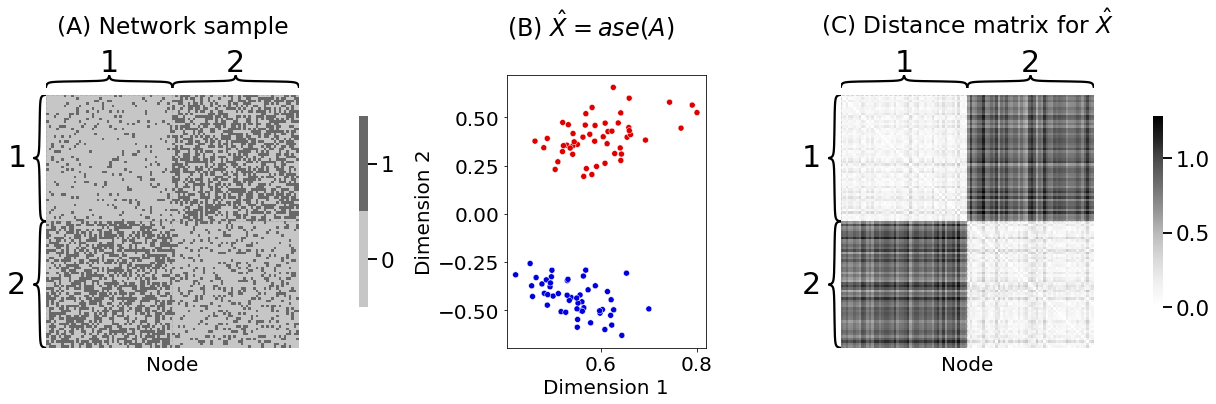
\includegraphics[width=\linewidth]{representations/ch6/Images/diss.png}
    \caption[ASE with indefinite probability matrix]{\textbf{(A)} a sample of a random network with an indefinite block matrix, and hence, and indefinite probability matrix, \textbf{(B)} a scatter plot of the estimated latent positions via \texttt{ase}, \textbf{(C)} the distance matrix between pairs of estimated latent positions.}
    \label{fig:ch6:dimest:diss}
\end{figure}

We visualize the sample of the random network with a non positive semi-definite probability matrix in Figure \ref{fig:ch6:dimest:diss}(A), where it is fairly evident that between-community connections (the off-diagonal blocks of the adjacency matrix in the upper-right and lower-left corners) are more frequent than within-community connections (the on-diagonal blocks of the adjacency matrix). This intuitively reflects the idea that the underlying random network has a non positive semi-definite probability matrix. The estimated latent positions are shown in Figure \ref{fig:ch6:dimest:diss}(B). Notice that even though the block matrix (and consequently the probability matrix) of the underlying random network is not positive semi-definite, that \texttt{ase} still produced a meaningful embedding, in that nodes from the same community were still more similar than nodes from different communities. This insight can be confirmed by looking at the pairwise distance matrix, in Figure \ref{fig:ch6:dimest:diss}(C). While some of the strategies discussed, such as the \texttt{omni} embedding \cite{Levin2017}, were developed prior to these results, it is likely that they produce principled estimates of latent positions even under non positive semi-definite structures, as our experiments in Figure \ref{fig:ch6:multinet:omni:pests}(B) showed, where we used \texttt{omni} to recover the non positive semi-definite structure of the alien probability matrix.

Hopefully, this provides a level of credence to the idea that spectral embeddings are extremely flexible, and can be used to derive latent structure from network samples across many (not just positive semi-definite) contexts.

\newpage


\bibliographystyle{vancouver}
\bibliography{references}